\chapter{FLD based Gabor-Boosting}
\label{ch:FLDAdaBoost}
This chapter presents the Fish Linear Discriminant (FLD) weak learner based Gabor-Boosting facial feature selection algorithm. The scenario for face recognition in this chapter is face verification. In \mbox{Section} \ref{sec:faceverification}, face verification is generalised as a two-class classification task. The motivation of proposing the algorithm is given in \mbox{Section} \ref{sec:motivation}. In \mbox{Section} \ref{sec:preselection}, three schemes for feature pre-selection are introduced. In \mbox{Section} \ref{sec:featureselection}, FLD weak learner based AdaBoost training is developed for feature selection. Support Vector Machine (SVM) training with respect to selected features, is discussed in \mbox{Section} \ref{sec:experiments}. 

\section{Face Verification}
\label{sec:faceverification}
Face verification has its potential applications such as a door entry system associated with a smart card, and airport security check associated with a passport photograph, etc. In some sense, face verification could be considered as a special scenario of face recognition. However, face verification is different from face identification. In a face identification scenario, given a face image, the system decides whose face is the encountered person by comparing all faces in the database, and identifies whether the face belongs to the person. In a face verification system, the system is already given the possible identity, and only checks whether the identity is true or false. For example, in a smart card based authentication system, a chip on the card contains all information about the holder, such as name, date of birth, registration number, etc. Only the smart card holder can possess his or her smart card. When the smart card is read, the system obtains the identity of the holder. Meanwhile a camera takes a snapshot of the holder's face to be compared with face images with the corresponding identity in the database. In general, a face verification system only needs to verify the identity rather than to tell who the identity is. From a technical point of view, face verification avoids searching a face database with all candidates. When there is a vast number of users, it could be time consuming.

From the point of view of classification, face identification can be treated as multi-class classification. Each person can be defined as one unique class in the system. All face images of such a person will be recognised as one class in the system. Most face recognition systems are able to recognise a number ($\geq 3$) of persons, so that face identification deals with multi-class classification. The classifier in face identification is capable of discriminating multiple faces with different criteria. Some approaches such as Principal Component Analysis (PCA) assume that there is a high-dimensional space from the data vector. The high-dimensional space is called face space, in which it is assumed that there exist many subspaces. Each subspace represents a person. Given a new face image, the identification is to find the subspace where the new face image lies. By finding the subspace of the new image, the subject (or the person) to whom the new image belongs is found. 

Face verification can follow the same process as face recognition does. In face verification, there are two classes. One is called client, who is the right person, and the others called impostors. As the identity is already known, the verification is to confirm whether the new image lies in the specified subspace. If yes, it is accepted as a client who has already registered, otherwise it is rejected as an impostor. Consequently, there are only two results, \textit{i.e}., client or impostor. Therefore, face verification is categorised as a two-class classification. For example, there are four people registered in a face verification system as \textit{client A}, \textit{client B}, \textit{client C} and \textit{client D}. For \textit{client A}, the system accepts face images which represent \textit{client A}, and rejects all other face images (all face images of \textit{client B}, \textit{client C} and \textit{client D}).  For each client, a new classifier must be designed. The two-class classification in face verification is more efficient, because the structure of the whole system is simplified to only two subjects. Nevertheless, such a face verification system could become a high computational cost when the number of clients is large. This is because a unique classifier has to be built for each client. 

\section{Motivation}
\label{sec:motivation}
Since face verification can be treated as a two-class classification process, some two-class classification approaches can be adapted. Face detection as a well-known two-class classification approach has made rapid progress in performance. In face detection, there are two classes, \textit{i.e.}, face and non-face. The rapid face detection algorithm was proposed by Viola and Jones \cite{Viola2001} in 2001. A machine learning approach has been used for face detection. The approach is capable of processing images extremely rapidly and achieving a high detection rate. The work is distinguished by three key contributions, 1) a new image representation called Haar features; 2) a learning algorithm based on AdaBoost, which selects a small number of critical visual features from a larger set; 3) the detector which is made of cascade structure classifiers, that runs at 15 frames per second \cite{Viola2001}. In this thesis, some contributions on face detection are adapted in face verification. Face images are represented by some features, like Haar features or Gabor Wavelet Features. AdaBoost selects a small number of features which discriminate clients and impostors in face verification.

\subsection{Face Verification v.s. Face Detection}
Although the AdaBoost algorithm for selecting features is described as object detection in \cite{Viola2001}, the feature selection approach is very general and can be applied for other objection detection and recognition purposes. Hence, face verification also uses the AdaBoost algorithm to select a small set of significant features representing client, and uses the selected features to construct a classifier.  In face detection, the final classifier is to distinguish face and non-face, but the final classifier in face verification is to distinguish whether a face belongs to a particular individual. The difference between face and non-face is more obvious to human vision perception than face verification. In a machine vision system, when scaling a face image into a small size, the face image resembles a horizontal dark bar across the two eyes and a vertical light column across the nose. By sensing the bar and the column, plausible faces can be detected in images, and non-face images are rejected. In general, decision making in face detection is determined by global variation across the face. However, in face verification, the local variation in faces is very important to contribute to the classification. If face detection and face verification are projected into a face feature space, the distance between a face and a non-face object is larger than the distance between individual faces. Therefore, face verification needs more precise description and representation for face images than face detection.

\subsection{Gabor wavelet feature v.s. Haar feature}
Haar features in \cite{Viola2001} are used to extract face features, and provide a rich image representation which supports effective learning. Four examples of Haar features are used in \cite{Viola2004} as shown in \mbox{Figure} \ref{fig:haarfeatures}. 
\begin{figure}[ht]
 \begin{center}
  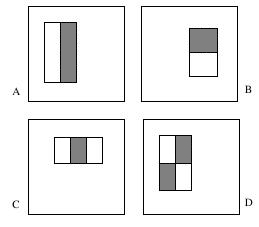
\includegraphics[width=0.5\columnwidth]{ch5/figures/haarfeatures.jpg}
\caption{The four examples of Haar features. \cite{Viola2001}}
\label{fig:haarfeatures}
 \end{center}
\end{figure} 
The sum of the pixels which lie within the white rectangles are subtracted from the sum of pixels in the grey rectangles. These four Haar features are primitives of all Haar features. All Haar features vary with positions, size of rectangle, and the types. The position determines where the Haar feature is in an image. The size of rectangle determines how large the Haar feature is. It also can be considered as the scale of the Haar feature, because with a larger size of rectangles, the Haar feature detects more global variation, whilst with a smaller size of rectangles, the Haar features detects more local precise variation. Among these four examples, there are three primitives of Haar features. For (A), the primitive represents features which detect the horizontal variation of pixels in images. For (B), the primitive represents features which detect the vertical variation of pixels in images. (C) can be considered as an alternative of (A), which also detects the horizontal changes. For (D), the primitive is more complicated than others. There are four rectangles in the primitive, and they are in a skew-symmetric structure. The primitive represents features which detect the diagonal variation of pixels in images. Therefore, Haar features contain three kinds of variations: horizontal variation, vertical variation and skew-symmetric variation.

Haar features are similar to Gabor wavelet features. They both have the position variable. The size of rectangle in Haar features is equivalent to spatial frequency $\nu$ in Gabor wavelet features, which decides the size of Gabor wavelet kernel. The primitives are equivalent to the orientations in the Gabor wavelet features. As there are three primitives, there are three orientations in Haar feature: horizontal (0$^\circ$), vertical (90$^\circ$) and skew-symmetric (45$^\circ$). However, Gabor wavelet features can contain any orientation. To detect the salient change of image in different orientations, Gabor wavelet features are more appropriate than Haar features. In face verification, facial texture is complicated and the salient change could be in different orientations. Gabor wavelet features will provide more precise representation than Haar features do on face verification. In \cite{Wu2004glasses}, both Gabor wavelet features and Haar features are used on glass detection. The results show that the detection algorithm using Gabor wavelet features have better performance than the detection algorithm using Haar features. Therefore, Gabor wavelet features are used to represent faces in this thesis.

In \cite{Shen2006,Yang2004fg}, two similar algorithms of Gabor wavelet features and AdaBoost algorithm are also presented. In these two algorithms, face recognition is not based on classifying subjects, but on classifying \textit{intra-personal difference} and \textit{extra-personal difference} \cite{Moghaddam1997} with difference images between two face images. However, human face image appearance has potentially very large intra-personal difference due to facial expression, occlusion (\textit{e.g.} glasses), lighting, pose, and other issues. On the other hand, the extra-personal difference may be small due to the similarity of individual appearance. \mbox{Figure} \ref{fig:intravsextra} illustrates examples of appearance difference of different subjects. 
\begin{figure}[ht]
 \begin{center}
  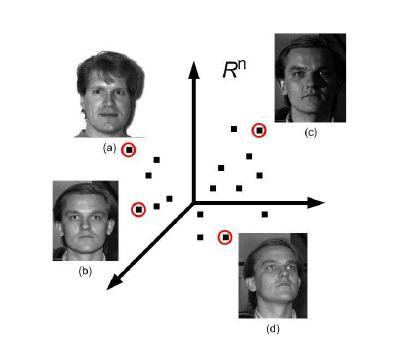
\includegraphics[scale=0.77]{ch5/figures/intravsextra}
  \caption{The Intra-personal difference versus the Extra-personal difference. \cite{Lu2006}}
  \label{fig:intravsextra}
 \end{center}
\end{figure} 
In \mbox{Figure} \ref{fig:intravsextra}, (a) and (b) are images from different people, but their appearance difference in the input space is smaller than images of the same person but with different poses and lighting changes as shown in (c) and (d). Adini \textit{et al.} \cite{Adini1997} demonstrate that the differences between images of the same face due to lighting, viewpoint, and facial expression changes could be larger than those between different face images. Therefore, the intra-personal and extra-personal recognition mechanism may not be appropriate for face verification.

 
\section{Feature pre-selection schemes}
\label{sec:preselection}
As mentioned in \mbox{Section} \ref{sec:gaborwaveletfeature}, a Gabor wavelet feature $j$ is configured by three key parameters, which are the position $z=(x,y)$, the orientation $\mu$, and the spatial frequency $\nu$ (also called scale), so that the number of possible Gabor wavelet features is determined by the number of positions, orientations, and scales. It is common to use the parameters as $\nu\in\{-1,\ldots,3\}$, and $\mu\in\{0,\ldots,7\}$, and the number of position is due to the size of images processed by the Gabor wavelet transform. If all features are used in feature selection, the process will take a very long time to select significant features as face representatives. Three schemes are developed to define the number of positions.
\begin{itemize}
 \item \textbf{Full size} There is no reduction on the number of total features. The number of positions is equal to the original number of pixels;
 \item \textbf{Interlace} The features are sampled column by column and row by row. The number of positions is roughly one quarter of the total number of pixels;
 \item \textbf{Scaling} The response images are scaled down according to the spatial frequency, and the number of positions is reduced.
\end{itemize}

In \textbf{Full size}, the number of positions is the same as the number of pixels in the image, \textit{e.g.}, if there is an image with 64 pixels in the width and 64 pixels in the height, the number of features is $64\times 64 \times 5 \times 8 = 163,840$. If the full size scheme is adapted, unless the size of image is comparatively small, the number of features will be very large. Large numbers of features introduces difficulties to the algorithm, \textit{e.g.}, time-consuming and complexity of design. Hence, it is better to reduce the number of features if possible. The other two schemes are grounded on this concern.

The \textbf{Interlace} scheme is similar to the Interlace technique \cite{Ballard1939} for improving the picture quality of a video signal in the Television industry. After the Gabor wavelet transform on a single image, there are $40$ response images left with the same size as the original image. The scheme is to remove even rows and columns such that only odd rows and columns remain. This makes the number of pixels remaining in the response images roughly one quarter of that in the original image. 

The \textbf{Scaling} scheme is used to reduce the number of features by scaling down these response images with higher spatial frequencies $\nu$. There is a phenomenon that in higher frequency response images, the response images appear blurred. In \mbox{Figure} \ref{fig:lowandhighscalesface} is a $55\times51$ \mbox{XM2VTS} face image. Images in \mbox{Figures} \ref{fig:lowandhighscales-1}, \ref{fig:lowandhighscales0}, \ref{fig:lowandhighscales1}, \ref{fig:lowandhighscales2} and \ref{fig:lowandhighscales3} are the magnitude of response images at frequency $\nu=\{-1,0,1,2,3\}$, respectively, and the orientation is $\frac{\pi}{4}$, \textit{i.e.}, $\mu=2$. As the spatial frequency increases, the response images become more blurred. This indicates that in higher frequency response images, the neighour features are highly correlated. In \mbox{Figures} \ref{fig:lowandhighscales2} and \ref{fig:lowandhighscales3}, human vision perception is unable to distinguish the facial characteristics.
\begin{figure}[ht]
\begin{center}
   \subfigure[]{\label{fig:lowandhighscalesface}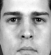
\includegraphics{ch4/figures/xm2vtsone.jpg}}
   \subfigure[]{\label{fig:lowandhighscales-1}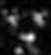
\includegraphics{ch4/figures/response_-1.jpg}}
   \subfigure[]{\label{fig:lowandhighscales0}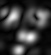
\includegraphics{ch4/figures/response_0.jpg}}
   \subfigure[]{\label{fig:lowandhighscales1}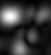
\includegraphics{ch4/figures/response_1.jpg}}
   \subfigure[]{\label{fig:lowandhighscales2}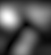
\includegraphics{ch4/figures/response_2.jpg}}
   \subfigure[]{\label{fig:lowandhighscales3}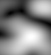
\includegraphics{ch4/figures/response_3.jpg}}
 \caption{The response images from low spatial frequency to higher frequency.}
\label{fig:lowandhighscales}
\end{center}
\end{figure}
In addition, in 2-D discrete convolution, convolving images with high frequency Gabor wavelets is equivalent to scaling down images and convolving with lower frequency Gabor wavelet as shown in \mbox{Figure} \ref{fig:scalingscheme}.
\begin{figure}[t]
 \begin{center}
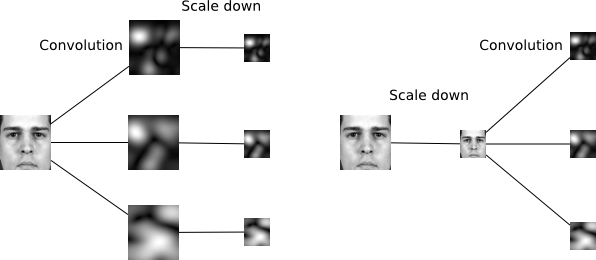
\includegraphics[width=\columnwidth]{ch4/figures/scalingscheme.png}
  \caption{The two processes are equivalent in terms of results.}
  \label{fig:scalingscheme}
 \end{center}
\end{figure} 
In the left of \mbox{Figure} \ref{fig:scalingscheme}, the original face image is firstly convolved by three Gabor wavelets with $\nu = \{1,2,3\}$ to obtain three magnitude responses, then these responses are reduced into the $\frac{1}{4}$ of the original size. On the right of \mbox{Figure} \ref{fig:scalingscheme}, the original face image is firstly reduced to $\frac{1}{4}$ of the original size, then convolved by three Gabor wavelets with $\nu=\{-1,0,1\}$. These magnitude responses are the same as those reduced magnitude responses on the left. The results from \mbox{Figure} \ref{fig:scalingscheme} are magnified in \mbox{Figure} \ref{fig:conv2scaledown}. 
\begin{figure}[ht]
\begin{center}
   \subfigure[]{\label{fig:responsehalf1}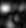
\includegraphics[scale=2]{ch4/figures/response_1_half.jpg}}
   \subfigure[]{\label{fig:responsehalf2}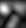
\includegraphics[scale=2]{ch4/figures/response_2_half.jpg}}
   \subfigure[]{\label{fig:responsehalf3}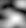
\includegraphics[scale=2]{ch4/figures/response_3_half.jpg}}\\
   \subfigure[]{\label{fig:halfresponse-1}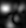
\includegraphics[scale=2]{ch4/figures/eteser_-1_3.jpg}}
   \subfigure[]{\label{fig:halfresponse0}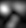
\includegraphics[scale=2]{ch4/figures/eteser_0_3.jpg}}
   \subfigure[]{\label{fig:halfresponse1}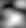
\includegraphics[scale=2]{ch4/figures/eteser_1_3.jpg}}
 \caption{Comparison between response images after convolving with high frequency Gabor wavelet and after convolving with low frequency Gabor wavelet.}
\label{fig:conv2scaledown}
\end{center}
\end{figure}
Images in \mbox{Figures} \ref{fig:responsehalf1}, \ref{fig:responsehalf2} and \ref{fig:responsehalf3} are the results from the left part, while images in \mbox{Figure} \ref{fig:halfresponse-1}, \ref{fig:halfresponse0} and \ref{fig:halfresponse1} are the results from the right part. The top row and the bottom row in \mbox{Figure} \ref{fig:conv2scaledown} show that the responses are identical. The processing in which convolution is first done and then scale down, is equivalent to the processing in which scale down is first and then convolution. \mbox{Figure} \ref{fig:conv2scaledown} also indicates that higher frequency response images can be scaled down into smaller sizes without significant information loss 

Therefore, in the \mbox{Scaling} scheme, the number of features is reduced by scaling down the response images with higher frequencies. For an image with the size $W\times H$, the response image with the lowest frequency is kept to size of $W\times H$. For the second lowest frequency, the size of response images is $\frac{W\times H}{4}$; for the third lowest frequency, the size of response image is $\frac{W\times H}{16}$, and so on. The corresponding number of features are  $W\times H\times 8$, $\frac{W\times H}{2^2}\times 8$, $\frac{W\times H}{2^4}\times 8$ and so on. If the width $W=64$ and the height $H=64$ with five frequencies $\nu=\{-1,\ldots,3\}$ and eight orientations, the total number of features is
\begin{displaymath}
 (W\times H+ \frac{W\times H}{2^2} + \frac{W\times H}{2^4} + \frac{W\times H}{2^6}+ \frac{W\times H}{2^8})\times 8= 43648
\end{displaymath}
With \textbf{Full size}, the total number of features is $163,840$. In the \textbf{Scaling} scheme, the size deduction ratio is $43648/163840\approx 0.27$.

\section{Feature Selection}
\label{sec:featureselection}
After applying the pre-selection scheme to reduce the feature space, the AdaBoost algorithm is applied for feature selection. This section presents the algorithm firstly, and then an elementary part of AdaBoost - FLD weak learner is introduced. 

Feature selection is a technique, commonly used in machine learning and pattern recognition for reducing feature space. It selects a subset of relevant features from a large number of features to construct robust learning models. By removing irrelevant and redundant features from the training data, feature selection helps in improving the performance of learning models. Feature selection also helps to distinguish features which are important for learning. From a theoretical perspective, feature selection for classification or recognition is to obtain an optimal subset from all features against the exhaustive search of all possible subsets.

\subsection{AdaBoost algorithm for Feature Selection}
A variant of AdaBoost is adapted for selecting most important features for face verification. The feature selection algorithm is with respect to individual clients. If the face verification system is required being able to verify all clients, the algorithm will be applied to select the most significant features for each client, such that a small number of features corresponding to each client are collected and constructed into a classifier to verify that client. A feature group is unique for a client. The algorithm for feature selection is listed in \mbox{Table} \ref{tab:adaboostfs}. 
\begin{table}[ht]
\caption{The variant algorithm of AdaBoost for feature selection}
\begin{tabular}{p{\columnwidth}}\\
\hline
\begin{algorithmic}[1]
\STATE Given example $(x_{1},y_{1}),\ldots,(x_{n},y_{n})$, where $x_{i}$ is the data of the $i$th example, which are contributed by $k$ features $\{j_{1},\ldots,j_{k}\}$, and $y_{i} \in Y=\{0,1\}$ for impostor and client, respectively.
\STATE Initialise the weights $\omega_{1,i}=\frac{1}{2m},\frac{1}{2l}$ for $y_{i}=0,1$ respectively, where $m$ and $l$ are the number of impostors and clients, respectively.
\FOR{$t=1,\ldots,T$}
	\STATE Normalise the weights, $\omega_{t,i}\leftarrow\frac{\omega_{t,i}}{\sum_{i=1}^{n}\omega_{t,i}}$ so that $\omega_{t}$ form a probability distribution.
	\FORALL{$\{j_{1},\ldots,j_{k}\}$}
		\STATE Train a weak learner $h_{j}$ which is restricted to use a single feature $j$. 
		\STATE The error is calculated as $\varepsilon_{j}=\sum_{i=1}^{n}\omega_{t,i}|h_{j}(x_{i})-y_{i}|^{2}$ with respect to $\omega_{t,i}$
	\ENDFOR
	\STATE Choose the optimal weak learner $h_{t}$ with the lowest error $\varepsilon_{t}$ from all $h_{j}$.
	\STATE Select the corresponding feature $j_{t}$ from the weak learner $h_{t}$ as a significant feature.
	\STATE Remove the feature $j_{t}$ from the feature set $\{j_{1},\ldots,j_{k}\}$.
	\STATE Update the weights $\omega_{t+1,i}=\omega_{t,i}\beta_{t}^{1-e_{i}}$, where $e_{i}=0$ if example $x_{i}$ is classified correctly and $e_{i}=1$ otherwise, and $\beta_{t}=\frac{\varepsilon_{t}}{1-\varepsilon_{t}}$.	
\ENDFOR
\end{algorithmic}\\
\hline
\end{tabular}
\label{tab:adaboostfs}
\end{table} 
In the learning algorithm, the learning process contains $n$ training examples in the training set. Each example $(x_{i},y_{i})$ is defined such that $x_{i}$ is the data and $y_{i}$ is the label. The data of each example contains $k$ features $\{j_{1},\ldots,j_{k}\}$ which construct a vector with $k$ elements. The label $y_{i}$, also called class of the example, is $0$ or $1$ for impostor or client respectively. 

The example is associated with a weight $\omega$ to indicate how difficult the example for a weak learner is recognised. The allocation of weights on each example is called initialisation. Different from the initialisation in \mbox{Table} \ref{tab:adaboost} of \mbox{Chapter} \ref{ch:gaboradaboost}, in this algorithm, client (positive examples) and impostor (negative examples) are given different weights with respect to the number of corresponding examples in the training set. This is due to the fact that the number of client face images may not be equal to the number of impostor face images in the training set. The weight of an example also indicates prior probability which is referred to prior knowledge of the example in the whole population of examples. When positive and negative examples are well balanced, \textit{i.e.}, the numbers are equal, each example will share the same prior probability $\frac{1}{n}$ if there are $n$ examples. When positive and negative examples are not balanced, the prior probability for a particular class is evaluated by the number of examples in the class dividing the total number of examples. It is assumed that there are $l$ positive examples and $m$ negative examples in the training set, \textit{i.e.}, the whole population $l+m=n$, and both accumulative prior probabilities of positive and negative examples are equal to $0.5$. In the perspective of the vector space, the subspace spanned by positive examples takes half capacity of the vector space, and the subspace spanned by negative examples takes the other half. Within positive examples, the prior probability of each example should be the same. That is because the examples belonging to the same class are of equal importance and no example in the same class will be more important than others at the beginning of AdaBoost learning. Hence, if an example is positive, the weight is $\frac{1}{2l}$, otherwise the weight is $\frac{1}{2m}$ at the initialisation.

After initialising the weights, AdaBoost training is going to the stage of iteration running. The number of iterations in the training is determined by the number of expected selected features. If $T$ features are selected from the whole set of features, the number of iterations will be set to $T$. At the beginning of each iteration, the weights need to be normalised so that all weights form a probability distribution, \textit{i.e.}, the weights are divided by the sum of all weights.

AdaBoost performs an exhaustive search on all features to find the optimal feature. For each feature $j$, the algorithm trains a weak learner $h_{j}$ based on the training examples associated with weights. The weak learner $h_{j}$ is restricted to use one single feature $j$ rather than all features $\{j_{1},\ldots,j_{k}\}$, such that the data of each example is represented by only one numeral in the weak learner. This weak learner is called a single feature based weak learner. After the weak learner $h_{j}$ is trained, the error is calculated with respect to the weights. From \mbox{Table} \ref{tab:adaboostfs}, it can be seen that the error $\varepsilon$ is the sum of the weights whose corresponding examples are misclassified. It is obviously that the range of the error is $0\le \varepsilon \le 1.0$.

After the training is done on all single feature based weak learners, the minimum error $\varepsilon_{t}$ among weak learners is obtained by sorting algorithm. The corresponding weak learner $h$ and feature $j$ are retained. The feature $j$ is labelled as $j_{t}$, which is the selected feature from the iteration $t$. The weak learner $h_{t}$ is the weak learner generated from the same iteration. Also, it is necessary to remove the feature $j_{t}$ from the whole feature set $\{j_{1},\ldots,j_{k}\}$, so that the feature is excluded in the next iteration.

At the end of each iteration, the weights need to be updated according to the performance of the weak learner $h_{t}$.  The weights are updated in order to emphasise those examples which are misclassified by the weak learner $h_{t}$.  If an example is classified correctly by $h_{t}$, the weight $\omega_{t+1,i}$ will be decreased. If an example is misclassified, the weight will be keep the same.


\subsection{Weak Learner: Fisher Linear Discriminant}
\label{sec:faceveri:fld}
The choice of weak learner is crucial for the process of AdaBoost training. Some considerations of weak learners are firstly given, then the FLD (Fisher's Linear Discriminant) weak learner is presented.

\subsubsection{Weak Learner}
A weak learner using a single feature is very important for the AdaBoost feature selection. There are many possible choices for weak learners, such as Artificial Neural Network (ANN), Naive Bayes, Fisher's Linear Discriminant, Support Vector Machine (SVM) and so on. The choice of weak learner is based on two factors:
\begin{itemize}
 \item The computational cost of the weak learner training on a given training set should be low.
 \item The classification accuracy of the weak learner is slightly better than random guess.
\end{itemize}
Firstly, the training time for weak learner should be fast enough, otherwise the overall training of AdaBoost will take an extremely long time. For example, training a weak learner requires $1$ second on a certain computer, and there are $40,000$ features in the training set, so each iteration will take roughly $11$ hours. If the aim is to select $20$ features, the total computational time will be about $9$ days. Hence, it is important to choose a fast weak learner. Secondly, a learner is defined as ``weak'' so it's classification ability is not expected to be strong. The classification accuracy of a weak learner should normally be better than random guessing, which is $0.5$. Hence, an ideal weak learner should be simple and fast. Among those base classifiers mentioned above, a Fisher Linear Discriminant (FLD) weak learner is an appropriate solution in selecting Gabor wavelet features \cite{Ichikawa2006,Kong2006,Asami2005}. The FLD weak learner is fast because it is a linear classifier. Non-linearity requires complex structures like SVM and ANN to produce higher accuracy, but is penalised by more computational cost. The FLD weak learner does not make the assumption on the distribution of each class, such as Naive Bayes does.

\subsubsection{Fisher Linear Discriminant}
Fisher's Linear Discriminant (FLD) comprises methods used in statistics and machine learning to find a linear boundary which best separates two or more classes of objects. FLD was first proposed by R.A. Fisher in 1936 \cite{Fisher1936}. He defined the separation between two class examples to be the ratio of \textit{the variance between the classes} to \textit{the variance within the classes}. For a better classification performance, the ratio should be as small as possible. By maximising the variance between classes and minimising the variance within classes, the classifier can reach the optimal performance. When the ratio is at its minimum, the optimal classifier is found.

The input data for weak learners is one-dimensional examples $x_{1},\ldots, x_{n}$, and $l$ is the number of positive examples, and $m$ is the number of negative examples. Each example is labelled with $y=1$ or $y=0$ as positive or negative respectively. The purpose is to find a good predictor for the class $y$ of any example. The predictor is defined as
\begin{equation}
 y= \textbf{\textrm{w}}x + b
\end{equation}
$\textbf{w}$ is the weight coefficient of the predictor, and $b$ is the bias of the predictor. The problem is how to find $\textbf{w}$ and $b$. The mean of positive examples and negative examples are
\begin{equation}
 \mu_{y=1}=\frac{1}{l}\sum_{y_{i}=1}x_{i}
\end{equation}
\begin{equation}
 \mu_{y=0}=\frac{1}{m}\sum_{y_{i}=0}x_{i}
\end{equation}
so that the variance between classes is $S_{b}=\mu_{y=1}-\mu_{y=0}$, and the variance within the positive class is
\begin{equation}
 S_{w_{y=1}}=\sum_{y_{i}=1} (x_{i}-\mu_{y=1})^2
\end{equation}
and the variance within the negative class is 
\begin{equation}
 S_{w_{y=0}}=\sum_{y_{i}=0} (x_{i}-\mu_{y=0})^2
\end{equation}
The overall variance within classes is $S_{w}=S_{w_{y=1}}+S_{w_{y=0}}$. The solution for the coefficient $\textbf{w}$ optimising the ratio is 
\begin{equation}
 \textbf{w}= S_{w}^{-1}(\mu_{y=1}-\mu_{y=0})
\end{equation}
The means of projected points are 
\begin{equation}
 \widehat{\mu}_{y=1}=\textbf{w}\cdot\mu_{y=1}
\end{equation}
\begin{equation}
 \widehat{\mu}_{y=0}=\textbf{w}\cdot\mu_{y=0}
\end{equation}
The bias $b$ is calculated as
\begin{equation}
 b=-\frac{\widehat{\mu}_{y=1}+\widehat{\mu}_{y=0}}{2}
\end{equation}
Given a set of examples $x_{1},\ldots, x_{n}$ with corresponding label $y=0,1$, the training of the FLD weak learner is to find  \textbf{w} and $b$ to form a predictor. From the training example, it is easy to compute the means and variances.

\subsection{Reduction of Computational Time}
\label{sec:faceveri:time}
In AdaBoost, the error of the final strong classifier is bounded by \mbox{Equation} \ref{eq:trainingerror} in \mbox{Chapter} \ref{ch:gaboradaboost}. Thus, there is one hypothesis for AdaBoost. 
\begin{quote}
\textit{If weak learners that are slightly better than random guessing can be consistently found, then the error of the final strong classifier drops exponentially fast.} \cite{Freund1995}
\end{quote}
If a weak learner is equivalent to random guessing, its classification error will be $0.5$. If a weak learner has its error rate more than $0.5$, this indicates that given a number of labelled examples, more than half the examples are misclassified. Therefore $0.5$ is the limit bounding the error of a weak learner. To have high accuracy in the final classifier, the error of the weak learner should be less than $0.5$. Because in the original AdaBoost (in \mbox{Table} \ref{tab:adaboost}), the weak learner generated from iterations are combined into an ensemble. Any weak learner with low discrimination power will distort the overall performance of the ensemble. Only a weak learner with performance better than random guessing is allowed to be combined into the final classifier. Although, for each weak learner, the error is expected to be as small as possible, with a simple structure and fast running speed, the weak learners can not be guaranteed to achieve very high classification accuracy.

In AdaBoost based feature selection, low recognition accuracy in a weak learner also indicates that the corresponding Gabor wavelet feature is irrelevant or redundant for face verification.  When a weak learner has the error equal or greater than $0.5$, AdaBoost training on the weak learner will stop, because the performance of the classifier can not be boosted. 

For example, in the experiment which will be described in \mbox{Section} \ref{sec:faceveri:result1}, there are $29,120$ features trained in the first iteration. The error distribution of the corresponding $29,120$ weak learners are illustrated in \mbox{Figure} \ref{fig:disterrors}, in which the horizontal axis shows the error and the vertical axis displays the number of weak learners. It can be seen clearly from  \mbox{Figure} \ref{fig:disterrors}, the distribution of the errors from all weak learners looks like a normal distribution with the mean error at $0.35$. Most errors of the weak learners are in the range $0.2$ to $0.5$. There are some weak learners whose errors are equal or greater than $0.5$, \textit{i.e.}, error of random guessing.
 \begin{figure}[ht]
 \begin{center}
   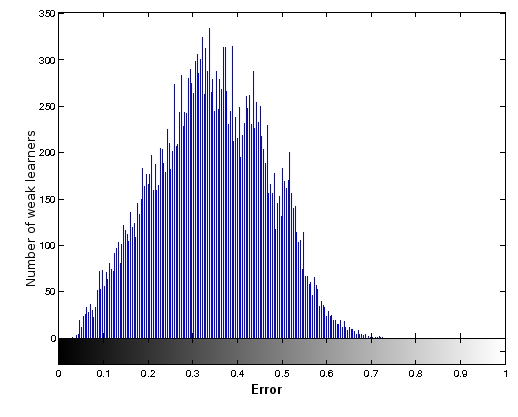
\includegraphics[width=\columnwidth]{ch4/figures/disterrors.png}
  \caption{The distribution of the error of all weak learners}
 \label{fig:disterrors}
 \end{center}
 \end{figure} 
All weak learners having performance worse than random guessing will stop in training at the next iteration. The corresponding feature will be discarded at the next iteration to build a weak learner.

The AdaBoost algorithm for feature selection is modified in \mbox{Table} \ref{tab:retimeadaboostfs}. 
\begin{table}[ht]
\caption{The improved algorithm of AdaBoost for feature selection}
\begin{tabular}{p{\columnwidth}}
\hline
\begin{algorithmic}[1]
\STATE Given example $(x_{1},y_{1}),\ldots,(x_{n},y_{n})$, where $x_{i}$ is the data of the $i$th example, which are contributed by a set $J$ including $k$ features $\{j_{1},\ldots,j_{k}\}$, and $y_{i} \in Y=\{0,1\}$ for impostor and client respectively..
\STATE Initialise the weights $\omega_{1,i}=\frac{1}{2m},\frac{1}{2l}$ for $y_{i}=0,1$ respectively, where $m$ and $l$ are the number of impostors and clients respectively.
\FOR{$t=1,\ldots,T$}
	\STATE Normalise the weights, $\omega_{t,i}\leftarrow\frac{\omega_{t,i}}{\sum_{i=1}^{n}\omega_{t,i}}$ so that $\omega_{t}$ form a probability distribution.
	\FORALL{$j$ in the set $J$}
		\STATE Train a weak learner $h_{j}$ which is restricted to use a single feature $j$. 
		\STATE The error is calculated as $\varepsilon_{j}=\sum_{i=1}^{n}\omega_{t,i}|h_{j}(x_{i})-y_{i}|^{2}$ with respect to $\omega_{t,i}$
		\IF{$\varepsilon \ge 0.5$}
			\STATE Remove the feature $j$ from the set $J$.
		\ENDIF
	\ENDFOR
	\STATE Choose the optimal weak learner $h_{t}$ with the lowest error $\varepsilon_{t}$ from all $h_{j}$.
	\STATE Select the corresponding feature $j_{t}$ of the weak learner $h_{t}$ as a significant feature.
	\STATE Select the feature $j_{t}$ out of the set $J$.
	\STATE Update the weights $\omega_{t+1,i}=\omega_{t,i}\beta_{t}^{1-e_{i}}$, where $e_{i}=0$ if example $x_{i}$ is classified correctly and $e_{i}=1$ otherwise, and $\beta_{t}=\frac{\varepsilon_{t}}{1-\varepsilon_{t}}$.	
\ENDFOR
\end{algorithmic}\\
\hline
\end{tabular}
\label{tab:retimeadaboostfs}
\end{table} 
In this improved algorithm, a feature set $J$ is defined, which contains all features $\{j_{1},\ldots,j_{k}\}$ at the beginning of AdaBoost training. In each iteration, only one significant feature is selected, and some features are removed from the set $J$.  In each iteration, the exhaustive search is on the set $J$ rather than on all features $\{j_{1},\ldots,j_{k}\}$.


\section{Experiments}
\label{sec:experiments}
The eXtended Multi Modal Verification for Teleservices and Security (XM2VTS) face database is used in the experiments. A small group with $200$ face images and a large group with $800$ face images of experiments are performed on feature selection. Based on the selected features from the large group of experiments, an SVM classifier is trained for face verification.

\subsection{XM2VTS Face Database}
\label{sec:faceveri:xm2vts}
The developed feature selection algorithm was tested in XM2VTS \cite{Messer1999}. The XM2VTS database is a multi-modal face database which is captured onto high quality digital video. The XM2VTS includes colour images, sound files, video sequences and 3D Models. The XM2VTS contains four sessions of 295 subjects recorded over a period of four months at approximately one month intervals.
% Each session includes a speaking head shot and a rotating head shot as shown in \mbox{Figure} \ref{fig:XM2VTS}. 
% \begin{figure}[ht]
%  \begin{center}
%   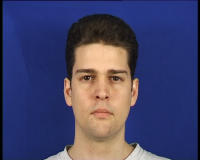
\includegraphics[width=\textwidth/4]{ch4/figures/charles_c1.jpg}
%   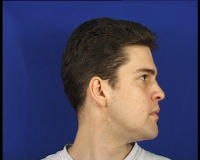
\includegraphics[width=\textwidth/4]{ch4/figures/charles_l1.jpg}
%   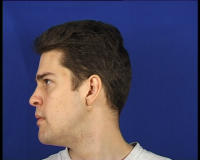
\includegraphics[width=\textwidth/4]{ch4/figures/charles_r1.jpg}\\
%   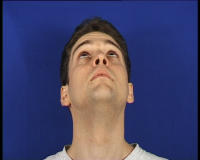
\includegraphics[width=\textwidth/4]{ch4/figures/charles_u1.jpg}
%   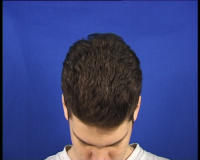
\includegraphics[width=\textwidth/4]{ch4/figures/charles_d1.jpg}
%   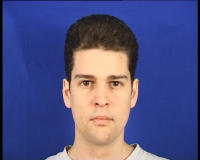
\includegraphics[width=\textwidth/4]{ch4/figures/charles_c2.jpg}
%   \caption{The speaking head shot and rotating head shots from XM2VTS}
%   \label{fig:XM2VTS}
%  \end{center}
% \end{figure} 
% On each visit of every subject, two shots were made. The first shot consisted of speech while the second shot consisted of rotating head action. A Sony VX1000E digital cam-corder and a DHR1000UX digital VCR were used to capture the database. This captures video at a colour sampling resolution of 4:2:0 and audio at frequency 32kHz and sampling rate of 16 bit. At the third shot a high-precision 3D model of the subjects head was built using an active stereo.

In XM2VTS, there are $295$ subjects with $200$ clients and $95$ impostors. Since only the frontal face images are concerned, for each subject 8 up-right and frontal view images have been used. The database was divided into three sets: training set, evaluation set, and testing set. The training set is used to build face models. The evaluation set is for selection of a threshold that determines if a person is accepted or rejected. The testing set is to test the performance of the algorithm. In face verification, a person is accepted if he is a legal client; a person is rejected if he is an impostor. The features are extracted and selected in face images from the training set which includes 200 clients with the first 4 images of each client. In the evaluation set, two face images across $200$ clients and $8$ images across $20$ impostors are collected. In the testing set, two images across $200$ clients and $8$ images from 75 new impostors are used. The images are selected to take account of moderating differences in illumination, expressions and facial details. 

Each subject has $8$ frontal images. The images are stored in colour PPM format \cite{ wiki:ppm} and at resolution $720\times576$. To perform feature selection and face verification, the images need to be adjusted and segmented, because these large images not only contain inner face area but also the background, the hair, the necks, and so on. The redundant areas such as background, hair, etc, are irrelevant for the face verification application. The segmentation to obtain only the inner face area is performed. Due to the appearance based approach adopted, for segmenting a face image, some reference points are needed to correspond with all face images. In this thesis, the two pupils on the face are the reference points to segment inner face images. The following steps are taken in the processing.
\begin{enumerate}
 \item If two pupils on a face image are not on the same horizontal line, the image will be rotated to make the two pupils horizontal.
 \item The distance between the pupils is measured. The face image is scaled so that the distance between the pupils is $26$ pixels.
 \item The image is segmented by using a window $55$ pixels high and $51$ pixels wide. The left pupil is matched with position $(13,19)$, and the right pupil is matched with position $(39,19)$ in the window.
 \item The segmented image is converted into gray-scale.
\end{enumerate}
Therefore, all images are properly rotated, scaled, segmented and converted to fit a grid size of $55\times51$ as illustrated in \mbox{Fig} \ref{fig:XM2VTSface}.
\begin{figure}[ht]
\begin{center}
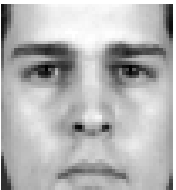
\includegraphics[scale=0.12]{ch4/figures/XM2VTS_1.png}
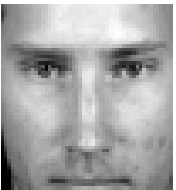
\includegraphics[scale=0.12]{ch4/figures/XM2VTS_2.png}
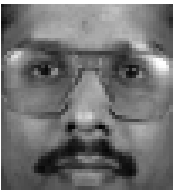
\includegraphics[scale=0.12]{ch4/figures/XM2VTS_3.png}
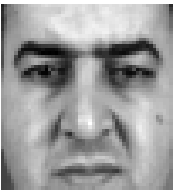
\includegraphics[scale=0.12]{ch4/figures/XM2VTS_4.png}
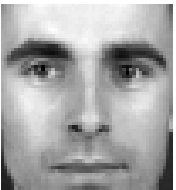
\includegraphics[scale=0.12]{ch4/figures/XM2VTS_5.png}
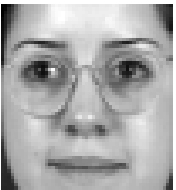
\includegraphics[scale=0.12]{ch4/figures/XM2VTS_6.png}
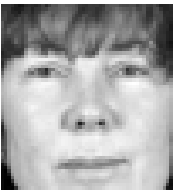
\includegraphics[scale=0.12]{ch4/figures/XM2VTS_7.png}
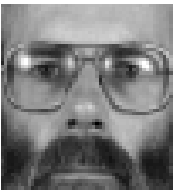
\includegraphics[scale=0.12]{ch4/figures/XM2VTS_8.png}\\
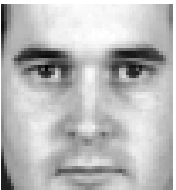
\includegraphics[scale=0.12]{ch4/figures/XM2VTS_9.png}
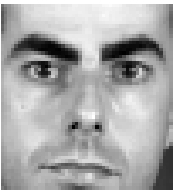
\includegraphics[scale=0.12]{ch4/figures/XM2VTS_10.png}
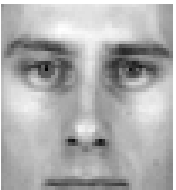
\includegraphics[scale=0.12]{ch4/figures/XM2VTS_11.png}
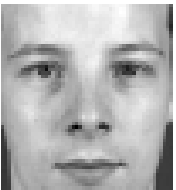
\includegraphics[scale=0.12]{ch4/figures/XM2VTS_12.png}
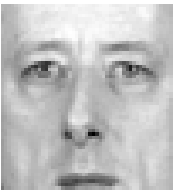
\includegraphics[scale=0.12]{ch4/figures/XM2VTS_13.png}
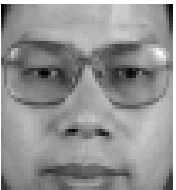
\includegraphics[scale=0.12]{ch4/figures/XM2VTS_14.png}
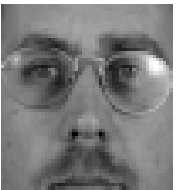
\includegraphics[scale=0.12]{ch4/figures/XM2VTS_15.png}
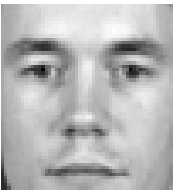
\includegraphics[scale=0.12]{ch4/figures/XM2VTS_16.png}\\
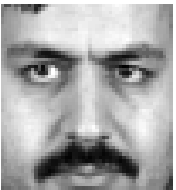
\includegraphics[scale=0.12]{ch4/figures/XM2VTS_17.png}
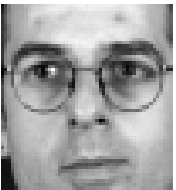
\includegraphics[scale=0.12]{ch4/figures/XM2VTS_18.png}
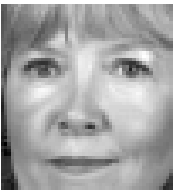
\includegraphics[scale=0.12]{ch4/figures/XM2VTS_19.png}
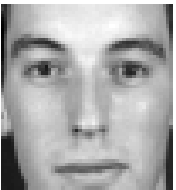
\includegraphics[scale=0.12]{ch4/figures/XM2VTS_20.png}
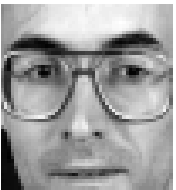
\includegraphics[scale=0.12]{ch4/figures/XM2VTS_21.png}
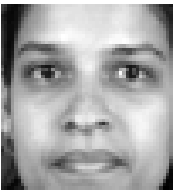
\includegraphics[scale=0.12]{ch4/figures/XM2VTS_22.png}
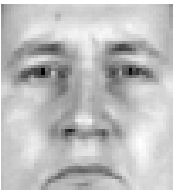
\includegraphics[scale=0.12]{ch4/figures/XM2VTS_23.png}
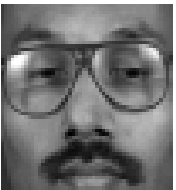
\includegraphics[scale=0.12]{ch4/figures/XM2VTS_24.png}\\
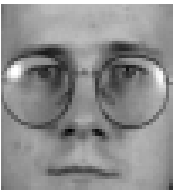
\includegraphics[scale=0.12]{ch4/figures/XM2VTS_25.png}
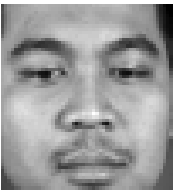
\includegraphics[scale=0.12]{ch4/figures/XM2VTS_26.png}
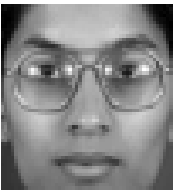
\includegraphics[scale=0.12]{ch4/figures/XM2VTS_27.png}
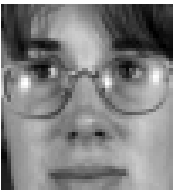
\includegraphics[scale=0.12]{ch4/figures/XM2VTS_28.png}
\includegraphics[scale=0.12]{ch4/figures/XM2VTS_29.png}
\includegraphics[scale=0.12]{ch4/figures/XM2VTS_30.png}
\includegraphics[scale=0.12]{ch4/figures/XM2VTS_31.png}
\includegraphics[scale=0.12]{ch4/figures/XM2VTS_32.png}\\
\includegraphics[scale=0.12]{ch4/figures/XM2VTS_33.png}
\includegraphics[scale=0.12]{ch4/figures/XM2VTS_34.png}
\includegraphics[scale=0.12]{ch4/figures/XM2VTS_35.png}
\includegraphics[scale=0.12]{ch4/figures/XM2VTS_36.png}
\includegraphics[scale=0.12]{ch4/figures/XM2VTS_37.png}
\includegraphics[scale=0.12]{ch4/figures/XM2VTS_38.png}
\includegraphics[scale=0.12]{ch4/figures/XM2VTS_39.png}
\includegraphics[scale=0.12]{ch4/figures/XM2VTS_40.png}\\
\includegraphics[scale=0.12]{ch4/figures/XM2VTS_41.png}
\includegraphics[scale=0.12]{ch4/figures/XM2VTS_42.png}
\includegraphics[scale=0.12]{ch4/figures/XM2VTS_43.png}
\includegraphics[scale=0.12]{ch4/figures/XM2VTS_44.png}
\includegraphics[scale=0.12]{ch4/figures/XM2VTS_45.png}
\includegraphics[scale=0.12]{ch4/figures/XM2VTS_46.png}
\includegraphics[scale=0.12]{ch4/figures/XM2VTS_47.png}
\includegraphics[scale=0.12]{ch4/figures/XM2VTS_48.png}\\
\includegraphics[scale=0.12]{ch4/figures/XM2VTS_49.png}
\includegraphics[scale=0.12]{ch4/figures/XM2VTS_50.png}
\includegraphics[scale=0.12]{ch4/figures/XM2VTS_51.png}
\includegraphics[scale=0.12]{ch4/figures/XM2VTS_52.png}
\includegraphics[scale=0.12]{ch4/figures/XM2VTS_53.png}
\includegraphics[scale=0.12]{ch4/figures/XM2VTS_54.png}
\includegraphics[scale=0.12]{ch4/figures/XM2VTS_55.png}
\includegraphics[scale=0.12]{ch4/figures/XM2VTS_56.png}\\
\includegraphics[scale=0.12]{ch4/figures/XM2VTS_57.png}
\includegraphics[scale=0.12]{ch4/figures/XM2VTS_58.png}
\includegraphics[scale=0.12]{ch4/figures/XM2VTS_59.png}
\includegraphics[scale=0.12]{ch4/figures/XM2VTS_60.png}
\includegraphics[scale=0.12]{ch4/figures/XM2VTS_61.png}
\includegraphics[scale=0.12]{ch4/figures/XM2VTS_62.png}
\includegraphics[scale=0.12]{ch4/figures/XM2VTS_63.png}
\includegraphics[scale=0.12]{ch4/figures/XM2VTS_64.png}\\
\caption{The XM2VTS images after rotation, segmentation and scaling}
\label{fig:XM2VTSface}
\end{center}
\end{figure}

\subsection{Feature Selection Results}
\label{sec:faceveri:result1}
The experiment includes feature extraction and feature selection. The images used are all those in the training set. In the training set, there are $4$ images per client across $200$ clients. $40$ Gabor wavelets are generated according to \mbox{Equation} (\ref{eq:kernel}) with $\nu\in\{0,\ldots,4\}$, and $\mu\in\{0,\ldots,7\}$. Each image is convolved with these $40$ wavelets. The outputs are $40$ magnitude responses for each image. Each point in a magnitude response image corresponds to a feature. The features $O_{\mu,\nu}(z)$ vary with three parameters: orientation $\mu$, scale $\nu$, and position $z$. For each client, there are $8\times5\times55\times51=112,200$ features generated as input for feature selection in each iteration of AdaBoost. The edge of image is discarded due to edge effects caused by convolution. The second method is to apply the \textbf{Interlace} scheme to reduce the number of features. The actual size of each image is reduced to $24\times25$. Consequently the number of features for each image is reduced to $8\times5\times24\times25=24,000$ instead of $112,200$ features.

For each image, there are $24,000$ features generated by Gabor wavelet transform. Two groups of experiments are carried out.
\begin{itemize}
 \item In the first group, a small training set is used. The training set only contains the first 50 subjects of the XM2VTS with $4$ images per subject. For each client, $4$ images are taken as positive examples, and the other $196$ images are taken as negative examples.
 \item In the second group, a large training set is used, which includes all $200$ clients in the XM2VTS database. For each client, $4$ images are taken as positive examples, and the other $796$ images are taken as negative examples.
\end{itemize}
 
This approach gives a large number of training data which are required by the AdaBoost algorithm. However it leaves the ratio between positive and negative examples unbalanced, such as $4/196$ and $4/796$.

\subsubsection{Dealing with more than one minimum errors}
The feature is selected with the lowest error of the corresponding weak learners. However, in some situations (especially with a small training set) there are more than one weak learners sharing the same lowest error. This presents the problem on how to select features and how to update weights. In this thesis, if the situation occurs, in the current iteration, all features which share the same lowest error are selected as the significant features. The weights are updated according to each selected feature associated with a weak learner separately, and the updated weights are the average weight for all features with the same minimum error. To avoid the problem of multiple lowest errors, the solution is to adopt a larger training set.

\subsubsection{Result on the small training set}
For the small training set, the top 20 features are shown in \mbox{Figure} \ref{fig:resultssmall}. 
\begin{figure}[h]
\centering
\subfigure[The 1st client]{\label{fig:20featureson1stsmall}\includegraphics[scale=0.5]{ch4/figures/20featureson1stsmall.png}}
\subfigure[The 4th client]{\label{fig:20featureson4thsmall}\includegraphics[scale=0.5]{ch4/figures/20featureson4thsmall.png}}
\caption{The Gabor wavelet features selected in the first group experiment.}
\label{fig:resultssmall}
\end{figure}
The weak learners associated with these features have the same classification errors, which are equal to zero during AdaBoost feature selection. For the first client, the top 20 features are mostly located on the person's right temple and beside the left eyebrow. \mbox{Figure} \ref{fig:20featureson1stsmall} shows these features on the first client face. The locations of the first 20 features (marked with red crosses) selected for the first client by AdaBoost are shown. These features indicate that the left eyebrow and right-upper temple are significant features for the first client which discriminate that client from others. Most features distributed into two local regions are highly correlated and redundant, as explained in \cite{Penev1996}. In the fourth client, the top $20$ features are located on the person's cheek near the nostril which appears as a deep valley and a nevus on his left face as shown in \mbox{Figure} \ref{fig:20featureson4thsmall}. These are important signs for the fourth client which discriminate that client from others. These features are also highly correlated.

\subsubsection{Result on the large training set}
For the large training set, all $800$ images from the $200$ clients were used. The AdaBoost algorithm selected the top $20$ features from the first client to the 8th client as shown in \mbox{Figure} \ref{fig:resultlarge}.
\begin{figure}[ht]
\begin{center}
\includegraphics[width=\textwidth/9]{ch4/figures/NoC1.png}
\includegraphics[width=\textwidth/9]{ch4/figures/NoC2.png}
\includegraphics[width=\textwidth/9]{ch4/figures/NoC3.png}
\includegraphics[width=\textwidth/9]{ch4/figures/NoC4.png}
\includegraphics[width=\textwidth/9]{ch4/figures/NoC5.png}
\includegraphics[width=\textwidth/9]{ch4/figures/NoC6.png}
\includegraphics[width=\textwidth/9]{ch4/figures/NoC7.png}
\includegraphics[width=\textwidth/9]{ch4/figures/NoC8.png}\\
\includegraphics[width=\textwidth/9]{ch4/figures/Gabor1.png}
\includegraphics[width=\textwidth/9]{ch4/figures/Gabor2.png}
\includegraphics[width=\textwidth/9]{ch4/figures/Gabor3.png}
\includegraphics[width=\textwidth/9]{ch4/figures/Gabor4.png}
\includegraphics[width=\textwidth/9]{ch4/figures/Gabor5.png}
\includegraphics[width=\textwidth/9]{ch4/figures/Gabor6.png}
\includegraphics[width=\textwidth/9]{ch4/figures/Gabor7.png}
\includegraphics[width=\textwidth/9]{ch4/figures/Gabor8.png}\\
\caption{The Gabor wavelet features selected after AdaBoost training in the second group experiment}
\label{fig:resultlarge}
\end{center}
\end{figure}
Some features overlap because they share the same position, but with different orientation or scale. The first feature selected for each client is shown in the bottom row of \mbox{Figure} \ref{fig:resultlarge}. The results shows that the selected features are randomly distributed in the face area rather than concentrated on particular regions of the faces as are the results from the small training set. This indicates that these features are less correlated and less redundant than the features selected in the small training set. Most features are located on eyes, eyebrows, nose, lips, glasses frames or beard. 

Compared to the high correlation among the features in the small training set, the features selected from the large training set can be treated as representatives of local regions. The experiments in the large example size separate the features sparsely, and lead to decorrelation and redundancy reduction. From \mbox{Figure} \ref{fig:resultlarge}, the top $20$ features for different individuals are located in different positions. Although most features correspond to the common key characteristics on a face, \textit{e.g.}, eyes, eyebrows, nostril, lips and so on, the top selected features for each individual are varied. As concluded in \cite{Penev1996}, different subjects can be classified depending on what objects they contain, the faces can be classified depending on the unique characteristics in which an individual is different from others, \textit{e.g.}, the nevus on the left face of the fourth client is a unique characteristics for this person. There are some common features selected in both the large and small training sets as shown in \mbox{Figure} \ref{fig:resultslarge14}. In \mbox{Figure} \ref{fig:1stgaborson1stlarge}, the first selected feature in the large training set is in the eyebrow region, where this is also selected in the small training set. For the fourth client in \mbox{Figure} \ref{fig:1stgaborson4thlarge}, the first selected feature corresponds to the nevus on the left face in the small training set. 
\begin{figure}[ht]
\begin{center}
 \subfigure[The 1st client]{\label{fig:1stgaborson1stlarge}\includegraphics[scale=0.475]{ch4/figures/1stfeatureon1st.png}}
 \subfigure[The 4th client]{\label{fig:1stgaborson4thlarge}\includegraphics[scale=0.475]{ch4/figures/1stfeatureon4th.png}}
 \caption{Common features selected in both the large and small training set }
\label{fig:resultslarge14}
\end{center}
\end{figure}
The selected features for the first client and the fourth client in the small training set are shown in \mbox{Table} \ref{tab:1stclient} and \mbox{Table} \ref{tab:4thclient}, respectively.
\begin{table}[p]
 \caption{The top 20 features selected by the AdaBoost for the first client in XM2VTS.}
\begin{center}
 \centering
  \begin{tabular}{|c|c|c||c|c|c|}\hline
   \small{Scale $\nu$} & \small{Orientation $\mu$} & \small{Position $(x,y)$} & \small{Scale $\nu$} & \small{Orientation $\mu$} & \small{Position $(x,y)$}\\\hline
   1&7&(5,3)&2&4&(49,15)\\\hline
   1&4&(45,13)&2&4&(49,11)\\\hline
   1&4&(47,13)&2&4&(47,15)\\\hline
   1&6&(5,3)&2&4&(45,15)\\\hline
   2&4&(45,11)&0&7&(5,3)\\\hline
   2&4&(45,13)&0&6&(5,3)\\\hline
   2&4&(47,13)&0&6&(3,5)\\\hline
   2&4&(47,11)&1&0&(5,5)\\\hline
   2&4&(49,13)&0&7&(3,3)\\\hline
   1&0&(5,3)&1&6&(39,13)\\\hline
  \end{tabular}
 \label{tab:1stclient}
\end{center}
\end{table}
\begin{table}[p]
 \caption{The top 20 features selected by the AdaBoost for the fourth client in XM2VTS.}
\begin{center}
  \begin{tabular}{|c|c|c||c|c|c|}\hline
   \small{Scale $\nu$} & \small{Orientation $\mu$} & \small{Position $(x,y)$} & \small{Scale $\nu$} & \small{Orientation $\mu$} & \small{Position $(x,y)$}\\\hline
   0&0&(34,35)&1&0&(35,36)\\\hline
   0&0&(35,35)&1&0&(36,36)\\\hline
   0&0&(36,35)&1&6&(46,33)\\\hline
   0&7&(36,36)&1&6&(46,34)\\\hline
   1&0&(34,34)&1&6&(47,34)\\\hline
   1&0&(35,34)&1&7&(45,32)\\\hline
   1&0&(34,35)&1&7&(34,35)\\\hline
   1&0&(35,35)&1&7&(35,35)\\\hline
   1&0&(36,35)&1&7&(36,35)\\\hline
   1&0&(34,36)&1&7&(36,36)\\\hline
  \end{tabular}
 \label{tab:4thclient}
\end{center}
\end{table}
For the first client, most features are distributed into two clusters: one consists of 8 features with the scale and the orientation fitted to 2 and 4 separately.

\subsubsection{Time reduce}
Both algorithms in \mbox{Table} \ref{tab:adaboostfs} and \mbox{Table} \ref{tab:retimeadaboostfs} have been implemented. The algorithm that excludes the big error weak learners displays a significant computational improvement over the original one. The comparison of the two algorithms on time cost is shown in \mbox{Figure} \ref{fig:comparison}. 
\begin{figure}[ht]
\begin{center}
  \includegraphics[width=\textwidth]{ch4/figures/comparison.jpg}
\caption{The comparison of the improved algorithm and the original algorithm on computational time}
\label{fig:comparison}
\end{center}
\end{figure} 
The horizontal coordinate indicates which iteration the AdaBoost training is on, and the vertical coordinate shows the number of features trained in the corresponding iteration. The colour lilac shows the number of features without using the computational time reduction technique, and the colour purple shows the number of features using the technique. In the first iteration, there are $24,000$ Gabor wavelet features ready for AdaBoost training. After the first iteration, $2,177$ weak learners have an error greater than $0.5$, and the corresponding features are excluded from the set $J$, such that there are $21,822$ features remain for the second iteration. In each iteration, some features are removed. In the 20th iteration, only $6,194$ features remain. In the total 20 iterations, computational time is reduced to $54.23\%$ of the original time. If there are more than $20$ iterations in the training, the computation time will be reduced to much less than $54.23\%$ of the original time. Therefore, the approach which excludes some big error weak learners can reduce the computational cost significantly.

\subsection{Classification Results}
\label{sec:faceveri:result2}
With the $20$ Gabor wavelet features selected for each client, a face image is represented by a vector of $20$ features. Verification is performed on the training set and the testing set by using a Support Vector Machine (SVM) \cite{Osuna1997} on each client (subject).

\subsubsection{SVM}
SVMs are a collection of learning approaches used for generalised linear classification. A special property of SVMs is that they minimise the classification error and maximise the geometric margin, so that SVMs are also known as maximum margin classifiers. For two-class classification, it is assumed that there is a hyperplane (also called a \textit{decision boundary}) separating the clusters of two classified data. SVMs project input vectors to a higher dimensional space where a maximal separating hyperplane is created. The separating hyperplane maximises the distance between the two classes. An assumption is made that the larger the margin or distance between two classes, the lower the generalisation error of the classifier will be. SVMs are used to maximise the margin between classes and minimise a quantity proportional to the number of mis-classification errors. The original optimal hyperplane algorithm is a linear classifier. However,  non-linear SVMs can be created by applying the kernel method \cite{Taylor2004} to maximum-margin hyperplanes. The algorithm is allowed to fit the maximum-margin hyperplane in the modified feature space. The classifier is a hyperplane in the high-dimensional feature space, which may be non-linear in the original input space. The kernels can be adopted as a polynomial kernel, a radial based kernel, or a Gaussian radial basis kernel. In this thesis, a Matlab toolbox named OSU Support Vector Machines (SVMs) Toolbox \cite{Ma2001} is used to perform the task of classification.

\subsubsection{Results}
Experiments were carried out on eight clients from the XM2VTS. A non-linear SVM classifier with a polynomial kernel of degree $3$ was constructed from the $800$ training examples, which are the first four images across all clients. The testing set is composed from the other four images across all clients and the eight images across all impostors in XM2VTS. The test results of $8$ clients with $1,560$ testing examples (among them, $4$ positive examples and $1,556$ negative examples from $199$ clients with $4$ images and $95$ impostors with $8$ images per subject) are shown in \mbox{Table} \ref{tab:SVMRe} with the false negative rate $\mathcal{FN}$ and the false positive rate $\mathcal{FP}$.
\begin{table}[ht]
\caption{The classification results from client 1 to client 8 (C1 to C8) with 20 features in XM2VTS.}
 \begin{center}
   \begin{tabular}{|c|c|c|c|c|}
  \hline
    & \multicolumn{2}{c|}{Training Set (\%)} & \multicolumn{2}{c|}{Testing Set (\%)}\\
   \cline{2-5}
  Client & $\mathcal{FN}$ & $\mathcal{FP}$ & $\mathcal{FN}$ & $\mathcal{FP}$ \\
  \hline
  1 & 0.0 & 0.0 & 0.0 & 0.0\\
  2 & 0.0 & 0.0 & 50.0 & 0.0\\
  3 & 0.0 & 0.0 & 50.0 & 0.0\\
  4 & 0.0 & 0.0 & 75.0 & 0.0\\
  5 & 0.0 & 0.0 & 50.0 & 0.0\\
  6 & 0.0 & 0.0 & 50.0 & 0.0\\
  7 & 0.0 & 0.0 & 100.0 & 0.38\\
  8 & 0.0 & 0.0 & 100.0 & 0.0\\
  \hline
 \end{tabular}
 \end{center}
\label{tab:SVMRe}
\end{table} 
By adjusting the bias of each SVM classifier for each client, the false negative rate $\mathcal{FN}$ is set to $0\%$, $25\%$, $50\%$, $75\%$ or $100\%$, and the corresponding classification error (Error rate) and false positive rates are shown in \mbox{Table} \ref{tab:SVMResults}. 
\begin{table}[ht]
\caption{The classification results from client 1 to client 8 (C1 to C8) in XM2VTS with shifting bias}
\begin{center}
\begin{tabular}{|c||c|c|c|c|}
\hline
{False($\%$)}&\multicolumn{4}{c|}{Error rate($\%$)/False Positive rate($\%$)}\\
\cline{2-5}
{Negative}&{C1}&{C2}&{C3}&{C4}\\
\hline
{0}&{4.94/4.95}&{13.72/13.75}&{8.53/8.55}&{2.95/2.96}\\
{25}&{1.73/1.67}&{12.12/12.08}&{11.10/8.29}&{0.26/0.20}\\
{50}&{0.83/0.71}&{8.72/8.61}&{9.58/7.13}&{0.32/0.19}\\
{75}&{0.38/0.19}&{1.41/1.22}&{8.30/6.10}&{0.32/0.13}\\
{100}&{0.26/0.0}&{0.58/0.32}&{2.12/1.35}&{0.26/0.0}\\
\cline{2-5}
\cline{2-5}
&{C5}&{C6}&{C7}&{C8}\\
\cline{2-5}
{0}&{2.31/2.31}&{81.92/82.13}&{53.08/53.21}&{15.64/15.68}\\
{25}&{0.45/0.39}&{14.81/14.78}&{46.47/46.53}&{8.59/8.55}\\
{50}&{0.38/0.26}&{1.86/1.74}&{44.49/44.47}&{0.51/0.39}\\
{75}&{0.38/0.19}&{0.51/0.32}&{6.47/36.38}&{0.38/0.19}\\
{100}&{0.32/0.06}&{0.26/0.0}&{0.64/0.39}&{0.32/0.06}\\
\hline
\end{tabular}
\label{tab:SVMResults}
\end{center}
\end{table}
The optimal boundary for a SVM classifier gives a low error rate but a high false negative rate because the ratio between the positive examples and the negative examples remains unbalanced \footnote{It is also called \textit{selection-bias} or \textit{example-bias}. \mbox{Section} \ref{sec:overfitting} gives the detail.}.  Therefore, the decision surface gets close towards the actual boundary of the negative class, but far away from the place where the positive class resides in the feature space. Moreover, SVMs are only concerned with the trade off between margin and mis-classification error, but not with the false negative rate. This leads to the trained SVM classifiers having strong ability to recognise the negative examples, but relatively weak ability to recognise the positive examples. It also makes the false positive rate much closer to the classification error rate. By adjusting the bias of the SVM classifier, the false  rate can be reduced, while the classification error rate is increased, or {\it vice versa}, {\it e.g.} for client 4, the optimal boundary of the SVM classifier gives the false negative rate equal to $25\%$, and the error rate is $0.26\%$. However, when the bias of the classifier is adjusted, no false negative is detected, and the error rate is increased to $2.95\%$. \mbox{Table} \ref{tab:SVMResults} shows that the classification of clients 1, 4 and 5 has better performance than for other clients. It indicates that the $20$ selected features contribute well enough for some clients to verification, but they are not sufficient to verify some other clients {\it e.g.} clients 6 and 7. In these cases, it may need more features selected by AdaBoost for client representation.

\subsection{Discussion on SVMs in Face Verification}
The ratio between the number of positive and negative examples is unbalanced. Whether in the small or large training set, the number of positive examples is much less than the number of negative examples. Hence, in the feature space, the subspace which all positive examples dominate is much smaller than the subspace which all negative examples dominate. The negative set contains sufficient data which could describe the generality of all negative examples, however the positive set only has $4$ examples, which contains insufficient data to describe itself.

Each example is hypothesised as a point in a two-dimensional feature space as in \mbox{Figure} \ref{fig:hypothesisSVM}. 
\begin{figure}[ht]
\begin{center}
 \includegraphics[width=\columnwidth]{ch4/figures/SVMresult.png}
\caption{The hypothesis on the SVM classification results}
\label{fig:hypothesisSVM}
\end{center}
\end{figure} 
The blue stars and blue circles represent the positive training examples and testing examples, respectively. The red star and red circles represent the negative training and testing examples. The blue solid line denotes the actual boundary for the positive examples, while the blue dash line denotes the predicted boundary for the positive examples. The predicted boundary means that the boundary is predicted by the SVM classifier, rather than the actual boundary of the examples. For the negative examples, the red solid line and dash line indicate the actual boundary and predicted boundary respectively. Most negative training examples and testing examples are concentrated in the right part of \mbox{Figure} \ref{fig:hypothesisSVM}, while positive examples amass in the left part. The actual boundary for the negative is close to the predicted boundary, which indicates the SVM classifier has achieved a good performance on recognising the negative examples. However, the predicted boundary for the positive is far from the actual boundary, which indicates the bad performance on positive examples. The reason is, the positive training examples do not overlap well with the positive testing examples. Some positive examples are recognised as non-positive, because they are out of the predicted boundary. To avoid imbalance on positive and negative, an increase in the number of new positive examples could be useful.

\paragraph{The size of training data}
From the perspective of machine learning, to train ``ability'' on a machine, a data set must be given to the machine to extract information and to learn the relevant decision rules. To build a data set for training (or learning), there is a trade-off between \textbf{representatives} of the training set, \textbf{conciseness} of the training set and \textbf{prior probability} of classes. The representatives of data indicate how much the data covers all the possible variants. The more data in the data set, the higher the representatives are. The conciseness of the data refers to the size of the data set. If the size is big, the conciseness of the data set is poor. As long as the examples are sufficiently representative, the number of training examples should be as small as possible. The conciseness of the data is related to computational cost. More data normally leads to more computation time. In supervised learning, the number of examples in a certain class should be in accordance with the prior probability of the class. For example, to recognise a face as belonging to male or female, a training set is built with the number of male face images equal to the number of female face images, because it is assumed that the prior probability of male and female are $0.5$. In face detection, there are two classes to detect, face and non-face. However, the prior probability of face is far less than the prior probability of non-face, so that the number of face images should be far less than the number of non-face images. Due to the representatives of the data set, the number of face images should not be too few, but must contain enough face images to describe all variants of the face class. Therefore, to build an appropriate training data set, these three factors, \textbf{representatives}, \textbf{conciseness} and \textbf{prior probability}, should be taken into account, and these three factors should be well balanced.

\section{Summary}
This chapter presents a FLD based Gabor-Boosting feature selection for face verification. The face images in face verification are defined as either clients or impostors, and face verification is treated as a two-class classification task for each client (subject). After Gabor wavelet transform, faces reside in a very high-dimensional feature space. Feature pre-selection is performed to reduce the feature space to a relatively low-dimensional feature space, and then AdaBoost training is further applied for the purpose. In the AdaBoost training, FLD is used as weak learners, and the strategy is applied for reducing training time. The experiments show the selected features for some clients, and classification performance is tested in the \mbox{XM2VTS} face database. The SVM classifiers are briefly introduced with consideration of balance of examples size. Although the FLD based weak learner displays an appropriate contribution to face verification, the weights for each example are not applied in the training of each FLD weak learner. The next chapter is dedicated to solving this problem.

\chapter{Potsu based Gabor-Boosting}
\label{ch:binary}
This Chapter presents a new weak learner named Potsu weak learner in the AdaBoost training for feature selection. Both the \mbox{XM2VTS} and the \mbox{FERET} face databases are tested with the Potsu weak learner based Gabor-Boosting algorithm. \mbox{Section} \ref{sec:POTSU} introduces the Potsu weak learner. In \mbox{Section} \ref{sec:POTSUfeatureselection}, the feature selection of Gabor-Boosting algorithm with the Potsu weak learners is proposed, and optimisation approaches are applied to reduce the computational cost. In \mbox{Section} \ref{sec:adaboostclassification}, the performance made by the AdaBoost classifier is presented. In the results of classification, the overfitting phenomenon is observed. \mbox{Section} \ref{sec:overfitting} explores the reasons that cause overfitting. In \mbox{Section} \ref{sec:solutiontooverfitting}, two methods are applied on classification to address the overfitting problem. In \mbox{Section} \ref{sec:potsuvsfld}, the Potsu weak learner is compared with the FLD weak learner with respect to the performance of classification. In \mbox{Section} \ref{sec:feret}, the \mbox{FERET} face database is tested with AdaBoost feature selection of Potsu based binary Gabor-Boosting algorithm and SVM classification.


%The overfitting issue leaves a problem with the problem of predicting performance. By applying cross-validation, the true performance of the Gabor-Boosting algorithm is revealed. To suppress the overfitting effect in this case, an SVM classifier is used to train the training data with respect to those significant features, and the testing set given to the SVM classifier exhibits a better performance. In \mbox{Section} \ref{sec:feret}, the \mbox{FERET} face database is tested with AdaBoost feature selection of Gabor-Boosting algorithm and SVM classification.

\section{POTSU Weak Learner}
\label{sec:POTSU}
A novel weak learner for AdaBoost training is presented in this section. Firstly, the construction of an ensemble classifier in AdaBoost is explained. Secondly, the requirement of the training on weak learners in AdaBoost is discussed. Thirdly, the novel weak learner - Potsu weak learner is proposed. The Potsu weak learner benefits from the perceptron prototype which is rapid on training and Otsu's thresholding algorithm which is accurate when the number of examples is large.

\subsection{Construction of an ensemble classifier}
As stated in \mbox{Section} \ref{sec:faceveri:adaboost} in AdaBoost training, corresponding weak learners $h_{t}$ are collected and built into an ensemble classifier in association with a group of selected significant features. In the original AdaBoost, the ensemble classifier is 
\begin{displaymath}
 H(x)  =  \sum_{t=1}^{T}\alpha_{t}h_{t}(x)
\end{displaymath}
where, $\alpha_{t}$ is the importance factor of the weak learner $h_{t}$, which indicates how importantly the weak learner $h_{t}$ contributes to an ensemble classifier, and $T$ is the number of iterations. The importance of a weak learner is evaluated by
\begin{equation}
 \alpha_{t} = \log \frac{1}{\beta_{t}}
\end{equation}
The parameter $\beta_{t}$ is defined as $\beta_{t}=\frac{\varepsilon_{t}}{1-\varepsilon_{t}}$, where the parameter $\varepsilon_{t}$ is the error of each iteration. The importance is also expressed as
\begin{displaymath}
 \alpha_{t} = \log \frac{1-\varepsilon_{t}}{\varepsilon_{t}}
\end{displaymath}
Because the error $\varepsilon_{t}$ of the weak learner from each iteration should be less than $1/2$, the importance $\alpha_{t}$ will be greater than zero. The smaller the error $\varepsilon_{t}$ is, the larger is the importance $\alpha_{t}$. This indicates that weak learners which have slightly ``stronger'' discriminating power, play more important roles in the ensemble classifier to make a decision.

\subsection{Requirements of weak learners}
As discussed in \mbox{Section} \ref{adaboost:weaklearner}, there are two ways to process weak learners. In the first way, the Naive Bayes weak learner is adopted for training and the training data is re-sampled. The size of the new training set is increased from $25$ to $42$ times the original size after re-sampling. This requires more computational time. Since AdaBoost training has already inevitably resulted in higher computational cost, increasing the training set size will increase the difficulty on AdaBoost training. Hence the re-sampling approach is not appropriate in the practice of AdaBoost. A better way to implement weak learners is to use the weights directly on the examples, which is the Artificial Neural Network (ANN) applied in \mbox{Section} \ref{sec:ann}.

The training of weak learners is to achieved the minimum error $\varepsilon$ upon the training data. The error is evaluated by
\begin{equation}
 \varepsilon=\sum_{i=1}^{n}\omega_{t,i}|h(x_{i})-y_{i}|^{2}
\label{eq:errorwrtweights}
\end{equation}
In machine learning, training a weak learner is equivalent to finding a criterion which can predict the labels of the training examples correctly. Different criteria could induce different results on labelling the examples, \textit{i.e.}, the number of correct predictions. Normally, the learners are required to achieve as many correct predictions as possible. However, the aim of training a weak learner is to find an optimal criterion with a desirable requirement, which is not the maximum prediction, but is a weighted prediction.

Different weak learners, \textit{i.e.}, classifiers, are needed to follow different requirements. Linear Discriminant Analysis (LDA) classifiers require maximising between-class variance and minimising within-class variance. Naive Bayes classifiers use the method of maximum likelihood or maximise a posterior probability. Support Vector Machine (SVM) classifiers are required to maximise the margin between classes and minimise a quantity proportional to the number of mis-classification errors. \textit{k}-nearest neighbour (\textit{k}-NN) classifiers are based on the nearest training examples in the feature space. ANN classifiers are required to minimise the ratio between misclassified examples and total examples. For instance, if an ANN classifier is chosen as a weak learner, the error is evaluated by $\frac{1}{n}\sum_{i=1}^{n}|h(x_{i})-y_{i}|^{2}$ instead of \mbox{Equation} \ref{eq:errorwrtweights} without taking weights into account. Therefore the requirement of the ANNs is different from the requirement of weak learners in AdaBoost. In this thesis, weak learners are required to minimise the error $\varepsilon$ which is a weighted ratio between misclassified examples and total examples.

It is assumed that training examples for a weak learner reside in a 2-D feature space\footnote{Actually, the training examples are in a 1D feature space used for face recognition in this thesis.}, where there are many lines across data clusters as shown in \mbox{Figure} \ref{fig:manythresholds}.
\begin{figure}[ht]
 \begin{center}
  \includegraphics[width=\textwidth*2/3]{ch5/figures/manythreshold.png}
  \caption{Example: a 2-D feature space explains the optimal criterion of weak learner in AdaBoost.}
  \label{fig:manythresholds}
 \end{center}
\end{figure}
There are two classes: positive examples represented by blue dots and negative examples represented by red dots. Many lines are across the positive data and the negative data, and each line represents a different criterion to separate the positive and the negative examples. Among these criteria, there must be an optimal one which minimises the error $\varepsilon$.  If an ANN classifier is adopted as a weak learner, the optimal criterion is chosen as the yellow line in \mbox{Figure} \ref{fig:manythresholds}. That is because the optimal criterion in the ANN classifier minimises the ratio between the number of misclassified examples and the number of total examples. Although the yellow line is the best one among other lines for separating the examples, the criterion does not achieve the minimal $\varepsilon$. The green line in \mbox{Figure} \ref{fig:manythresholds} is the optimal criterion actually for the weak learner to minimise $\varepsilon$, although there are more examples misclassified by the green line. When those examples are misclassified, the accumulated error $\varepsilon$ does not increase significantly since their weights are low. Some examples are misclassified by the yellow line and correctly classified by the green line, since they have higher weights. The accumulated error $\varepsilon$ will increase significantly.

The requirement for weak learner in AdaBoost training is that the training criterion must be satisfied with minimal $\varepsilon$. The classifiers mentioned above, such as LDA, Naive Bayes, SVM, \textit{k}-NN, and ANN, do not satisfy with the requirement. None of these classifiers can be directly introduced as the weak learner in the training, so a new weak learner needs to be developed.

\subsection{Potsu weak learners}
A new weak learner for AdaBoost training is proposed in this section. The new weak learner combines the concept of perceptron with Otsu's algorithm, so that the proposed weak learner is named \textbf{Potsu} weak learner. The Potsu weak learners use an example based heuristic approach to threshold the training data.

\subsubsection{Perceptron}
To train a weak learner rapidly, it is necessary to keep the design of weak learner as simple as possible. Among various prototypes of weak learner, a design of \textit{perceptron} \cite{Gallant1990} is chosen, as the perceptron is the simplest type of linear classifier.

The perceptron is a type of two-class classifier that maps its input to an output value. A perceptron based weak learner consists of observation $f_{j}$ on a feature $j$, a threshold $\theta_{j}$, and a parity $p_{j}$ as below
\begin{equation}
 h_{j}(x)=\left\{
		 \begin{array}{ll}
		  1 & \textrm{if} \quad p_{j}f_{j}(x)<p_{j}\theta_{j}\\
		  0 & \textrm{otherwise}
		 \end{array}
		\right. 
\label{eq:perceptron}
\end{equation}
The observation $f_{j}$ on a feature $j$ are numerical values, and the perceptron is dealing with data in a one-dimensional space. The parity $p_{j}$ indicates the direction of the inequality sign, \textit{e.g.}, positive examples may reside above the threshold $\theta_{j}$ in some cases, or in other cases reside below the threshold $\theta_{j}$. There are only two options for the parity $p_{j}$ - either $1$ or $-1$, so that finding an appropriate parity is not a difficult task. After the parity is determined, the task in learning a perceptron is to find the optimal threshold $\theta_{j}$. A novel algorithm is proposed to find the optimal threshold similar to \textit{Otsu's Thresholding} method.

\subsubsection{Otsu's algorithm}
The Otsu thresholding method \cite{Otsu1979} has been widely used in image thresholding in a wide range of applications, such as noise reduction for human behaviour recognition, medical image processing, real-time segmentation of images, document segmentation and so on. Sahoo \textit{et al.} \cite{Sahoo1988}'s study concluded that the Otsu thresholding method was one of the best threshold selection methods for general real world images with respect to uniformity and shape measures. The Otsu thresholding method is based on a very simple idea: finding the threshold that maximises the between-class variance. The Otsu method is optimal for thresholding large objects from the background. It indicates that the Otsu method is fine for thresholding a histogram with bimodal or multi-media distribution. In gray scale image thresholding, the task is to separate the foreground and background. The foreground may be objects needing to be tracked or processed, and the background is anything other than the specified objects. For example, in Optical Character Recognition (OCR), binary operation is required for document segmentation. The thresholding method is to separate some pixels belonging to characters and other pixels belonging to white-space. In gray scale images, pixel values range from $0$ to $255$ in $256$ integers. Each integer is taken as a possible threshold to segment the foreground and the background. For each possible threshold, the between-class variance is computed. From numerous possible thresholds, the optimal threshold is the one which has the maximum variance. The detailed algorithm for the Otsu thresholding method can be found in \cite{Liao2001}.

\subsubsection{Thresholding algorithm}
In the Potsu weak learner, the method is to select a threshold which minimises the error $\varepsilon_{j}$ of a weak learner on the given training examples. Similar to the Otsu method, some possible thresholds are collected beforehand. These possible thresholds are called \textit{threshold candidates}. If there are $n$ non repetitive features, the number of threshold candidates will be $n-1$. The error $\varepsilon_{j}$ is calculated according to each threshold candidate, finally an optimal threshold is found with the minimum error among the candidates. The algorithm for training a Potsu weak learner is given in \mbox{Table} \ref{tab:potsu}. 
\begin{table}
\caption{The algorithm for training Potsu weak learners}
\begin{tabular}{p{\columnwidth}}
\hline
\begin{algorithmic}[1]
\STATE Given a feature $j$ and example $(x_{1},y_{1}),\ldots,(x_{n},y_{n})$ and $y_{i} \in Y=\{0,1\}$ for negative and positive respectively, $f_{j}(x)$ is the value of the feature $j$ on the example data $x$.
\STATE Construct a Potsu weak learner according to \mbox{Equation} \ref{eq:perceptron}.
\STATE Compute the mean feature value $\bar{\mu}_{1}$ on all positive examples and the mean feature value$\bar{\mu}_{0}$ on all negative examples 
\IF{$\bar{\mu}_{1}<\bar{\mu}_{0}$}
	\STATE the parity $p=1$
\ELSE
	\STATE the parity $p=-1$
\ENDIF
\STATE Sort all $f_{j}(x_{i})\quad i \in \{1,\ldots,n\}$ into $f'_{j}(x_{i}),\ldots,f'_{j}(x_{n})$
\FOR{Every two adjacent sorted examples $f'_{j}(x_{i})$ and $f'_{j}(x_{i+1})$}
	\STATE Compute the $i$th threshold candidates $\theta_{i}=\frac{f'_{j}(x_{i})+f'_{j}(x_{i+1})}{2}$.
\ENDFOR
\STATE There are $n-1$ threshold candidates $\theta_{1},\ldots,\theta_{n-1}$.
\FORALL{Threshold candidates $\theta_{1},\ldots,\theta_{n-1}$}
	\STATE Suppose $\theta_{i}$ as the threshold $\theta_{j}$ in \mbox{Equation} \ref{eq:perceptron}.
	\STATE Calculate the error $\varepsilon = \sum_{i=1}^{n}\omega_{i}|h_{j}(x_{i})-y_{i}|^{2}$ with respect to  $\omega_{i}$.
	\IF{$\varepsilon >0.5$}
		\STATE reject the threshold candidate $\theta_{i}$.
	\ENDIF
\ENDFOR
\STATE Select the corresponding threshold candidate $\theta$ with the lowest error $\varepsilon$ over all candidates $\theta$.
\STATE A trained Potsu weak learner is $h_{j}(x)=\left\{
		 \begin{array}{ll}
		  1 & \textrm{if} \quad pf_{j}(x)<p_{j}\theta\\
		  0 & \textrm{otherwise}
		 \end{array}
		\right.$
\end{algorithmic}\\
\hline
\end{tabular}
\label{tab:potsu}
\end{table} 

\paragraph{Parity}
The parity of Potsu weak learner is determined by comparing the means of all positive examples between all negative examples. If the mean of positive examples is less than the mean of all negative examples, feature values of all positive examples will be below the threshold. It is assumed that the positive examples and the negative examples are separated and normally distributed.
%However, the examples may not be normally distributed in most Potsu weak learners when running in real applications, so that the parity may not be accurately determined for the Potsu weak learner. Nevertheless, only one Potsu weak learner is selected from numerous weak learners, so that there must be at least one has the normally distributed examples. In these few weak learners, the examples will trend to be normally distributed and linearly separated, because these few weak learners contain significant features which distinguish the positive and negative examples. Therefore, the acquisition of parity will be correct on those weak learners built on significant features.
The parity is approximately predicted in the training of Potsu weak learners. Since weak learners only have ``weak'' discriminating power, the parity is not required to be highly accurate. In brief, it is not necessary to implant a ``strong'' discriminating power in weak learners.

\paragraph{Threshold}The training of a Potsu weak learner is to label examples. Once the parity is determined, \textit{e.g.}, $p=1$, the value $f_{j}(x)$ of the feature $j$ below the threshold $\theta$ are classified as positive, otherwise classified as negative. The threshold $\theta$ should be between the minimum and the maximum of $f_{j}(x)$. It is in the range of
\begin{equation}
  \mathrm{Min}\{f_{j}(x)\} <\theta < \mathrm{Max}\{f_{j}(x)\}
\end{equation}
The threshold $\theta$ should be a quantitative value within this range. For instance, there are some examples below a threshold $\theta'$ and some examples above. If the threshold $\theta'$ has been shifted higher, more examples will be recognised as positive, and vice versa. If the threshold $\theta'$ is close to the optimal threshold $\theta$, the error $\varepsilon'$ with respect to $\theta'$ is also close to the optimal error $\varepsilon$ with respect to $\theta$. Since weak learners do not require the ``strong'' discriminating power, it is necessary to collect a set of possible thresholds, \textit{i.e.}, \textit{threshold candidates} under the framework of Potsu to find a threshold. The performance of weak learners is evaluated on each candidate. Finally, the candidate with the best performance will be selected as the optimal threshold. The number of candidates is required to be large, otherwise the candidates could not cover the whole range of features' value. On the other hand, the number should not be too large to compute quickly. The feature values on $800$ examples in \mbox{XM2VTS} database are shown in \mbox{Figure} \ref{fig:rawdata}. They are sorted, to be put in order as shown in \mbox{Figure} \ref{fig:sorteddata}.
\begin{figure}[ht]
 \begin{center}
 \subfigure[]{\label{fig:rawdata}\includegraphics[width=\textwidth/100*49]{ch5/figures/rawdata.jpg}}
 \subfigure[]{\label{fig:sorteddata}\includegraphics[width=\textwidth/100*49]{ch5/figures/sortedrawdata.jpg}}
  \caption{Feature values on $800$ examples: original data and sorted data.}
 \end{center}
\end{figure}  
It is hypothesised that each candidate $\theta_j$ exists between two adjacent values. The candidate $\theta_j$ is approximated to the middle of these two adjacent values, \textit{i.e.} the mean of the two values. There are $n-1$ candidates $\theta_{1},\ldots,\theta_{n-1}$, when there are $n$ training examples existing in the training set.
The threshold candidates are displayed in \mbox{Figure} \ref{fig:candidatespoints}, in which, the blue stars indicate feature values, and the short vertical lines indicate the threshold candidates. As shown in \mbox{Figure} \ref{fig:candidatespoints}, the threshold candidates are in the middle of the two adjacent feature values.
\begin{figure}[t]
 \begin{center}
 \includegraphics[width=\textwidth]{ch5/figures/candidates&points.jpg}
  \caption{Threshold candidates and feature values}
 \label{fig:candidatespoints}
 \end{center}
\end{figure} 
For each candidate, the accumulated error of Potsu weak learner $h$ with the threshold $\theta_{k}$ is calculated by
\begin{equation} 
 \varepsilon_{k} = \sum_{i=1}^{n}\omega_{i}|h(x_{i})-y_{i}|^{2}
\end{equation}
Once $\varepsilon_{k}$ is greater than $0.5$, the calculation on the accumulated error is stopped, and the candidate is no longer taken into account in the following selection. This is because, the weak learner should perform better than a random guess \cite{Freund1995} for preventing the loss of any generality.

\subsection{Summary on Potsu Weak Learner}
The Potsu weak learner adopts a heuristic approach to find an optimal threshold reasonably close to the best possible solution. With a large number of examples, the accuracy on predicting the threshold is very high, due to a large number of candidates in selection. In addition, finding an optimal threshold in the Potsu weak learner is very fast due to the perceptron prototype, because perceptrons are especially suited for simple problems in pattern classification. The classification in perceptron is based on thresholding, which is one of the fastest algorithms for segmentation and recognition in pattern classification.
The Potsu weak learners adopt a threshold selection technique. In this technique, the algorithm firstly is to collect a set of threshold candidates, and then evaluate the training performance on each candidate, and finally the candidate with the minimal error is selected as the optimal threshold.  In \cite{Friedman2000,LiStan2004,Schapire1998}, weak learners are modelled as the log likelihood ratio (LLR) (see \mbox{Appendix} \ref{apx:LLR}), which requires to predict probability density functions. Obviously, a Potsu weak learner is faster than those LLR based weak learners which demand the complicated prediction on the probability density function.

The Potsu weak learners are fast in processing one-dimensional data, but it could be exceedingly computationally expensive in higher dimensional data. In one-dimensional data, the number of threshold candidates is $n-1$ from $n$ examples. However, if the data is expanded into a 2-D space, the number of candidates will be increased to $(n-1)^2$. If the data is in an $m$-D space, the number will be $(n-1)^m$. It is concluded that the number of candidates increases exponentially with the number of dimensions of the data. More candidates in training a Potsu weak learner lead to higher computational cost. Therefore, the Potsu weak learners are most suitable in low-dimensional data.



\section{Feature Selection by Potsu}
\label{sec:POTSUfeatureselection}
The AdaBoost training is used to select significant features from a large feature set. Since AdaBoost training is notoriously time consuming, optimisation techniques are proposed to speed up the process. The optimisation techniques and the Potsu weak learners are integrated into AdaBoost, and a new variant of AdaBoost - Binary Gabor-Boosting algorithm is presented. In the experiments, the results from selected features are discussed with three different feature pre-selection schemes, \textit{i.e.}, the \textbf{Full} scheme, the \textbf{Interlace} scheme, and the \textbf{Scaling} scheme.

\subsection{Optimisation on AdaBoost}
As discussed in \mbox{Section} \ref{sec:faceveri:time}, each iteration in Binary Gabor-Boosting training rejects some features which have higher error rate. This is used to reduce the computational cost meaningfully during the training. The reason is that weak learners with high error rates can not be integrated into a strong classifier. The following considerations are taken.
\begin{itemize}
 \item There are more negative examples than positive examples.
 \item Positive examples are more important than negative examples.
 \item The performance on positive and negative examples can be evaluated separately.
\end{itemize}
In the \mbox{XM2VTS} experiment, the ratio between the number of positive examples and negative examples is highly unbalanced due to the nature of the problem and database. If a strong classifier is trained based on these unbalanced data, the ability to recognise negative examples will be much stronger than the ability to recognise positive examples. However, in a face verification system, the ability to recognise a client should be the most important concern, because the purpose of such a system is not to recognise impostors. The positive examples are more important than the negative examples. At the beginning of the training, the positive and negative examples are given different weights according to the number of examples in training. Hence, the performance of positive and negative examples can be evaluated separately. It indicates that rejection or acceptance of a weak learner will be not only based on its overall classification error, but also on negative examples' error with respect to the weights and false negative rate. 

Based on these considerations, the Binary Gabor-Boosting algorithm rejects some ``unqualified'' features in each iteration. In the \mbox{XM2VTS} experiment, the rejection on a Potsu weak learner is based on negative examples' error with respect to the weights $\varepsilon_{y_i=0}$ and false positive rate $\mathcal{FP}$. The error $\varepsilon_{y_i=0}$ should not exceed a half of the sum of weights belonging to negative examples as
\begin{equation}\label{eq:negativeerror}
 \varepsilon_{y_i=0} \le \frac{1}{2}\sum_{i=1}^{n}\omega_{i}(1-y_{i})
\end{equation}
For any $\varepsilon_{y_i=0}$ disobeying \mbox{Equation} \ref{eq:negativeerror}, the corresponding feature will be removed from the training set. The term $\sum_{i=1}^{n}\omega_{i}(1-y_{i})$ is the sum of weights of all negative examples. If all negative examples are misclassified and all positive examples are classified correctly, the error $\varepsilon$ will be equal to $\sum_{i=1}^{n}\omega_{i}(1-y_{i})$. The half of the sum means that the weak learner has just achieved classification performance equivalent to a random guess. At the beginning of AdaBoost training, $\frac{1}{2}\sum_{i=1}^{n}\omega_{i}(1-y_{i})$ is equal to $0.25$. After several iterations, the number is changed, due to updating the weight on each example. To build a strong AdaBoost classifier, weak learners should have the classification performance better than a random guess over all negative examples.
% Because there are only four positive examples in the training set, updating weights on positive examples does not change the error $\varepsilon$ dramatically. The error $\varepsilon$ is close to the weighted error rate for negative examples, such that the error $\varepsilon$ is required not exceeding the weighted error of random guessing of negative examples.

The false negative rate $\mathcal{FN}$ is a term to describe a statistical error of mis-classification on positive examples. Due to there being only four positive examples in the data set, the possible $\mathcal{FN}$ could be $0.0$, $0.25$, $0.5$, $0.75$ and $1.0$ corresponding to $0$, $1$, $2$, $3$, $4$ positive examples misclassified. In the Binary Gabor-Boosting algorithm, the $\mathcal{FN}$ of each weak learner should not exceed $0.5$, \textit{i.e.},
\begin{equation}
 \mathcal{FN} < 0.5
\end{equation}
which means it is not allowed more than $2$ positive examples mis-classified.

% The new Binary Gabor-Boosting algorithm is modified as in \mbox{Table} \ref{tab:binarygaborboostingfast}.
% \begin{table}
% Binary Gabor-Boosting Algorithm 
% \begin{algorithmic}[1]
% \STATE Given example $(x_{1},y_{1}),\ldots,(x_{n},y_{n})$, where $x_{i}$ is the data of the $i$th example, which are contributed by $k$ features $\{j_{1},\ldots,j_{k}\}$, and $y_{i} \in Y=\{0,1\}$ for impostor and client respectively..
% \STATE Initialise the weights $\omega_{1,i}=\frac{1}{2m},\frac{1}{2l}$ for $y_{i}=0,1$ respectively, where $m$ and $l$ are the number of impostors and clients respectively.
% \FOR{$t=1,\ldots,T$}
% 	\STATE Normalise the weights, $\omega_{t,i}\leftarrow\frac{\omega_{t,i}}{\sum_{i=1}^{n}\omega_{t,i}}$ so that $\omega_{t}$ form a probability distribution.
% 	\FORALL{$\{j_{1},\ldots,j_{k}\}$}
% 		\STATE Train a  Potsu weak learner $h_{j}$ built with one single feature $j$ with the weights $\omega_{t,i}$.
% 		\STATE The error is calculated as $\varepsilon_{j}=\sum_{i=1}^{n}\omega_{t,i}|h_{j}(x_{i})-y_{i}|^{2}$ with respect to $\omega_{t,i}$
% 		\IF{$\varepsilon > \frac{1}{2}\sum_{i=1}^{n}\omega_{i}(1-y_{i})$ or $FP > 0.5$}
% 			\STATE reject the threshold candidate $\theta_{i}$.
% 		\ENDIF
% 	\ENDFOR
% 	\STATE Choose optimal the weak learner $h_{t}$ with the lowest error $\varepsilon_{t}$ from all $h_{j}$.
% 	\STATE Select the corresponding feature $j_{t}$ of the weak learner $h_{t}$ as a significant feature.
% 	\STATE Remove the feature $j_{t}$ from the feature set $\{j_{1},\ldots,j_{k}\}$.
% 	\STATE Update the weights $\omega_{t+1,i}=\omega_{t,i}\beta_{t}^{1-e_{i}}$, where $e_{i}=0$ if example $x_{i}$ is classified correctly and $e_{i}=1$ otherwise, and $\beta_{t}=\frac{\varepsilon_{t}}{1-\varepsilon_{t}}$.
% 	\STATE Choose the importance $\alpha_{t}=\log\frac{1}{\beta_{t}}$, and $\beta_{t}=\frac{\varepsilon_{t}}{1-\varepsilon_{t}}$.
% \ENDFOR
% \STATE The final ``strong'' classifier
% \begin{displaymath}
%  H(x)  = 
% 		\left\{
% 		 \begin{array}{ll}
% 		  1 & \sum_{t=1}^{T}\alpha_{t}h_{t}(x) \geq \frac{1}{2}\sum_{t=1}^{T}\alpha_{t}\\
% 			\\
% 		  0 & \textrm{otherwise}
% 		 \end{array}
% 		\right. 
% \end{displaymath}
% \end{algorithmic}
% \caption{The Binary Gabor-Boosting algorithm for Feature Selection and Classification}
% \label{tab:binarygaborboostingfast}
% \end{table}
\begin{figure}[p]
\begin{center}
 \subfigure[The 1st client]{\includegraphics[width=0.4\columnwidth]{ch5/figures/timereduceC1.png}}
 \subfigure[The 2nd client]{\includegraphics[width=0.4\columnwidth]{ch5/figures/timereduceC2.png}}
 \subfigure[The 3rd client]{\includegraphics[width=0.4\columnwidth]{ch5/figures/timereduceC3.png}}
 \subfigure[The 4th client]{\includegraphics[width=0.4\columnwidth]{ch5/figures/timereduceC4.png}}
 \subfigure[The 5th client]{\includegraphics[width=0.4\columnwidth]{ch5/figures/timereduceC5.png}}
 \subfigure[The 6th client]{\includegraphics[width=0.4\columnwidth]{ch5/figures/timereduceC6.png}}
 \subfigure[The 7th client]{\includegraphics[width=0.4\columnwidth]{ch5/figures/timereduceC7.png}}
 \subfigure[The 8th client]{\includegraphics[width=0.4\columnwidth]{ch5/figures/timereduceC8.png}}
% {\includegraphics[width=0.4\columnwidth]{ch5/figures/timereduceC1.png}}
% {\includegraphics[width=0.4\columnwidth]{ch5/figures/timereduceC2.png}}\\
% {\includegraphics[width=0.4\columnwidth]{ch5/figures/timereduceC3.png}}
% {\includegraphics[width=0.4\columnwidth]{ch5/figures/timereduceC4.png}}\\
% {\includegraphics[width=0.4\columnwidth]{ch5/figures/timereduceC5.png}}
% {\includegraphics[width=0.4\columnwidth]{ch5/figures/timereduceC6.png}}\\
% {\includegraphics[width=0.4\columnwidth]{ch5/figures/timereduceC7.png}}
% {\includegraphics[width=0.4\columnwidth]{ch5/figures/timereduceC8.png}}\\
\caption{The number of features in each iteration for 8 clients}
\label{fig:numoffeaturesinc1toc8}
\end{center}
\end{figure} 
By controlling $\varepsilon_{y_i=0}$ and $\mathcal{FN}$, the number of features is dramatically reduced at each iteration during the training. This greatly reduces the computational time. The number of features trained in each iteration from the first client to the eighth client is displayed in \mbox{Figure} \ref{fig:numoffeaturesinc1toc8}. The pre-selection scheme is the \textbf{Interlace}, so that there are $29120$ features at the beginning of the training. From \mbox{Figure} \ref{fig:numoffeaturesinc1toc8}, after the first iteration, roughly a half of the features are removed from the whole set. In the eight clients, six clients have less than $15000$ features at the second iteration, and two clients (the second and the eighth) have slightly more than $15000$ features. The number of features drops significantly when the iteration goes further.

From \mbox{Figure} \ref{fig:numoffeaturesinc1toc8}, from the first client to the seventh client, the number of features in the seventh iteration drops below $1000$. It was planned in the training to select $200$ features. However, when the computational optimisation is applied, the training is able to select from $30$ to $70$ features.

\mbox{Table} \ref{tab:comparisonratio} shows the difference on the total number of weak learners trained with and without the optimisation, and the ratio on the time cost. Consequently, the time ratio between the optimisation and no optimisation varies from $1:18$ to $1:30$, which proves that the optimisation reduces the computational cost of training significantly. For example, training a feature on an \textit{Intel Pentium 4} 2.8 GHz machine takes $70$ milliseconds. For the first client, the training without optimisation will take $1,396,632\times 70\textrm{ms}\approx 97,764\textrm{s}$, \textit{i.e.}, roughly $27$ hours; however, the training with the optimisation will take $53,302\times 70\textrm{ms}\approx 3,731\textrm{s}$, \textit{i.e.}, roughly one hour.
\begin{table}[ht]
\begin{center}
\caption{The difference between the number of iterations with and without the optimisation}
 \begin{tabular}{|c|c|c|c|c|}
  \hline
  \begin{small}Client\end{small} & \begin{small}no. of\end{small} & \begin{small}no. of weak learners\end{small} & \begin{small}no. of weak learners\end{small} & \begin{small}Ratio\end{small}\\ 
      & \begin{small}Iterations\end{small} & \begin{small}(with optimis.)\end{small} & \begin{small}(without optimis.)\end{small} & \begin{small}(with:without)\end{small}\\
   \hline
   C1 & 48 & 53302 & 1396632 & 1:26\\
   C2 & 74 & 72088 & 2152105 & 1:29\\
   C3 & 37 & 58663 & 1076774 & 1:18\\
   C4 & 44 & 61451 & 1280334 & 1:20\\
   C5 & 48 & 60920 & 1396632 & 1:22\\
   C6 & 57 & 61592 & 1658244 & 1:26\\
   C7 & 40 & 54249 & 1164020 & 1:21\\
   C8 & 75 & 90460 & 2181225 & 1:24\\
  \hline
 \end{tabular}
\label{tab:comparisonratio}
\end{center}
\end{table}

Another time-reducing optimisation technique, as described in \mbox{Section} \ref{sec:faceveri:time}, is to reject any positive or negative features which have an error greater than $0.5$. This optimisation method is named \textit{optimisation 1}, and the one evaluating positive and negative examples separately is called \textit{optimisation 2}. The \textit{optimisation 1} can save the computational cost around $50\%$ \cite{zhou2006icpr}. The comparison chart between the training without any optimisation, with \textit{optimisation 1}, and with \textit{optimisation 2} is given in \mbox{Figure} \ref{fig:comparisono1o2wo}. 
\begin{figure}[ht]
 \includegraphics[width=\columnwidth]{ch5/figures/comparisono1o2wo.jpg}
\caption{The training time comparison between no optimisation, optimisation 1, and optimisation 2}
\label{fig:comparisono1o2wo}
\end{figure} 
The \mbox{Figure} shows the number of remaining features in each iteration for $20$ iterations. Because there are different specifications on the training images, the beginning number of features in \textit{optimisation 2} is more than the number in \textit{optimisation 1}. After the training of the first iteration, the number of remaining features in \textit{optimisation 2} quickly drops to half of the original number, but in \textit{optimisation 1}, there is only a slight drop on the number of features. After the fifth iteration, the remaining features in \textit{optimisation 2} can be ignored because it is very small compared with the number in \textit{optimisation 1}. Therefore, the optimisation method - \textit{optimisation 2} is the most efficient for reducing the computational cost.

\subsection{Binary Gabor-Boosting algorithm}
A new AdaBoost algorithm, named as Binary Gabor-Boosting algorithm, is proposed with the Potsu weak learners and the \textit{optimisation 2}. The new AdaBoost algorithm is designed not only to select significant features, but also to construct the strong AdaBoost classifier. The strong classifier is composed of several Potsu weak learners which are built on the corresponding Gabor wavelet features. It is described in \mbox{Table} \ref{tab:binarygaborboosting} -(impostor: negative examples; client:positive examples).
\begin{table}
\caption{Binary Gabor-Boosting algorithm for feature selection and classification}
\begin{tabular}{p{\columnwidth}}
\hline
\begin{algorithmic}[1]
\STATE Given example $(x_{1},y_{1}),\ldots,(x_{n},y_{n})$, where $x_{i}$ is the data of the $i$th example, which are contributed by $k$ features $\{j_{1},\ldots,j_{k}\}$, and $y_{i} \in Y=\{0,1\}$ for impostor and client respectively..
\STATE Initialise the weights $\omega_{1,i}=\frac{1}{2m},\frac{1}{2l}$ for $y_{i}=0,1$ respectively, where $m$ and $l$ are the number of impostors and clients respectively.
\FOR{$t=1,\ldots,T$}
	\STATE Normalise the weights, $\omega_{t,i}\leftarrow\frac{\omega_{t,i}}{\sum_{i=1}^{n}\omega_{t,i}}$ so that $\omega_{t}$ form a probability distribution.
	\FORALL{$\{j_{1},\ldots,j_{k}\}$}
		\STATE Train a  Potsu weak learner $h_{j}$ built with one single feature $j$ with the weights $\omega_{t,i}$.
		\STATE The error is calculated as $\varepsilon_{j}=\sum_{i=1}^{n}\omega_{t,i}|h_{j}(x_{i})-y_{i}|^{2}$ with respect to $\omega_{t,i}$
	\ENDFOR
	\STATE Choose the optimal weak learner $h_{t}$ with the lowest error $\varepsilon_{t}$ from all $h_{j}$.
	\STATE Select the corresponding feature $j_{t}$ of the weak learner $h_{t}$ as a significant feature.
	\STATE Remove the feature $j_{t}$ from the feature set $\{j_{1},\ldots,j_{k}\}$.
	\STATE Update the weights $\omega_{t+1,i}=\omega_{t,i}\beta_{t}^{1-e_{i}}$, where $e_{i}=0$ if example $x_{i}$ is classified correctly and $e_{i}=1$ otherwise, and $\beta_{t}=\frac{\varepsilon_{t}}{1-\varepsilon_{t}}$.
	\STATE Choose the importance $\alpha_{t}=\log\frac{1}{\beta_{t}}$, and $\beta_{t}=\frac{\varepsilon_{t}}{1-\varepsilon_{t}}$.
\ENDFOR
\STATE The final ``strong'' (ensemble) classifier
\begin{displaymath}
 H(x)  = 
		\left\{
		 \begin{array}{ll}
		  1 & \sum_{t=1}^{T}\alpha_{t}h_{t}(x) \geq \frac{1}{2}\sum_{t=1}^{T}\alpha_{t}\\
			\\
		  0 & \textrm{otherwise}
		 \end{array}
		\right. 
\end{displaymath}
\end{algorithmic}\\
\hline
\end{tabular}
\label{tab:binarygaborboosting}
\end{table}
 
The experiment is operated on two notable face databases - XM2VTS and FERET. In this section, the results from XM2VTS are discussed, while the results from FERET will be discussed in \mbox{Section} \ref{sec:feret}.
\subsection{Result discussions}
The Binary Gabor-Boosting algorithm is trained and tested with the \mbox{XM2VTS} face database.
The algorithm is based on each particular client, \textit{i.e.}, subject, so that the images belonging to a client are treated as positive examples, and others are negative examples. In the first scenario, due to there being $8$ images for each client and $200$ clients available, the first four images (named as No.1, No.2, No.3 and No.4) of each client are collected into the training set. There are $800$ examples in the training set, and $800$ in the testing set. Given a particular client to verify, the positive examples are the first four images of the client, and the negative examples are the other $796$ images. 
%In the second scenario, cross-validation on the \mbox{XM2VTS} is applied and achieves better performance. 
Feature pre-selection schemes also are applied to remove non-useful features for reducing the computational cost before running the feature selection algorithm. The comparison of the \textbf{Full size} scheme, the \textbf{Interlace} scheme and the \textbf{Scaling} scheme is given here.
 
\subsubsection{Features with the full-size pre-selection scheme}
After the Gabor-Boosting training, a small set of features are selected as significant features for each client. The number of selected features from each client is different. From the 1st client to the 8th client, there are $75$, $103$, $54$, $65$, $60$, $110$, $52$, $109$ features, respectively. As the Full pre-selection scheme does not reduce the original number of features, the original feature set is larger than the ones in the Interlace and Scaling schemes.

\mbox{Figure} \ref{fig:resultBGC1toC8full} displays the selected features projected on the corresponding client face image in the top row and the first Gabor wavelet features for each client in the bottom row. 
\begin{figure}[ht]
 \includegraphics[width=\textwidth*11/100]{ch5/figures/XM2VTS_Full_1.png}
 \includegraphics[width=\textwidth*11/100]{ch5/figures/XM2VTS_Full_2.png}
 \includegraphics[width=\textwidth*11/100]{ch5/figures/XM2VTS_Full_3.png}
 \includegraphics[width=\textwidth*11/100]{ch5/figures/XM2VTS_Full_4.png}
 \includegraphics[width=\textwidth*11/100]{ch5/figures/XM2VTS_Full_5.png}
 \includegraphics[width=\textwidth*11/100]{ch5/figures/XM2VTS_Full_6.png}
 \includegraphics[width=\textwidth*11/100]{ch5/figures/XM2VTS_Full_7.png}
 \includegraphics[width=\textwidth*11/100]{ch5/figures/XM2VTS_Full_8.png}\\
 \includegraphics[width=\textwidth*11/100]{ch5/figures/firstgabor_Full_1.png}
 \includegraphics[width=\textwidth*11/100]{ch5/figures/firstgabor_Full_2.png}
 \includegraphics[width=\textwidth*11/100]{ch5/figures/firstgabor_Full_3.png}
 \includegraphics[width=\textwidth*11/100]{ch5/figures/firstgabor_Full_4.png}
 \includegraphics[width=\textwidth*11/100]{ch5/figures/firstgabor_Full_5.png}
 \includegraphics[width=\textwidth*11/100]{ch5/figures/firstgabor_Full_6.png}
 \includegraphics[width=\textwidth*11/100]{ch5/figures/firstgabor_Full_7.png}
 \includegraphics[width=\textwidth*11/100]{ch5/figures/firstgabor_Full_8.png}
\caption{The selected features on face images and the first selected Gabor wavelet feature with the \textbf{Full} feature pre-selection scheme.}
\label{fig:resultBGC1toC8full}
\end{figure} 
For most clients, these selected features are randomly distributed on faces. These features are also distributed on common facial feature areas, such as eyes, eyebrows, nose, and mouth. Obviously, there are features located on the mole of the 4th client's face. For the 6th client, two clusters of features are located around the two eyebrows. Similarly with the 7th client, some features also cluster around eyebrows. Feature clusters also appear in the 8th client face image.

\subsubsection{Features with Interlace pre-selection scheme}
Each client has different number of features selected, varying from 40 to 70. \mbox{Figure} \ref{fig:resultBGC1toC8} displays the selected features projected on the corresponding client face image in the top row and the first Gabor wavelet feature for each client in the bottom row.
\begin{figure}[ht]
 \includegraphics[width=\textwidth*11/100]{ch5/figures/FeaturesonFace_BGC1.png}
 \includegraphics[width=\textwidth*11/100]{ch5/figures/FeaturesonFace_BGC2.png}
 \includegraphics[width=\textwidth*11/100]{ch5/figures/FeaturesonFace_BGC3.png}
 \includegraphics[width=\textwidth*11/100]{ch5/figures/FeaturesonFace_BGC4.png}
 \includegraphics[width=\textwidth*11/100]{ch5/figures/FeaturesonFace_BGC5.png}
 \includegraphics[width=\textwidth*11/100]{ch5/figures/FeaturesonFace_BGC6.png}
 \includegraphics[width=\textwidth*11/100]{ch5/figures/FeaturesonFace_BGC7.png}
 \includegraphics[width=\textwidth*11/100]{ch5/figures/FeaturesonFace_BGC8.png}\\
 \includegraphics[width=\textwidth*11/100]{ch5/figures/firstgabor_C1.jpg}
 \includegraphics[width=\textwidth*11/100]{ch5/figures/firstgabor_C2.jpg}
 \includegraphics[width=\textwidth*11/100]{ch5/figures/firstgabor_C3.jpg}
 \includegraphics[width=\textwidth*11/100]{ch5/figures/firstgabor_C4.jpg}
 \includegraphics[width=\textwidth*11/100]{ch5/figures/firstgabor_C5.jpg}
 \includegraphics[width=\textwidth*11/100]{ch5/figures/firstgabor_C6.jpg}
 \includegraphics[width=\textwidth*11/100]{ch5/figures/firstgabor_C7.jpg}
 \includegraphics[width=\textwidth*11/100]{ch5/figures/firstgabor_C8.jpg}
\caption{The selected features on face images and the first selected Gabor wavelet feature with the \textbf{Interlace} feature pre-selection scheme.}
\label{fig:resultBGC1toC8}
\end{figure} 
These selected features are randomly distributed across faces. It is observed that feature clusters disappear. Common facial feature areas, such as eyes, eyebrows, nose, and mouth, attract related features. Interestingly, there are some features located on nostrils both in the first client and fifth client. It may indicate that their nostrils could be an important feature for recognition. For the second client, more features are located around the eyes and the nose. For the third and eighth clients who wear glasses and have mustaches, there are more features around those two areas. The fourth client shows more features around the eyes, the eyebrows, and the gap between cheek and nose. The sixth client who also wears glasses, however has more features located along the eyebrows rather than the glasses. In the seventh client, the person is different from others, because she has hair on the forehead covering the eyebrows. Therefore, some features are laid on the plausible eyebrows area. 

%Comparing \mbox{Figure} \ref{fig:resultBGC1toC8} with \mbox{Figure} \ref{fig:resultlarge} in \mbox{Chapter} \ref{ch:FLDAdaBoost}, the selected features are totally different with those selected by a FLD based AdaBoost algorithm. Two groups of features only have 9 features shared in common, because the weak learners are different, which leads to the difference on the error of each feature. However, there are some features which are close to each other. The first features of the first client in both groups share the same frequency and orientation, but have two very closed positions $(43,11)$ and $(47,15)$. The first features of the third client also have the same frequency orientation, and closed position. In the fourth client, the first features have the same position, and sightly different frequencies $\mu=-1$ versus $\mu=0$ and sightly different orientations $\frac{7\pi}{8}$ versus $\frac{6\pi}{8}$. For the client No.7, the first features in both groups are same.

\subsubsection{Features with the Scaling pre-selection scheme}
The Scaling pre-selection scheme scales the response images down in higher spatial frequency. For a feature with higher spatial frequency, it is meaningless to project the feature onto the original face image, since the coordinate has been changed. To display the feature correctly, it is necessary to project the feature onto the scaled face image. \mbox{Figure} \ref{fig:resultBGC1toC8scaling} shows the projected features and the first Gabor wavelet feature on each client.
\begin{figure}[ht]
 \includegraphics[width=\textwidth*11/100]{ch5/figures/XM2VTS_1_-1.png}
 \includegraphics[width=\textwidth*11/100]{ch5/figures/XM2VTS_2_-1.png}
 \includegraphics[width=\textwidth*11/100]{ch5/figures/XM2VTS_3_-1.png}
 \includegraphics[width=\textwidth*11/100]{ch5/figures/XM2VTS_4_-1.png}
 \includegraphics[width=\textwidth*11/100]{ch5/figures/XM2VTS_5_-1.png}
 \includegraphics[width=\textwidth*11/100]{ch5/figures/XM2VTS_6_-1.png}
 \includegraphics[width=\textwidth*11/100]{ch5/figures/XM2VTS_7_-1.png}
 \includegraphics[width=\textwidth*11/100]{ch5/figures/XM2VTS_8_-1.png}\\
 \includegraphics[width=\textwidth*11/100]{ch5/figures/XM2VTS_1_0.png}
 \includegraphics[width=\textwidth*11/100]{ch5/figures/XM2VTS_2_0.png}
 \includegraphics[width=\textwidth*11/100]{ch5/figures/XM2VTS_3_0.png}
 \includegraphics[width=\textwidth*11/100]{ch5/figures/XM2VTS_4_0.png}
 \includegraphics[width=\textwidth*11/100]{ch5/figures/XM2VTS_5_0.png}
 \includegraphics[width=\textwidth*11/100]{ch5/figures/XM2VTS_6_0.png}
 \includegraphics[width=\textwidth*11/100]{ch5/figures/XM2VTS_7_0.png}
 \includegraphics[width=\textwidth*11/100]{ch5/figures/XM2VTS_8_0.png}\\
 \includegraphics[width=\textwidth*11/100]{ch5/figures/XM2VTS_1_1.png}
 \includegraphics[width=\textwidth*11/100]{ch5/figures/XM2VTS_2_1.png}
 \includegraphics[width=\textwidth*11/100]{ch5/figures/XM2VTS_3_1.png}
 \includegraphics[width=\textwidth*11/100]{ch5/figures/XM2VTS_4_1.png}
 \includegraphics[width=\textwidth*11/100]{ch5/figures/XM2VTS_5_1.png}
 \includegraphics[width=\textwidth*11/100]{ch5/figures/XM2VTS_6_1.png}
 \includegraphics[width=\textwidth*11/100]{ch5/figures/XM2VTS_7_1.png}
 \includegraphics[width=\textwidth*11/100]{ch5/figures/XM2VTS_8_1.png}\\
 \includegraphics[width=\textwidth*11/100]{ch5/figures/XM2VTS_1_2.png}
 \includegraphics[width=\textwidth*11/100]{ch5/figures/XM2VTS_2_2.png}
 \includegraphics[width=\textwidth*11/100]{ch5/figures/XM2VTS_3_2.png}
 \includegraphics[width=\textwidth*11/100]{ch5/figures/XM2VTS_4_2.png}
 \includegraphics[width=\textwidth*11/100]{ch5/figures/XM2VTS_5_2.png}
 \includegraphics[width=\textwidth*11/100]{ch5/figures/XM2VTS_6_2.png}
 \includegraphics[width=\textwidth*11/100]{ch5/figures/XM2VTS_7_2.png}
 \includegraphics[width=\textwidth*11/100]{ch5/figures/XM2VTS_8_2.png}\\
 \includegraphics[width=\textwidth*11/100]{ch5/figures/XM2VTS_1_3.png}
 \includegraphics[width=\textwidth*11/100]{ch5/figures/XM2VTS_2_3.png}
 \includegraphics[width=\textwidth*11/100]{ch5/figures/XM2VTS_3_3.png}
 \includegraphics[width=\textwidth*11/100]{ch5/figures/XM2VTS_4_3.png}
 \includegraphics[width=\textwidth*11/100]{ch5/figures/XM2VTS_5_3.png}
 \includegraphics[width=\textwidth*11/100]{ch5/figures/XM2VTS_6_3.png}
 \includegraphics[width=\textwidth*11/100]{ch5/figures/XM2VTS_7_3.png}
 \includegraphics[width=\textwidth*11/100]{ch5/figures/XM2VTS_8_3.png}\\
 \includegraphics[width=\textwidth*11/100]{ch5/figures/firstgabor_Scaling_1.png}
 \includegraphics[width=\textwidth*11/100]{ch5/figures/firstgabor_Scaling_2.png}
 \includegraphics[width=\textwidth*11/100]{ch5/figures/firstgabor_Scaling_3.png}
 \includegraphics[width=\textwidth*11/100]{ch5/figures/firstgabor_Scaling_4.png}
 \includegraphics[width=\textwidth*11/100]{ch5/figures/firstgabor_Scaling_5.png}
 \includegraphics[width=\textwidth*11/100]{ch5/figures/firstgabor_Scaling_6.png}
 \includegraphics[width=\textwidth*11/100]{ch5/figures/firstgabor_Scaling_7.png}
 \includegraphics[width=\textwidth*11/100]{ch5/figures/firstgabor_Scaling_8.png}
\caption{The selected features on face images and the first selected Gabor wavelet feature with the \textbf{Scaling} feature pre-selection scheme.}
\label{fig:resultBGC1toC8scaling}
\end{figure} 
The first row shows the original images, and the red dots represent the features with the spatial frequency $\nu = -1$. The second, third, fourth, and fifth rows are the face images which have been scaled down, and those red dots on images represent the selected features of the spatial frequency $\nu=0,1,2,3$, respectively. Most selected features are with the lowest spatial frequency $\nu=-1$. There are a few features with higher spatial frequency $\nu=0,1,2$, as shown in \mbox{Figure} \ref{fig:resultBGC1toC8scaling}. No features at the spatial frequency $\nu=3$ is selected in all eight clients. The number of selected features from each client is different. From the 1st client to the 8th client, there are $60$, $45$, $39$, $30$, $52$, $83$, $30$, $62$ selected features, respectively. It is observed that the number of selected features is approximately the same as the number selected by the \textbf{Interlace} scheme, and smaller than that with the \textbf{Full} pre-selection scheme.

\subsection{Summary on Feature Selection}
In this section, the feature selection by using Potsu weak learners is investigated. Similar to the FLD weak learner based AdaBoost feature selection, some optimisation techniques have been applied to reduce the computational time. The \textit{Optimisation} 2 is different from the \textit{Optimisation} 1 in \mbox{Chapter} \ref{ch:FLDAdaBoost}, and the training with the \textit{Optimisation} 2 is much faster than with the \textit{Optimisation} 1. With the Potsu weak learner and the \textit{Optimisation} 2, the Binary Gabor-Boosting algorithm is proposed. The results of selected features are displayed and discussed. With three feature pre-selection schemes, there are some observations from selected features. The number of selected features is different with different schemes. The features are randomly distributed on the faces. Some selected features are located on common facial landmarks.



\section{Ensemble classification by AdaBoost}
\label{sec:adaboostclassification}
In the \mbox{XM2VTS} face database, the features are selected and the strong classifier is built for each client. The experiment is carried out on eight clients separately, and a small group of features are selected for each client. For each client, the first four images are taken for training, and the other four images are for testing. For $200$ clients, the training set has $800$ face images, and the testing set has $1560$ face images\footnote{$200$ clients with $4$ images and $95$ impostors with $8$ images}. Given a specific client in the training set, four images belong to the client, and the other $796$ images are impostors, so the extremely unbalanced ratio between the number of positive and negative examples is $4:796$.

The classification results of the ensemble classifier $H$ from the first client to the eighth client are shown in \mbox{Table} \ref{tab:normalresultsclassify}.
\begin{table}[ht]
\caption{The classification performance of AdaBoost Classifier}
\begin{center}
 \begin{tabular}{|c||c||c|c|c||c|c|c|}
  \hline
  Client & Number & \multicolumn{3}{c|}{Training Set (\%)} & \multicolumn{3}{c|}{Testing Set (\%)}\\
  \cline{3-8}
  No & of Features & Error & $ \mathcal{FN}$ & $ \mathcal{FP}$ & Error & $ \mathcal{FN}$ & $ \mathcal{FP}$ \\
  \hline
  1 & 48 & 0.0 & 0.0 & 0.0 & 0.5 & 100 & 0.0 \\
  2 & 74 & 0.0 & 0.0 & 0.0 & 0.5 & 100 & 0.0 \\
  3 & 37 & 0.0 & 0.0 & 0.0 & 0.5 & 100 & 0.0 \\
  4 & 44 & 0.0 & 0.0 & 0.0 & 0.5 & 100 & 0.0 \\
  5 & 48 & 0.0 & 0.0 & 0.0 & 0.5 & 75 & 0.0 \\
  6 & 57 & 0.0 & 0.0 & 0.0 & 0.5 & 100 & 0.0 \\
  7 & 40 & 0.0 & 0.0 & 0.0 & 0.5 & 100 & 0.0 \\
  8 & 75 & 0.0 & 0.0 & 0.0 & 0.5 & 100 & 0.0 \\
  \hline
 \end{tabular} 
\label{tab:normalresultsclassify}
\end{center}
\end{table} 
All ensemble classifiers have the best performance on the training set, where all classifiers have achieved zero error, \textit{i.e.}, no mis-classification. Both false positive $\mathcal{FP}$ and the false negative $\mathcal{FN}$ are equal to zero so that the ensemble classifiers have achieved the perfect results in the training set. However, in the testing set, the ensemble classifiers reveal poor classification performance on positive examples. All positive examples are misclassified except the 5th client, but all negative examples are classified correctly. %The contrast between the results from the training set and the testing set may be due to the small number of positive examples. The small number could not give enough information and generalisation of the positive examples, such that the discriminating power on positive examples is relatively weak.

\section{Overfitting}
\label{sec:overfitting}
Experimental results in \mbox{Section} \ref{sec:adaboostclassification} suggest the performance of the ensemble classifier on the training set does not represent its overall performance. The ensemble classifier is trained to perform perfectly on the training set, but reveals poor performance on other data sets, \textit{e.g.}, the testing set. This phenomenon is so called \textit{overfitting}. The overfitting is a wide research topic in pattern recognition, machine learning, data mining, etc. There are many issues that lead to overfitting. In this case, the issues causing the overfitting are categorised into two main sources: 1) inferior training data, and 2) classification algorithm. An investigation of the overfitting phenomenon in the case of ensemble by AdaBoost is presented in \mbox{Appendix} \ref{apx:overfitting}.
%Ideally, the training data set should cover all possibilities of measurements, \textit{i.e.}, it is a subset representing the reality. In practice, due to the limitation on the size of dataset and the method of measurements, the training data hardly cover all possibilities of measurements.

\subsection{Overfitting caused by the training data}
The inferior training data may lead to overfitting, which refers to the problem that classifiers are too specific, or too sensitive to the particulars of the training dataset used to build the classifier. Inside this source, there are two issues that lead to model overfitting, and they are \textbf{curse of dimensionality} and \textbf{selection bias}.

\subsubsection{Curse of dimensionality}
The overfitting in this case is partly due to the small number of positive examples in the training set. Generally, the number of training examples is related to the number of features used in classification. In \cite{Jain2000}, it is stated that the number of training examples per class should be at least ten times the number of features. If the number of training examples does not satisfy this requirement, the performance of classification will be degraded. This phenomenon is called ``curse of dimensionality''. The number of features used in the classification is around $30$ to $70$. According to the requirement in \cite{Jain2000}, the number of training examples per class should be around $400$ to $700$. In this case, the number of training examples of positive class is only four, which is far less than the required number. The performance in the testing set on positive examples is very poor, since the discriminating power on positive examples suffers from the curse of dimensionality. However, there are $796$ negative examples given in the training set, which are more than ten times the number of selected features. The curse of dimensionality is avoided on the negative examples, so that the discriminating power on the negative examples is very strong, \textit{i.e.}, zero false positive rate. In this case, the reason of overfitting is the number of positive examples is far less than the number of selected features, which causes the curse of dimensionality, and the curse of dimensionality leads to the overfitting phenomenon.

\subsubsection{Selection bias}
Since the standard face database is used in the experiment, the total number of training examples is fixed. With a small number of positive examples and a large number of negative examples, the biased training data implies \textit{selection bias} \cite{Wang2006}. The selection bias possibly happens under some circumstance, in which one kind of example (\textit{e.g.} negative) is more likely to be included, but other kinds of example (\textit{e.g.} positive) is more likely to be excluded in the training set. This causes the measurement of statistical significance, \textit{i.e.}, the discriminating power, to appear much stronger or weaker than other kinds of examples. More critically, it may possibly cause completely deceptive results. In this case, the ratio between positive and negative examples are $4:796$, so that the discriminating power on negative examples is very strong ($\mathcal{FP}=0$), but the discriminating power on positive examples is very weak ($\mathcal{FN}=100\%$). Hence, the selection bias in the training dataset affects the results of classification.

% In the \mbox{XM2VTS} experiment, to avoid selection bias, more positive examples should be collected into the training dataset. However, due to the limitation on the face database, it is impossible to add more positive examples into the dataset. There are only $8$ face images for each client, and $4$ images as the training examples, other $4$ images as the testing examples. Because the total number of examples is unchanged, increasing the number of examples in the training set will lead decreasing the number of examples in the testing set. When the testing set contains insufficient examples, the results from the testing set will lose its generality and representative, which is not meaningful in classification. In the training set, more negative examples ($796$) are included in the dataset, so that the bias slopes toward the negatives in the classification.

\subsection{Overfitting caused by classification algorithm}
A phenomenon that AdaBoost is prone to overfit has been observed in \cite{Grove1998,Mason1999}. In \cite{Opitz1999}, it concludes that ensemble classifiers in AdaBoost may suffer from overfitting in the presence of noise which may explain some of the decreases in performance. Inside the source, there are two issues pertinent to overfitting. The first issue is that the AdaBoost training over-emphasises noisy examples, and the second issue is due to the weighted voting used by ensemble classifiers.

\subsubsection{Over-emphasis on noisy examples}
In terms of measurement, a training dataset contains some level of noise. Freund and Schapire \cite{Freund1996} suggested that the poor performance of AdaBoost ensemble classifier results from overfitting the training dataset since later training may be over emphasising examples which are actually noise. In AdaBoost, an example with a higher weight is more emphasised in the training than other examples with lower weights. After each iteration of AdaBoost, the weights of some mis-classified examples are increased. In the next iteration, the training will place more emphasise on these examples which are often referred to as ``hard'' examples. Because the AdaBoost training always focuses on ``hard'' examples, a ``strong'' ensemble classifier is constructed at the end. However, if these ``hard'' examples include high level noise (or actually noise), the AdaBoost training learns the noise rather than the nature of the data itself. For a problem with noise, focusing on misclassified examples may cause the ensemble classifier to focus on boosting the margins of noise, but not on boosting the margins of examples. In fact, the weight updating misleads the AdaBoost training in overall classification. In \cite{Opitz1999}, noises from different levels are added into data sets, and the results demonstrate the error rate of the AdaBoost may indeed increase as the number of weak learners increases. \cite{Schapire1997} suggests that later weak learners focus on increasing the margins between examples. Early stop is useful in AdaBoost training for the purpose of increasing performance. In general, AdaBoost ensemble's poor performance may be partially explained by overfitting noise.

\subsubsection{Weighted voting}
Within the ensemble classifier, each weak learner is associated with an importance $\alpha_t$, which is also considered as a weight for that weak learner. Hence, the output of ensemble classifier is the combining weighted voting from all weak learners. Previous work \cite{Sollich1995} has shown how different weight voting schemes can generally be resilient or lead to overfitting. In the work, optimising the weights is the method of choice for achieving minimal generalisation error. In general, uniformly distributed weights may cause the overfitting, while with optimised weights the ensemble classification is insensitive to overfitting.

\section{Solutions to Overfitting}
\label{sec:solutiontooverfitting}
%AdaBoost classifiers are expected to achieve a better performance on the training set than on the testing set. Overfitting has result an enormous difference between performance on the training set and the testing set, and the explanation of overfitting in this case is described in \mbox{Appendix} \ref{apx:overfitting}. Overfitting leaves with the problem of predicting performance. From the point view of validation, \textbf{Cross-Validation} is adopted and the real performance of AdaBoost classifiers is revealed. By using an SVM classifier with respect to the selected features, the overfitting effects are suppressed, and a better performance on classification is demonstrated.
Two main sources leading to overfitting in AdaBoost ensemble classifiers have already been discussed . This section uses some techniques to suppress each source respectively, and to examine the performance of classification. For the inferior training data, the training data is reorganised by applying cross validation, and the real performance of algorithm is revealed. To investigate whether AdaBoost is prone to overfitting in this case, an SVM classifier is adopted with respect to the selected features, and the overfitting effects are suppressed, and a better generalisation on performance is demonstrated.

\subsection{Cross Validation}
The overfitting caused by inferior training data is due to two reasons - curse of dimensionality and selection bias. Both issues arise from the very small number of positive examples. To reduce the level of curse of dimensionality and selection bias, more positive examples should be used in the training dataset. However the number of positive examples is fixed in the database. Hence, cross-validation technique is used to rotate the positive training and testing examples, and help reveal the true performance of algorithm.

Cross-validation \cite{Kohavi1995,Devijver1982}, also called rotation estimation, is the statistical approach to dividing a dataset into two subsets. The analysis is initially performed on one subset, while another subset is retained for subsequent use, such as confirming and validating the initial analysis. The initial subset is the training set, and the other subset is the testing set, also called validation set. The performance can be estimated by averaging over all possible divisions of subsets.

In this section, a \textit{leave-one-out} cross-validation has been used. As the name suggests, the leave-one-out cross-validation uses a single example of each class from the original dataset as the testing dataset, and the remaining examples for training. It is repeated in turn such that each example of the class in the dataset is used once as the testing data. Errors are estimated by simply averaging over the turns. The leave-one-out cross-validation is an excellent tool to test the robustness of a classifier, which is sensitive to small changes in the training set. If a classifier performs well under the leave-one-out cross validation, it suggests that the classifier is satisfactory.

There are eight face images for each client in the \mbox{XM2VTS} database. By using the leave-one-out cross-validation, the training set and the testing set have been changed to seven images for training and one image for testing. For a particular client, the number of examples in the training set has been increased to $803$, which involves $7$ positive examples and $796$ negative examples. The leave-one-out cross validation is carried out $8$ times. \mbox{Table} \ref{tab:cross-validation} shows the performance on the 4th client with the \textbf{Scaling} pre-selection scheme.
\begin{table}[ht]
\caption{Performance of leave-one-out cross-validation on the 4th client}
\begin{center}
 \begin{tabular}{|c||c|c|c|c|c|}
  \hline
   Leave- & Number of & \multicolumn{2}{c|}{Training Set (\%)} & \multicolumn{2}{c|}{Testing Set (\%)}\\
   \cline{3-6}
  one-out & Features & $\mathcal{FN}$ & $\mathcal{FP}$ & $\mathcal{FN}$ & $\mathcal{FP}$ \\
  \hline
  1 & 38 & 0.0 & 0.0 & 0.0 & 0.0\\
  2 & 28 & 0.0 & 0.0 & 0.0 & 0.0\\
  3 & 19 & 0.0 & 0.0 & 0.0 & 0.0\\
  4 & 39 & 0.0 & 0.0 & 100 & 0.0\\
  5 & 18 & 0.0 & 0.0 & 0.0 & 0.0\\
  6 & 37 & 0.0 & 0.0 & 0.0 & 0.0\\
  7 & 40 & 0.0 & 0.0 & 0.0 & 0.0\\
  8 & 36 & 0.0 & 0.0 & 0.0 & 0.0\\
  \hline
 \end{tabular}
\end{center}
\label{tab:cross-validation}
\end{table} 
As indicated in \mbox{Table} \ref{tab:cross-validation}, validations work very well except of that the cross-validation leaves the 4th image out. In the cross-validation, the only one positive example in the testing set is mis-classified, but all other negative examples are classified correctly. %Without using cross-validation on the 4th client, the number of selected features is $30$ with the \textbf{Scaling} pre-selection scheme. While with cross-validation, the number of selected features is varied from $18$ to $40$. The average number is around $30$, which indicates the cross-validation works well and does not cause significant changes compared with the previous testings.
%The variance between images within the client is also small. From the number of selected features, the difficulty for the classifiers converging the best performance can be observed. The leave-3rd-out and leave-5th-out cross-validations have less than $20$ iterations. It may prove that the 3rd and 5th images in the 4th client are ``hard'' examples which are difficult to recognise.

%\mbox{Figure} \ref{fig:crossvalidfeaturesfirst} shows the selected features projected on face images, and the first Gabor wavelet feature among them from each cross-validation testing. The selected features in each column are projected onto the positive face image in each cross-validation. From these eight cross-validations, it can be observed that many features are common.
% \begin{figure}[ht]
%  \begin{center}
%   \includegraphics[width=\textwidth/9]{ch5/figures/crossvalid_features_1.png}
%   \includegraphics[width=\textwidth/9]{ch5/figures/crossvalid_features_2.png}
%   \includegraphics[width=\textwidth/9]{ch5/figures/crossvalid_features_3.png}
%   \includegraphics[width=\textwidth/9]{ch5/figures/crossvalid_features_4.png}
%   \includegraphics[width=\textwidth/9]{ch5/figures/crossvalid_features_5.png}
%   \includegraphics[width=\textwidth/9]{ch5/figures/crossvalid_features_6.png}
%   \includegraphics[width=\textwidth/9]{ch5/figures/crossvalid_features_7.png}
%   \includegraphics[width=\textwidth/9]{ch5/figures/crossvalid_features_8.png}\\
%   \includegraphics[width=\textwidth/9]{ch5/figures/firstgabor_CrsVd_1.png}
%   \includegraphics[width=\textwidth/9]{ch5/figures/firstgabor_CrsVd_2.png}
%   \includegraphics[width=\textwidth/9]{ch5/figures/firstgabor_CrsVd_3.png}
%   \includegraphics[width=\textwidth/9]{ch5/figures/firstgabor_CrsVd_4.png}
%   \includegraphics[width=\textwidth/9]{ch5/figures/firstgabor_CrsVd_5.png}
%   \includegraphics[width=\textwidth/9]{ch5/figures/firstgabor_CrsVd_6.png}
%   \includegraphics[width=\textwidth/9]{ch5/figures/firstgabor_CrsVd_7.png}
%   \includegraphics[width=\textwidth/9]{ch5/figures/firstgabor_CrsVd_8.png}\\
%  \end{center}
% \caption{Selected features projected on the 4th client face images (top), and the first Gabor wavelet feature on each cross-validation (bottom).}
% \label{fig:crossvalidfeaturesfirst}
% \end{figure} 
%These first Gabor wavelet features also respond to the unique facial characteristic on the 4th client - the nevus.
%The first features from the leave-1st-out, the leave-2nd-out, and the leave-4th-out cross-validations are same, which are $(x=47, y=34, \nu=-1, \mu=6)$ and respond to the nevus. The first features from the leave-6th-out and the leave-7th-out cross-validations are also same, which are $(x=43, y=33, \nu=0, \mu=7)$ having a higher frequency, and also respond to the nevus. 

By applying \textit{leave-one-out} cross-validation, the number of positive examples is increased, so that the degree of curse of dimensionality and selection bias are reduced in the case. In the original training set, the number of positive examples is four, while in these cross-validation sets, the number becomes seven. Although the number of positive examples is still much less than the number of features (around $20$ to $40$) and the selection still bias to negative class, the overall performance of classification is significantly increased. In general training, to suppress overfitting, the training data should have the number of examples per class ten times more than the desirable number of features, and the number of examples in each class should be roughly equal. However, in this case, with small increase in the number of positive examples, the performance has improved greatly.

%By using \textit{leave-one-out} cross-validation, the real power of AdaBoost classifiers are unsealed. In addition, cross-validation is a desirable approach to examine the performance of a classifier. The performance of a classifier depends on three factors: number of examples, number of features and classifier complexity \cite{Jain2000}. Both in the cross-validation testings and original testing, the number of features are roughly equal. If the performance of a classifier results inadequately, the reason might be due to the drawbacks on either the training data or the classifier complexity. With the same classifier, different training data exhibits different performance, which means the poor performance is due to the training data, but not to the classifier complexity. The experiment results with cross-validation indicates that the AdaBoost classifier is superior in discriminating between different client, but only the drawbacks in the training data degrade performance of the classifier. With the \textit{leave-one-out} cross-validation applied, more images are used as positive examples in the training set. Although the number of positive examples is still far less than as ten times as the number of features, the classifier has achieved a better performance, \textit{i.e.}, $87.5\%$ in the testing set. The overfitting effects are reduced on the testing set. It indicates that, with increasing the number of positive examples, the AdaBoost classifier can reduce the overfitting effects. It also implies significant superiority of Gabor-Boosting algorithm on face recognition.

\subsection{SVM}
Since AdaBoost is prone to the overfitting, an alternative classifier - SVM is used to classify the examples. In this section, an SVM classifier is trained with the given selected features on the training set.

%The error of generalisation of AdaBoost classifier can be bounded by using alternative classifiers with an evaluation set. In this case, the training set is used to find a feature space, but not to train a classifier. The evaluation set is used to tune the individual features or weak learners. Evaluation is a process that normally performs by using weak learners parameters (for example complexity of a neural network classifier).
%The common approach is to further divide the training set to produce an evaluation set that can be used to adjust appropriate parameters. When the number of examples is in short, the division on the training set into an evaluation set is inappropriate, which leads both the training set and evaluation set are small.
\subsubsection{Results from SVM classification}
With eight clients, eight SVM classifiers are trained with a polynomial kernel with degree of three. From the 1st client to the 8th client, there are $48$, $74$, $37$, $44$, $48$, $57$, $40$ and $75$ features used to construct the SVM classifiers. %The evaluation set is built from the values of these features on each examples in the training set. Then, the evaluation set is given to the SVM as an input. 
The training of the SVM actually is to adjust infrastructure between each selected feature and maximise the margin between the positive and the negative. After the SVM classifiers are well trained, the training set and the testing set are given for the testing purpose. \mbox{Table} \ref{tab:svmevaluation} shows the performance of SVM classification belonging to eight clients.
\begin{table}[ht]
\caption{The performance of SVM classification on eight clients with all selected features}
 \begin{center}
   \begin{tabular}{|c|c|c|c|c|c|}
  \hline
    & Number of &\multicolumn{2}{c|}{Training Set (\%)} & \multicolumn{2}{c|}{Testing Set (\%)}\\
   \cline{3-6}
  Client & Features &$\mathcal{FN}$ & $\mathcal{FP}$ & $\mathcal{FN}$ & $\mathcal{FP}$ \\
  \hline
  1 & 48 & 0.0 & 0.0 & 0.0 & 0.0\\
  2 & 74 & 0.0 & 0.0 & 0.0 & 0.06\\
  3 & 37 & 0.0 & 0.0 & 50 & 0.0\\
  4 & 44 & 0.0 & 0.0 & 0.0 & 0.0\\
  5 & 48 & 0.0 & 0.0 & 0.0 & 0.0\\
  6 & 57 & 0.0 & 0.0 & 0.0 & 0.0\\
  7 & 40 & 0.0 & 0.0 & 100 & 0.13\\
  8 & 75 & 0.0 & 0.0 & 100 & 0.0\\
  \hline
 \end{tabular}
 \end{center}
\label{tab:svmevaluation}
\end{table} 
On the 1st, 2nd, 4th, 5th and 6th clients, these SVM classifications have achieved perfect performance, in which all positive examples in both the training set and the testing set are classified correctly. For the 2nd client, only one negative example is recognised as positive, and the false positive rate $\mathcal{FP}$ is $0.06\%$ which is very small and can be neglected. Hence, the SVM can achieve low error rate. However, when the SVM encounters some ``hard'' clients, the poor performance apparently exists. The 8th client still gets overfitting with the training set and has a $100\%$ false negative rate in the testing set. Even more, the 7th client presents a slightly worse performance in which the classifier not only overfits the training set, but also causes exiguously false positive in the testing set. %However, for these two clients, the performance is increased if the numbers of features is reduced to $20$.

\subsubsection{Suppressing Overfitting}
\label{sec:suppressingoverfitinSVM}
In the previous section, two issues for ensemble classifiers in AdaBoost to be overfitted are presented: the issue of over-emphasising on noisy examples and the issue of optimising weights. From the perspective of these two issues, the SVM is used to suppress the overfitting effects.
\paragraph{Support Vectors}
%avoiding emphasis on noisy examples
In \cite{Freund1996}, AdaBoost training emphasises on noisy examples at the later iterations, so that the overfitted result is acquired at the end of training. The training of SVM is the optimisation process which is to find the primal form of the Lagrange formalism. By optimising the Lagrange function, a small group of support vectors (SVs) are obtained, which defines the hyperplanes between classes. The SVs are some examples with non-zero Lagrange multipliers. In this case, there are $5$ to $11$ examples taken as SVs from a total of $800$ training examples. The numbers of SVs in the SVMs based on these eight clients are shown in \mbox{Table} \ref{tab:noSVs}. 
\begin{table}[ht]
\begin{center}
\caption{The numbers of SVs in the SVMs based on eight clients}
 \begin{tabular}{|c|c|c|c|}
  \hline
  Client & No of SVs & No of Positive SVs & No of Negative SVs \\
  \hline
  1 & 7 & 1 & 6 \\
  2 & 11 & 2 & 9 \\
  3 & 5 & 1 & 4 \\
  4 & 10 & 1 & 9 \\
  5 & 9 & 1 & 8 \\
  6 & 7 & 1 & 6 \\
  7 & 7 & 2 & 5 \\
  8 & 5 & 2 & 3 \\
  \hline
 \end{tabular}
\label{tab:noSVs} 
\end{center}
\end{table}
Hence, SVMs use a small number of examples to construct classifiers instead of the whole set of examples (including the noisy examples). This optimisation process is equivalent to finding some examples, \textit{i.e.}, SVs, which contain the lowest level of noise. By only using SVs, noisy examples are excluded in the construction of the classifier. The training and classification only emphasise the examples with the lowest level of noise, so that the overfitting caused by noisy data is reduced to the minimum level. In addition, when SVMs are designed originally, the overfitting issues are taken into account. SVMs avoid overfitting by choosing a specific hyperplane among the many that can separate the data in the feature space. SVMs find the maximum margin hyperplane, which maximises the minimum distance from the hyperplane to the closest SVs 

\paragraph{Optimisation on weights}
Sollich and Krogh \cite{Sollich1995} displayed that uniformly distributed weights normally lead to overfitting, while with optimised weights the classification is insensitive to overfitting in ensemble classifiers. The ensemble classifier in AdaBoost contains a set of weights for weak learners which vary in a small range. Each selected feature $j_t$ is used to construct a weak learner $h_t$, and each weak learner is associated with a weight $\alpha_t$. The weight indicates how importantly the corresponding feature plays a role in classification. When these weights are scaled into a probability distribution, \textit{i.e.},$\sum \alpha_t = 1$, the scaled weights show some similarity to a uniform distribution. The probability distributions of weights from eight clients are shown in \mbox{Figure} \ref{fig:weightdistc1toc4} and \ref{fig:weightdistc5toc8}. In the probability distribution, the variances between weights are small, which convey all selected features have roughly equalled importance in classification. 
\begin{figure}
\begin{center}
  \subfigure[AdaBoost on the 1st client]{\includegraphics[width=0.49\columnwidth]{ch5/figures/C1_Ada.jpg}}
  \subfigure[SVM on the 1st client]{\includegraphics[width=0.49\columnwidth]{ch5/figures/C1_SVM.jpg}}
  \subfigure[AdaBoost on the 2nd client]{\includegraphics[width=0.49\columnwidth]{ch5/figures/C2_Ada.jpg}}
  \subfigure[SVM on the 2nd client]{\includegraphics[width=0.49\columnwidth]{ch5/figures/C2_SVM.jpg}}
  \subfigure[AdaBoost on the 3rd client]{\includegraphics[width=0.49\columnwidth]{ch5/figures/C3_Ada.jpg}}
  \subfigure[SVM on the 3rd client]{\includegraphics[width=0.49\columnwidth]{ch5/figures/C3_SVM.jpg}}
  \subfigure[AdaBoost on the 4th client]{\includegraphics[width=0.49\columnwidth]{ch5/figures/C4_Ada.jpg}}
  \subfigure[SVM on the 4th client]{\includegraphics[width=0.49\columnwidth]{ch5/figures/C4_SVM.jpg}}
\end{center}
 \caption{The weights' distribution from the 1st client to the 4th client}
\label{fig:weightdistc1toc4}
\end{figure} 
\begin{figure}
\begin{center}
  \subfigure[AdaBoost on the 5th client]{\includegraphics[width=0.48\columnwidth]{ch5/figures/C5_Ada.jpg}}
  \subfigure[SVM on the 5th client]{\includegraphics[width=0.48\columnwidth]{ch5/figures/C5_SVM.jpg}}
  \subfigure[AdaBoost on the 6th client]{\includegraphics[width=0.48\columnwidth]{ch5/figures/C6_Ada.jpg}}
  \subfigure[SVM on the 6th client]{\includegraphics[width=0.48\columnwidth]{ch5/figures/C6_SVM.jpg}}
  \subfigure[AdaBoost on the 7th client]{\includegraphics[width=0.48\columnwidth]{ch5/figures/C7_Ada.jpg}}
  \subfigure[SVM on the 7th client]{\includegraphics[width=0.48\columnwidth]{ch5/figures/C7_SVM.jpg}}
  \subfigure[AdaBoost on the 8th client]{\includegraphics[width=0.48\columnwidth]{ch5/figures/C8_Ada.jpg}}
  \subfigure[SVM on the 8th client]{\includegraphics[width=0.48\columnwidth]{ch5/figures/C8_SVM.jpg}}
\end{center}
\caption{The weights' distribution from the 5th client to the 8th client}
\label{fig:weightdistc5toc8}
\end{figure}

The SVM classifier also contains a set of weights for selected features which are randomly distributed. The training process of SVM is to find a linear discriminant function
\begin{equation}
 g(x)=\mathbf{\omega}^T \mathbf{x} + b
\end{equation}
where $\mathbf{x}$ is the vector $\{x_1,x_2,\ldots,x_n\}$ formed by $n$ selected features, $\mathbf{\omega}$ is the weight vector $\{\omega_1,\omega_2,\ldots,\omega_n\}$ for corresponding $n$ features, and $b$ is a bias. The weights also imply how importantly the corresponding features play roles in classification. When these weights are scaled into a probability distribution, the weights vary dramatically. The probability distributions of weights from eight clients are shown in \mbox{Figure} \ref{fig:weightdistc1toc4} and \ref{fig:weightdistc5toc8}. For SVM, a few features have their weights much higher than other features, which indicates that only a small number of features play important roles in classification. In this case, the ensemble classifier shows a nearly uniform distribution on weights for selected features, while the SVM classifier shows optimised weights. Hence, when the weights for selected features are optimised, the overfitting effect is reduced in SVMs.

The overfitting is suppressed by using SVMs, and the overall performance is improved. Compared with the results from SVM classification, the ensemble classifier in AdaBoost shows some drawbacks from two issues. Firstly, the ensemble classifiers are prone to fit some noisy examples at later iterations, while the SVMs only focus on some important (non-noisy) examples - SVs. In addition, the ensemble classifiers have a set of nearly uniformly distributed weights, but the SVMs demonstrate some optimisation on weights for improving the performance of classification.
Since the SVM classifiers have better overall performance than the ensemble classifier in AdaBoost, the overfitting effects can be partly explained due to the ensemble classifier in AdaBoost being prone to overfitting. The results proves that the AdaBoost is indeed susceptible to overfitting in this case, so that it is better to use additional classifiers, such as SVMs, in the classification.

\subsection{Summary on Overfitting}
Both inferior training dataset and ensemble classifier in AdaBoost lead to overfitting. By improving the training dataset or applying alternative classifiers, the overfitting effect is reduced, and even avoided in some cases. When the training dataset is improved by applying cross-validation, the performance is $87.5\%$ hit rate on positive examples and $100\%$ hit rate on negative examples. When the classifier is changed to SVM, the performance of classification improves for some clients, which demonstrates using an SVM classifier is an appropriate choice for classification. In the real implementation under a restricted face database, it is impossible to add more new face images into the database, which makes improving the training dataset very difficult. Hence, the only way for suppressing the overfitting effect is to use SVMs as the classifiers. In the proposed algorithm, significant features are selected by AdaBoost algorithm, while the verification is performed by SVM.

%In this section, face recognition on the \mbox{XM2VTS} database is firstly tested by the AdaBoost classifier. The AdaBoost classifier has achieved the perfect performance on the training set. However, on the testing set, the AdaBoost classifier has achieved $100\%$ false positive rate and zero false negative rate. The reason of unexpected performance on the testing set is due to overfitting. AdaBoost has its potential to become overfitting because its objective is to minimise error. To bypass the overfitting effect on the AdaBoost training, cross-validation and SVM evaluation are used. In cross-validation, the performance is $87.5\%$ hit rate on positive examples and $100\%$ hit rate on negative examples. It indicates the proposed Gabor-Boosting algorithm is excellent, but those biased examples give this side effect. In SVM evaluation, the performance of classification has been improved, which demonstrates using SVM classifier is an appropriate choice for classification. Finally, The performance of the Potsu weak learner and the FLD weak learner are compared, and the Potsu weak learner is superior over other weak learners, \textit{e.g.}, FLD weak learners.

\section{Potsu weak learner v.s. FLD weak learner}
\label{sec:potsuvsfld}
Instead of using all selected features, an additional experiment is carried out with only the top $20$ features. The evaluation set is fixed in a $20$-dimensional feature space for each client. An SVM is trained, and the performance for each client is shown in \mbox{Table} \ref{tab:svmevaluation20}.
\begin{table}[ht]
\caption{The performance of SVM evaluation on eight clients with $20$ selected features by Potsu}
 \begin{center}
   \begin{tabular}{|c|c|c|c|c|c|}
  \hline
    & Number of& \multicolumn{2}{c|}{Training Set (\%)} & \multicolumn{2}{c|}{Testing Set (\%)}\\
   \cline{3-6}
  Client & Features & $\mathcal{FN}$ & $\mathcal{FP}$ & $\mathcal{FN}$ & $\mathcal{FP}$ \\
  \hline
  1 & 20 & 0.0 & 0.0 & 0.0 & 0.0\\
  2 & 20 & 0.0 & 0.0 & 25 & 0.0\\
  3 & 20 & 0.0 & 0.0 & 50 & 0.0\\
  4 & 20 & 0.0 & 0.0 & 0.0 & 0.0\\
  5 & 20 & 0.0 & 0.0 & 0.0 & 0.0\\
  6 & 20 & 0.0 & 0.0 & 0.0 & 0.0\\
  7 & 20 & 0.0 & 0.0 & 50 & 0.0\\
  8 & 20 & 0.0 & 0.0 & 75 & 0.13\\
  \hline
 \end{tabular}
 \end{center}
\label{tab:svmevaluation20}
\end{table} 
For the 1st, 4th, 5th and 6th clients, the performance is very good with $20$ features. For some clients, like the 2nd and 3rd clients, the performance could be improved by adding more features. For the 3rd client, the $\mathcal{FN}$ rate is fixed at $50\%$, no matter whether $37$ or $20$ features are used. For those ``hard'' clients, such as the 7th and 8th clients, the performance is varied. Adding more features into the evaluation set does not guarantee the improvement, but leads to overfitting.

\mbox{Table} \ref{tab:potsuvsfld} demonstrates the performance comparison of face verification algorithm with Potsu and FLD weak learners.
\begin{table}[ht]
\begin{center}
\caption{Performance of the Potsu weak learner and the FLD weak learner with only $20$ features.}
 \begin{tabular}{|c|c|c|c|c|}
   \hline
   {Client} & \multicolumn{2}{c|}{{$\mathcal{FP}$}} & \multicolumn{2}{c|}{{$\mathcal{FN}$}}\\
   \cline{2-5}
   {No} & {Potsu} & {FLD} & {Potsu} & {FLD} \\
   \hline
   1 & 0.0 & 0.0 & 0.0 & 0.0 \\
   2 & 0.125 & 0.25 & 0.0 & 0.0 \\
   3 & 0.25 & 0.25 & 0.0 & 0.0 \\
   4 & 0.0 & 0.375 & 0.0 & 0.0 \\
   5 & 0.0 & 0.25 & 0.0 & 0.0 \\
   6 & 0.0 & 0.25 & 0.0 & 0.0 \\
   7 & 0.25 & 0.5 & 0.0 & 0.002 \\
   8 & 0.375 & 0.5 & 0.001 & 0.0 \\
   \hline
 \end{tabular} 
\label{tab:potsuvsfld}
\end{center}
\end{table}
The AdaBoost algorithm is used for feature selection and SVMs for classification. Both SVM classifications use $20$ features. The AdaBoost algorithm with the Potsu weak learner has a better result than the one with FLD weak learners. This indicates that the Potsu weak learner in AdaBoost training contributes better to the classification performance compared to the FLD weak learner. In general, the Potsu weak learner is much superior than FLD weak learners in AdaBoost training.

\section{FERET Testing}
\label{sec:feret}
The proposed Gabor-Boosting algorithm is also tested in the \mbox{FERET} face database. In this section, the \mbox{FERET} face database is introduced. To accomplish face recognition, pre-processing is applied to \mbox{FERET} face images. By using the Potsu weak learner based AdaBoost, the significant features are selected. In classification, the ensemble classifier and the SVM classifier are performed. %which indicates AdaBoost is good for feature selection, but not good for classification. The classification should be performed by SVM evaluation.
\subsection{FERET Database}
The Facial Recognition Technology (\mbox{FERET}) program and development of the FERET database is sponsored by the DOD (Department of Defence) Counterdrug Technology Development Program in USA. In addition, the National Institute of Standards and Technology (NIST) serves as a technical agent for distribution of the FERET database. As a part of the FERET program, the database of face images was collected in $15$ sessions between December 1993 and August 1996. The database is used to develop, test and evaluate face recognition algorithms. In order to display the state-of-art in face recognition technology, the FERET database has been made available to scientists in the research area.
The goal of the FERET program is to develop new technology for the automatic recognition on human faces. The program contains three objectives \cite{Phillips1996}.
\begin{itemize}
\item To develop algorithms required for a face recognition system. 
\item To create a large database of facial images for face recognition. 
\item To test and evaluate the algorithm based on the developed database.
\end{itemize}

The \mbox{FERET} database contains $1,564$ sets of shots for a total of $14,126$ images with $1,199$ individuals. The whole sets are divided into two portions, the development portion and the sequestered portion. The development portion of $503$ sets is released to the public for scientific research, while the sequestered portion is reserved by the US government for independent evaluation. The original \mbox{FERET} database was released in 2001 and consisted of $14,051$ gray scale images. The original \mbox{FERET} database is also called the Grey \mbox{FERET} database. In 2003, a colour version of the \mbox{FERET} database was released, which contains $11,338$ facial images from $994$ individuals. The new \mbox{FERET} database is called Colour \mbox{FERET} database. In the thesis, without mentioning either Colour or Grey, the \mbox{FERET} database refers to the Colour version.

Images from the \mbox{FERET} database are $512\times 768$ pixels, and are stored in \mbox{PPM} (Portable Pixel Map) image format. The images have not undergone any lossy compression or processing. The filenames of these images are in the form of \textit{nnnnn\_yymmdd\_xx\_c}. The filename is divided into four parts. \textit{nnnnn} is a five digit integer that identifies the subject (person). These five digit integers are called the ID of a subject. \textit{yymmdd} represents the date when the face image was actually captured. \textit{xx} shows a pose of the face. There are $13$ different poses shown in \mbox{Table} \ref{tab:feretposes}.
\begin{table}[ht]
 \begin{center}
\caption{$13$ poses in FERET Database with angles, number of images and the number of subjects} 
\begin{tabular}{|c||c|c|c|}
\hline
 Pose & Angle & Images (\#) & Subjects (\#) \\
\hline
\hline
$fa$ & $0$ & 1364 & 994 \\
$fb$ & $0$ & 1358 & 993 \\
$pl$ & $+90$ & 1312 & 960 \\
$hl$ & $+67.5$ & 1267 & 917 \\
$ql$ & $+22.5$ & 761 & 501 \\
$pr$ & $-90$ & 1363 & 994 \\
$hr$ & $-67.5$ & 1320 & 953 \\
$qr$ & $-22.5$ & 761 & 501 \\
$ra$ & $+45$ & 321 & 261 \\
$rb$ & $+15$ & 321 & 261 \\
$rc$ & $-15$ & 610 & 423 \\
$rd$ & $-45$ & 290 & 236 \\
$re$ & $-75$ & 290 & 236 \\
\hline
\end{tabular} 
 \label{tab:feretposes}
 \end{center}
\end{table} 
The set \textit{fa} represents the regular frontal image. The set \textit{fb} represents alternative frontal image, which was taken shortly after the corresponding \textit{fa} image was taken. A regular frontal image was captured for every subject at every shot session. In the \mbox{FERET} database, each subject includes 5 to 11 images. In each subject, there are at least two front views (\textit{fa} and \textit{fb}). A different facial expression is requested for the second frontal image. 
% The difference between the \textit{fa} and the \textit{fb} is shown in \mbox{Figure} \ref{fig:faandfb}.
% \begin{figure}[ht]
% \begin{center}
%  \subfigure[\textit{fa}]{ \includegraphics[width=\columnwidth/3]{ch5/figures/00001_930831_fa_a.png}}
%  \subfigure[\textit{fb}]{ \includegraphics[width=\columnwidth/3]{ch5/figures/00001_930831_fb_a.png}}
% \caption{The \textit{fa} and \textit{fb} images}
% \label{fig:faandfb}
% \end{center}
% \end{figure} 
% \textit{pl} represents the profile left image. \textit{hl} represents half left images in which heads are turned about $67.5^\circ$ left. \textit{ql} represents quarter left images in which heads are turned $22.5^\circ$ left. \textit{pr} represents the profile right images. \textit{hr} represents half right images in which heads are turned $67.5^\circ$ right. \textit{qr} represents quarter right images in which heads turned about $22.5^\circ$ right. These poses are shown in \mbox{Figure} \ref{fig:rotateposes}.
% \begin{figure}[ht]
% \begin{center}
%  \subfigure[\textit{hl}]{ \includegraphics[width=\columnwidth/6]{ch5/figures/00002_930831_hl.png}}
%  \subfigure[\textit{ql}]{ \includegraphics[width=\columnwidth/6]{ch5/figures/00002_940928_ql.png}}
%  \subfigure[\textit{pr}]{ \includegraphics[width=\columnwidth/6]{ch5/figures/00002_930831_pr.png}}
%  \subfigure[\textit{hr}]{ \includegraphics[width=\columnwidth/6]{ch5/figures/00002_940128_hr.png}}
%  \subfigure[\textit{qr}]{ \includegraphics[width=\columnwidth/6]{ch5/figures/00002_940928_qr.png}}
% \caption{The rotated poses in the FERET Database}
% \label{fig:rotateposes}
% \end{center}
% \end{figure} 
% 
% \textit{ra}, \textit{rb}, \textit{rc}, \textit{rd} and \textit{re} represent random images in which heads are turned about $45^\circ$ right, $15^\circ$ left, $15^\circ$ right, $45^\circ$ right, and $75^\circ$ right respectively.
% \textit{c} is an optional flag, which occurs in some images' filenames. There are three conditions for the filename's optional flag shown in \mbox{Table} \ref{tab:feretoptionalflag}.
% \begin{table}[ht]
% \caption{The optional underscore and flag character in the FERET Database.}
%  \begin{center}
%   \begin{tabular}{|c|l|}
%    \hline
%      Optional Flag & Comments \\
%    \hline
%    \hline
%    a & subject is wearing glasses \\
%    b & subject changed his or her hairstyle for the image,\\ 
%       & and is not wearing glasses \\
%    c & subject changed his or her hairstyle for the image,\\ 
%       & and is wearing glasses \\
%    \hline
%   \end{tabular} 
%  \end{center}
% \label{tab:feretoptionalflag}
% \end{table} 
% For instance, a image filename is \textit{00012\_930831\_fb\_a}, which indicates that the face image was captured on 31st August 1993 for the ID 00012 subject right after taking the first frontal image. The image contains a frontal face with glasses.

The database also contains ground truth files for the subjects and the images. Ground truths are recorded in two formats - \mbox{XML} file and plain text file. These files give the detailed ground truth of corresponding images, such as gender, with or without glasses, beard, etc. The information of these ground truth files are required in the pre-processing of face images.

\subsection{Pre-processing on the FERET}
In this thesis, only frontal view face images are considered, such that only the \textit{fa} and the \textit{fb} sets are used. As for the \mbox{XM2VTS} database, segmentation and pre-processing are also needed to remove useless substances, \textit{e.g.}, the background with shadow, the subject's hair, face, ears, neck, clothes and so on. The original image is segmented into a smaller size of $128\times 128$ pixels, which only contains the inner face part. The segmentation requirements are:
\begin{itemize}
 \item The subimage with $128\times 128$ pixels
 \item The distance between the centres of two pupils is $64$ pixels
 \item Two eyes must be horizontal
 \item The height from the centre of pupil to the bottom of the image is $96$ pixels
\end{itemize}
The requirements are as visualised in \mbox{Figure} \ref{fig:requirements}.
\begin{figure}[ht]
 \begin{center}
  \includegraphics[]{ch5/figures/InnerFaceFERET.png}
  \caption{The visualisation of the requirements of the subimages.}
  \label{fig:requirements}
 \end{center}
\end{figure} 
The steps of the segmentation are as follows
\begin{enumerate}
 \item Calculate the angle $\theta$ of the two eyes' pupils in the original image $I$.
 \item Rotate the image $I$ with the angle $\theta$, to make the two eyes horizontal and generate a new image $I'$.
 \item Calculate the distance $d$ between the two pupils (two pupils should be horizontal now).
 \item Get a scaling ratio $r$ by $r = 64/d$.
 \item Scale the image $I'$ with the scaling ratio $r$ and generate a new image $I''$.
 \item Crop the image $I''$ based on the eyes' coordinates, and get a $128\times 128$ subimage.
\end{enumerate}
By applying the above steps to the original face image, two pupils' coordinates on the original image must be acquired. The coordinates are obtained from the ground truth files. Some images do not have pupils' coordinates provided and a manual detecting program has to be applied. 
% The coordinate for the right pupil is $(x_{r}, y_{r})$, and the left pupil is $(x_{l}, y_{l})$. The angle $\theta$ between two pupils is
% \begin{equation}
%  \theta = \mathrm{arc tan}(\frac{y_{r}-y_{l}}{x_{r}-x_{l}})
% \end{equation}
% After the angle $\theta$ is obtained, the rotation matrix $M$ is generated centred at the right pupil. 
In image rotation, affine transformation \cite{Jain1989,Horn1986} is applied on the original image with the rotation matrix to rotate the original image. 
%When scaling the image, the distance $d$ is given by Euclidean distance. When the image is well rotated and scaled, the image is cropped and the subimage is received.

Subimages of $128\times 128$ pixels are further reduced to $64\times 64$ pixels with consideration of the computational cost. To prevent information loss, the resize algorithm is adopted with the \textbf{bicubic interpolation} \cite{Keys1981}, which keeps the best image quality. These processed subimages are shown in \mbox{Figure} \ref{fig:feretsubimages}.
\begin{figure}[ht]
 \begin{center}
  \includegraphics[width=\columnwidth/10]{ch5/figures/feret1.jpg}
  \includegraphics[width=\columnwidth/10]{ch5/figures/feret2.jpg}
  \includegraphics[width=\columnwidth/10]{ch5/figures/feret3.jpg}
  \includegraphics[width=\columnwidth/10]{ch5/figures/feret4.jpg}
  \includegraphics[width=\columnwidth/10]{ch5/figures/feret5.jpg}
  \includegraphics[width=\columnwidth/10]{ch5/figures/feret6.jpg}\\
  \includegraphics[width=\columnwidth/10]{ch5/figures/feret7.jpg}
  \includegraphics[width=\columnwidth/10]{ch5/figures/feret8.jpg}
  \includegraphics[width=\columnwidth/10]{ch5/figures/feret9.jpg}
  \includegraphics[width=\columnwidth/10]{ch5/figures/feret10.jpg}
  \includegraphics[width=\columnwidth/10]{ch5/figures/feret11.jpg}
  \includegraphics[width=\columnwidth/10]{ch5/figures/feret12.jpg}\\
  \includegraphics[width=\columnwidth/10]{ch5/figures/feret13.jpg}
  \includegraphics[width=\columnwidth/10]{ch5/figures/feret14.jpg}
  \includegraphics[width=\columnwidth/10]{ch5/figures/feret15.jpg}
  \includegraphics[width=\columnwidth/10]{ch5/figures/feret16.jpg}
  \includegraphics[width=\columnwidth/10]{ch5/figures/feret17.jpg}
  \includegraphics[width=\columnwidth/10]{ch5/figures/feret18.jpg}\\
  \includegraphics[width=\columnwidth/10]{ch5/figures/feret19.jpg}
  \includegraphics[width=\columnwidth/10]{ch5/figures/feret20.jpg}
  \includegraphics[width=\columnwidth/10]{ch5/figures/feret21.jpg}
  \includegraphics[width=\columnwidth/10]{ch5/figures/feret22.jpg}
  \includegraphics[width=\columnwidth/10]{ch5/figures/feret23.jpg}
  \includegraphics[width=\columnwidth/10]{ch5/figures/feret24.jpg}\\
  \includegraphics[width=\columnwidth/10]{ch5/figures/feret25.jpg}
  \includegraphics[width=\columnwidth/10]{ch5/figures/feret26.jpg}
  \includegraphics[width=\columnwidth/10]{ch5/figures/feret27.jpg}
  \includegraphics[width=\columnwidth/10]{ch5/figures/feret28.jpg}  
  \includegraphics[width=\columnwidth/10]{ch5/figures/feret29.jpg}
  \includegraphics[width=\columnwidth/10]{ch5/figures/feret30.jpg}\\
  \includegraphics[width=\columnwidth/10]{ch5/figures/feret31.jpg}
  \includegraphics[width=\columnwidth/10]{ch5/figures/feret32.jpg}
  \includegraphics[width=\columnwidth/10]{ch5/figures/feret33.jpg}
  \includegraphics[width=\columnwidth/10]{ch5/figures/feret34.jpg}
  \includegraphics[width=\columnwidth/10]{ch5/figures/feret35.jpg}
  \includegraphics[width=\columnwidth/10]{ch5/figures/feret36.jpg}
  \caption{Samples of Segmented subimages from the FERET Database.}
  \label{fig:feretsubimages}
 \end{center}
\end{figure} 

\subsection{Feature Selection}
There are two frontal image sets $fa$ and $fb$ in the \mbox{FERET} database, such that the $fa$ set is used as the training dataset, and the $fb$ set is used as the testing dataset. There are $1,364$ images with $994$ different subjects in the training dataset, and $1,358$ images with $993$ subjects in the testing dataset. The number of images - examples in both datasets is similar, and the condition of illumination and other environments are unchanged between the $fa$ set and the $fb$ set.

The training and testing on \mbox{FERET} is also client-based. To reduce the degree of curse of dimensionality and selection bias, the subject with ID00029 has been chosen as the client who has $11$ images in the training set. There are a total of $1,364$ face images, so the ratio between the positive and negative is $11/1353$. As in the \mbox{XM2VTS} database, the ratio is still very rare, but there are more positive examples in the training set. In the testing set, the subject with ID00029 also has $11$ face images, and the total number of images in the testing set is $1,358$. The $22$ face images in the training set and the testing set are shown in \mbox{Figure} \ref{fig:ferettrainingandtesting}.
\begin{figure}
 \begin{center}
 \subfigure[The training set ($11$ images)]{\includegraphics[width=\columnwidth/12]{ch5/figures/00029_930831_fa.png}
\includegraphics[width=\columnwidth/12]{ch5/figures/00029_930831_fa.png}
\includegraphics[width=\columnwidth/12]{ch5/figures/00029_940128_fa.png}
\includegraphics[width=\columnwidth/12]{ch5/figures/00029_940307_fa.png}
\includegraphics[width=\columnwidth/12]{ch5/figures/00029_940422_fa.png}
\includegraphics[width=\columnwidth/12]{ch5/figures/00029_940519_fa.png}
\includegraphics[width=\columnwidth/12]{ch5/figures/00029_940928_fa.png}
\includegraphics[width=\columnwidth/12]{ch5/figures/00029_941031_fa.png}
\includegraphics[width=\columnwidth/12]{ch5/figures/00029_960530_fa.png}
\includegraphics[width=\columnwidth/12]{ch5/figures/00029_960620_fa.png}
\includegraphics[width=\columnwidth/12]{ch5/figures/00029_960627_fa.png}}
 \subfigure[The testing set ($11$ images)]{\includegraphics[width=\columnwidth/12]{ch5/figures/00029_930831_fa.png}
\includegraphics[width=\columnwidth/12]{ch5/figures/00029_930831_fb.png}
\includegraphics[width=\columnwidth/12]{ch5/figures/00029_940128_fb.png}
\includegraphics[width=\columnwidth/12]{ch5/figures/00029_940307_fb.png}
\includegraphics[width=\columnwidth/12]{ch5/figures/00029_940422_fb.png}
\includegraphics[width=\columnwidth/12]{ch5/figures/00029_940519_fb.png}
\includegraphics[width=\columnwidth/12]{ch5/figures/00029_940928_fb.png}
\includegraphics[width=\columnwidth/12]{ch5/figures/00029_941031_fb.png}
\includegraphics[width=\columnwidth/12]{ch5/figures/00029_960530_fb.png}
\includegraphics[width=\columnwidth/12]{ch5/figures/00029_960620_fb.png}
\includegraphics[width=\columnwidth/12]{ch5/figures/00029_960627_fb.png}}
  \caption{The $22$ face images for the ID00029 subject from the training set and the testing set respectively.}
\label{fig:ferettrainingandtesting}
 \end{center}
\end{figure} 

After these $64\times 64$ subimages are convolved with $40$ Gabor wavelet kernels, the feature space is in the order of $163,840$ dimensions. If the Gabor-Boosting algorithm is directly applied on to this massive amount of features, the computational cost would be enormous. Therefore, a feature pre-selection scheme - \textbf{Scaling} is chosen. By applying the Scaling pre-selection scheme, the total number of features is reduced to $43,648$. 

The Gabor-Boosting algorithm is applied on to the ID00029 subject with the \textit{optimisation 2} in \mbox{Section} \ref{sec:POTSUfeatureselection}. The training is finished in $45$ iterations, so that $45$ Gabor wavelet features are selected as the significant features to verify the ID00029 subject. These $45$ features are shown in \mbox{Figure} \ref{fig:feretfeatures}. 
\begin{figure}[ht]
\begin{center}
 \subfigure[$\nu=-1$]{\includegraphics[width=\columnwidth/6]{ch5/figures/Feret_-1_29.png}}
 \subfigure[$\nu=0$]{\includegraphics[width=\columnwidth/6]{ch5/figures/Feret_0_29.png}}
 \subfigure[$\nu=1$]{\includegraphics[width=\columnwidth/6]{ch5/figures/Feret_1_29.png}}
 \subfigure[$\nu=2$]{\includegraphics[width=\columnwidth/6]{ch5/figures/Feret_2_29.png}}
 \subfigure[$\nu=3$]{\includegraphics[width=\columnwidth/6]{ch5/figures/Feret_3_29.png}}
\caption{The selected features from the ID00029 subject in the \mbox{FERET} database are projected on the face image with corresponding scales.}
\label{fig:feretfeatures}
\end{center}
\end{figure} 
%Because the \textbf{Scaling} pre-selection scheme has been adopted, the features with higher spatial frequency do not use the same coordinator reference as the features with lower frequency. 
To project the features with higher spatial frequency, the face image is scaled according to the frequencies. Most selected features are laid in the frequency $\nu=-1$. These features are around the eyes, nose, and mouth, and randomly spread on the face. %Possibly the subject has no unique facial feature which apparently discriminates him with others. The selected features are located around those common features such as eyes, nose, and mouth, except the features in the bottom-left and bottom-right, it is because that the subject may have a narrow face.

\subsection{Classification}
The performance of classification on the ID00029 subject in the \mbox{FERET} database is tested by the ensemble classifier consisting of Potsu weak learners and the SVM classifier.

There are $45$ weak learners available for constructing an ensemble classifier with the corresponding importance $\alpha_{t}$. The ensemble $H$ made by $45$ weak learners has achieved $100\%$ accuracy on the training set, in which the false negative and the false positive are both zero. However, in the testing set, $6$ out of $11$ images for the subject are not recognised. The overall classification error rate is $0.4\%$, but the false negative rate is $54.5\%$. Comparing with the results from the \mbox{XM2VTS}, the false negative rate has been reduced and the performance of classification has been improved in the \mbox{FERET} database. The overfitting has been considerably suppressed in the \mbox{FERET} database testing. When the number of positive examples increases in the training set, the degree of curse of dimensionality is reduced, and the performance of the classification is improved.

% One reason that cause the overfitting is too many parameters for a statistical model. In Gabor-Boosting face recognition, the reason is referred to too many features used to recognise a face image. To avoiding overfitting, some features can be removed from the classifier $H$, \textit{i.e.}, the classifier $H$ uses fewer weak learners. \mbox{Figure} \ref{fig:hitandcorrectrejection} shows the variance of positive acceptance (Hit) and correct rejection over the number of weak learners changes.
% \begin{figure}[ht]
%  \begin{center}
%    \subfigure[The hit]{\includegraphics[width=0.45\columnwidth]{ch5/figures/feret_hit.png}}
%    \subfigure[The correct rejection]{\includegraphics[width=0.45\columnwidth]{ch5/figures/feret_correctrejection.png}}
%   \caption{The variance of hit and correct rejection over the number of weak learners keep changing.}
% \label{fig:hitandcorrectrejection}
%  \end{center}
% \end{figure} 
% It can be see that the number of hits is 9 at the beginning, then is eventually decreased to between 5 and 6. At the iteration $27$, the number of hits converged at $5$. For the correct rejection, in the iteration 1 to 10, the number of correct rejection is quickly increasing to around 1340. After the iteration 10, the number of correct rejection is converged at 1347. By using fewer weak learners, the false positive rate can be reduce to $5/11=45.5\%$, which has no significant improvement.

However, the false negative rate $54.5\%$ is still rather high. In \mbox{Section} \ref{sec:solutiontooverfitting}, since the ensemble classifier is prone to overfitting, the best solution should be feature selection by AdaBoost algorithm and classification by SVM. So the SVM classifier is used to train the training data with these $45$ features and test the performance on the testing dataset. Feeding the $45$-dimensional training data into non-linear SVM with a polynomial kernel, the SVM classifier is well trained. In the testing, the false negative rate is zero, which means all positive examples are recognised correctly. The false positive only occurs $2$ times out of total $1347$ negative examples. These two images are $00516\_940519\_fb$ and $00588\_940307\_fb$ shown in \mbox{Figure} \ref{fig:twofalsenegatives}.
\begin{figure}[ht]
 \begin{center}
  \subfigure[$00516\_940519\_fb$]{\includegraphics[width=\columnwidth/4]{ch5/figures/00516_940519_fb.jpg}}
  \subfigure[$00588\_940307\_fb$]{ \includegraphics[width=\columnwidth/4]{ch5/figures/00588_940307_fb.jpg}}
  \caption{The two false positive occur in the testing dataset.}
\label{fig:twofalsenegatives}
 \end{center}
\end{figure} 
Interestingly, both individuals are oriental. It may indicate that all oriental faces share similar characteristics on facial appearance. In general, the performance of classifier is greatly improved by using SVMs. Therefore, it proves that the AdaBoost algorithm is appropriate for feature selection, but the SVMs are superior than AdaBoost in classification.

\subsection{Summary of FERET Testing}
In this section, experiments are performed on the \mbox{FERET} face database. To obtain the inner face subimages, pre-processing techniques are applied on the original face images. The significant features are selected by the Potsu weak learner based AdaBoost. With these selected features and corresponding weak learners, an ensemble classifier is constructed. The performance of ensemble classifier on the \mbox{FERET} face database is better than the performance on the \mbox{XM2VTS} face database, but the performance is not ideal. An SVM classifier is trained on the training set with respect to selected features. The recognition rate of the SVM classifier achieves $99.99\%$ with only two false positives out of $1347$ negative examples. It is concluded that the Gabor-Boosting algorithm combined with an SVM classifier can achieve high accuracy in face verification under conditions of frontal-view grayscale images, consistent illumination and a sufficient number of positive examples.

%AdaBoost is appropriate for feature selection, but AdaBoost is not good at classification. To achieve high recognition rate, the classification is done by applying an SVM classifier on the training data with respect to the significant features.
\section{Summary}
In this chapter, a novel weak learner - Potsu weak learner for AdaBoost training is presented. The Potsu weak learner satisfies the requirement of AdaBoost, which demands the minimal error over the training set. The Potsu weak learners are fast due to the simple perceptron prototype, and it is accurate when there is a large number of training examples. In the experiments on the \mbox{XM2VTS} and the \mbox{FERET} face databases, significant features are selected by the Potsu weak learner based AdaBoost training. However, the classification made by the ensemble classifiers in AdaBoost illustrates poor performance which is explained as the overfitting phenomenon. The overfitting is caused by two sources of factors: inferior training dataset and the classifier itself. In the inferior training dataset, the number of positive examples is much less than the number of features in classification, so that it leads to curse of dimensionality and selection bias. In the classifier, the AdaBoost is prone to overfitting due to its over-emphasis on noisy data and un-optimised weights. To suppress overfitting, cross-validation is used to improve the training dataset, and SVM classifiers are chosen as the classification solution instead of ensemble classifiers. Both methods illustrate the improvement on the performance of classification. The experiments suggest that AdaBoost is appropriate for feature selection, while classification can be done by using an alternative classifier, such as SVM. Also, the Potsu weak learners based AdaBoost algorithm demonstrates superior performance over the AdaBoost algorithm with FLD weak learners.

%The classification made by the AdaBoost classifier have achieved improper performance over the positive examples in the testing set. The selection-bias in the training set leads to the overfitting phenomenon. To overcome overfitting, both cross-validation and SVM evaluation have been used. Cross-validation indicates the robustness of proposed Gabor-Boosting algorithm, and SVM evaluation suggests that AdaBoost is appropriate for feature selection, but not for classification. The classification can be done by using a SVM retrain the training set with respect to the selected features. In experiment, the Potsu weak learner based AdaBoost algorithm also demonstrates superior performance over the AdaBoost algorithm with FLD weak learners.

\chapter{Multi-Class Gabor-Boosting}
\label{ch:multi}
In the previous chapter, the introduction, the full explanation, the methods, and the performance evaluation of the two-class Gabor-Boosting classification are given. In this chapter, multi-class Gabor-Boosting classification is presented. Face recognition can be interpreted as either a way of binary classification, or a way of multi-class classification. In the way of binary classification, face verification is to compare an encounter face image with a given identity to decide the true person or impostor. In the way of multi-class classification, face identification is to find out the real identity of an encounter face image. To recognise a face image in a face database containing multiple subjects, it is expensive to build many binary classifiers for each subject in the way of binary classification. As the number of subjects goes up, the computational cost will be increased exhaustively. However, using multi-class techniques, it is unnecessary to build multiple subject-specific classifiers for multiple subjects, and only one classifier can tell which class the encounter face image is.

The following section introduces the multi-class AdaBoost and its two versions. \mbox{Section} \ref{sec:mclassGB} gives multi-class Gabor-Boosting algorithm for face recognition, in which a multi-class weak learner - mPotsu is proposed. Finally, there is a summary on the multi-class Gabor-Boosting algorithm in \mbox{Section} \ref{sec:multisummary}.
\section{Multi-Class AdaBoost}
AdaBoost has been a very prosperous approach for solving the two-classification problem. AdaBoost is extended to the multi-class case in which there are more than two possible classes. There are two extensions of AdaBoost to the multi-class case.
\subsection{AdaBoost.M1}
The first extension is called \textbf{AdaBoost.M1} which is the most direct way to perform the classification. In AdaBoost.M1, after a weak learner is trained on the given training data, the weak learner is able to predict one of the $k$ possible classes or labels on each example. The weak learners are required to have the prediction error less than $1/2$ with respect to the weights of examples. If the requirement is met, the error of the ensemble classifier will be decreased exponentially \cite{Freund1995}, as well as in the binary AdaBoost. However, the requirement should be much more restricted on the multi-class case than on the binary case. In the binary case, since the number of classes $k=2$, the error is required to be smaller than $1/2$, but in the multi-class case, since the number of classes $k\ge 3$, the error should be smaller than $1/k$. Obviously, $1/2$ is greater than $1/k$ when $k\ge 3$. However, if the requirement is set to $1/k$, many weak learners which could improve the performance of the ensemble classifier will be rejected. Therefore, in the multi-class case, it is tolerant that the error rate can be slightly greater than $1/2$.

The algorithm for AdaBoost.M1 is shown in \mbox{Table} \ref{tab:adaboostm1}, and differs only slightly from the original AdaBoost in \mbox{Table} \ref{tab:adaboost}.
\begin{table}
\caption{The AdaBoost.M1 algorithm}
\begin{tabular}{p{\columnwidth}}
\hline
\begin{algorithmic}[1]
\STATE Given the training set $(x_{1},y_{1}),\ldots,(x_{n},y_{n})$, where $x_{i}$ is the data of the $i$th example, and $y_{i} \in Y=\{1,\ldots,k\}$.
\STATE Initialise the weights $\omega_{1,i}=\frac{1}{n}$ for each example $(x_{i},y_{i})$.
\FOR{$t=1,\ldots,T$}
	\STATE Train a multi-class weak learner $mh_{t}$ using the weights $\omega_{t,i}$.
	\STATE Get the multi-class weak learner with error 
                       \begin{equation}
                        \varepsilon_{t} =\sum_{i=0}^{n}\omega_{t,i}  \textrm{ if $mh_{t}(x_{i}) \ne y_{i}$}
                       \end{equation}
	\STATE Choose $\alpha_{t}=\frac{1}{2}\ln \left( \frac{1-\varepsilon_{t}}{\varepsilon_{t}} \right)$
	\STATE Update the weights 
		\begin{equation}
		 \omega_{t,i} = \omega_{t,i} \times
                 \left\{
		  \begin{array}{ll}
		                                            e^{-\alpha_{t}} & \textrm{if $mh_{t}(x_{i})=y_{i}$} \\
						           e^{\alpha_{t}} & \textrm{if $mh_{t}(x_{i}) \neq y_{i}$}
		  \end{array}
		\right.
		\end{equation}
	\STATE Normalise the weights 
		\begin{equation}
		  \omega_{t+1,i} = \frac{\omega_{t,i}}{\sum_{i=1}^{n}\omega_{t,i}}
		\end{equation}
	where the normalisation can be expressed by a normalisation factor $Z_{t}$ so that all $ \omega_{t+1,i}$ will keep a probability distribution.
\ENDFOR
\STATE The final ``strong'' (ensemble) classifier:
	\begin{equation}
	 MH(x)  = \arg\max_{y\in Y} \sum_{t=1}^{T} \alpha_{t} mh_{t}(x)
	\end{equation}
\end{algorithmic}\\
\hline
\end{tabular}
\label{tab:adaboostm1}
\end{table} 
The main differences is that, the binary weak learner $h_{t}$ is replaced by the multi-class weak learner $mh_{t}$, also the error $\varepsilon_{t}$ is evaluated by summing the examples' weights which have been classified falsely.

To improve the accuracy of AdaBoost.M1, it is possible to allow multi-class weak learners trained on each example $x$ not only to generate predicted class label $mh(x)\in Y$, but also give a ``confidence'' $\kappa(x) \in [0,1]$. In the ensemble classifier $MH(x)$, a better result can be obtained by combining these ``confidence'' $\kappa(x)$ with the corresponding weight $\omega_{t}$.

\subsection{AdaBoost.M2}
The second version of multi-class AdaBoost is an extension from AdaBoost.M1. This version of multi-class AdaBoost is called \mbox{AdaBoost.M2}, which enhances the communication between the boosting algorithm and the weak learner. The \mbox{AdaBoost.M2} is extended from \mbox{AdaBoost.M1} from two perspectives.

Firstly, the multi-class weak learners give output in a form of a $k$-element vector, rather than a single arbitrary class label in $Y$. Each element in a $k$ length vector represents a ``degree of belief'' that indicates how the example would have the correct label as the label $y$. The elements with large values which are close to $1$ indicate the examples more likely to have the correct label with the corresponding $y$. Likewise, the elements with small values which are close to $0$ correspond to the labels to be implausible. The questionable labels may be assigned to around $1/2$.

Secondly, AdaBoost.M2 not only focus on those examples which are ``hard'' to deal with, but also focus on some classes which are ``hard'' to discriminate. In AdaBoost.M2, not only each example is given a weight, but also each class is given a weight which indicates how difficult the subject to be discriminated from others. The weak learners is evaluated by a more sophisticated error measure rather than the usual prediction error. The more sophisticated error is called the pseudo-loss. The pseudo loss varies from example to example, and from one iteration to the next iteration. On each iteration, the pseudo-loss is calculated along with the distribution on the examples by the boosting algorithm. 

The AdaBoost.M2 is developed based on above two considerations, and achieves boosting if each weak learner has pseudo-loss slightly better than random guessing, \textit{i.e.}, the pseudo-loss must be less than $1/2$.

\section{mPotsu weak learner based multi-class Gabor-Boosting algorithm}
\label{sec:mclassGB}
In multi-class AdaBoost, a weak learner in the training is required to work for a multi-class classifier. The multi-class weak learner used in this section is called \textbf{mPotsu}, which is a multi-class extension of the binary Potsu weak learner.  

\subsection{From Binary to Multi-Class}
Classifiers are often developed to distinguish between just two classes. In Bayes classifier, the probability density function is estimated on each class. The classification can directly be derived from the posterior probabilities by taking the difference between the posterior probabilities of two classes. In some other cases, the classification is not based on density estimation, but on fitting a discriminant which separates two classes, like FLD, perceptron, and SVM. If the classification is to fit a discriminant, a multi-class classifier can be built on several binary classifiers.

When it is assumed that the output of classifier is binary decision, there are two basic strategies to construct $k$-class classifiers. In the first strategy, given an example $x$, a classifier just needs to tell $x$ belonging to a class $j$ or not. The classifier between one class and rest $k-1$ classes is trained. This is called \textit{one-against-rest} strategy. In the second strategy, the classifier is trained for each possible pair of classes. Every possible pair between classes is collected. Based on each pair $(i, j)$, the classifier is trained just to tell $i$ or $j$. The approach is called \textit{one-against-one} strategy. 

Examples are classified by applying a combining rule on a set of decisions. One common rule is to use voting, where the example is labelled to the class with the highest number of votes. In the \textit{one-against-rest} strategy, a class can have $1$ or $0$ votes, so that an example could be labelled to multiple classes. In the \textit{one-against-one} strategy, a class has accumulate votes.

To construct a multi-class classifier, either the \textit{one-against-rest} or the \textit{one-against-one} can be chosen. In the \textit{one-against-rest}, $k$ binary classifiers are built. Due to the pair-wise structure of \textit{one-against-one} strategy, $k(k-1)/2$ binary classifiers are needed. It should be considered that the multi-class AdaBoost is also a time-consuming process. More binary classifiers involved in the construction will cost more computational time. Hence, the \textit{one-against-rest} strategy is adopted for constructing multi-class weak learners.

\subsection{mPotsu}
A multi-class weak learner - \textbf{mPotsu} (multi-class Potsu) is built on the \textit{one-against-rest }strategy. In the training data of the \mbox{XM2VTS} database, there are $200$ subjects,\textit{ i.e.}, $200$ classes along with $4$ images per subject. In one mPotsu weak learner, there are $200$ Potsu binary weak learners. Each Potsu weak learner is built on a particular subject against rest subjects. For example, the first Potsu weak learner is built on the first client against all other clients, which is called $C1$\footnote{The $C$ represents the ``client'', and the digit $1$ represents the first client against others.}, and the second Potsu weak learner on $C2$, and so on. \mbox{Figure} \ref{fig:mpotsu} shows the diagram of the mPotsu weak learner.
\begin{figure}[ht]
 \begin{center}
  \includegraphics[width=\columnwidth]{ch5/figures/mPotsu.png}
  \caption{ mPotsu weak learner containing 200 binary Potsu weak learners.}
  \label{fig:mpotsu}
 \end{center}
\end{figure} 
Each Potsu weak learner is also built on a single Gabor wavelet feature, such that the training data in each Potsu weak learner is one-dimensional. The training data is the same in the training for all binary Potsu weak learners, but the only difference is the labelling. For the subject $C1$ (the first client), the examples belonging to $C1$ are labelled as $1$, \textit{i.e.}, the positive examples, and examples other than the first client are labelled as $0$, \textit{i.e.}, the negative examples.

Each binary Potsu weak learner in mPotsu gives one output indicating either belonging to the subject or not, so that mPotsu will give $200$ outputs of weak learners. The decision making of mPotsu is to combine these 200 decisions. Ideally, if an mPotsu weak learner is built on a very excellent feature which distinguishes most subjects, there will be only one positive output and the output of rest $199$ Potsu weak learners are negative. In the ideal case, the mPotsu weak learner gives out only one plausible class or label. However, in most real situations, the mPotsu weak learner has multiple positive outputs. For example, given an input example, an mPotsu weak learner may output multiple labels, such as $C1$, $C2$, $C3$ and $C4$. It indicates that the example is recognised as the subject $C1$, $C2$, $C3$ and $C4$. The true identity of the example is possibly among these four subjects. In the case of multiple output labels, it is rare to output only one plausible class for an mPotsu weak learner.

In this thesis, the mPotsu weak learner outputs a label vector $\eta$ instead of one single label.
\begin{equation}
 \eta = (y_1, y_2, \ldots,y_{200})
\end{equation}
The label vector $\eta$ contains $200$ components. Each component $y_k$ is corresponding to each subject $k$, and has a boolean value $1$ or $0$. The boolean value $1$ indicates recognition acceptance on the corresponding subject $k$, and the value $0$ indicates recognition rejection on the corresponding subject $k$. By introducing the label vector $\eta$, the mPotsu weak learner is able to coexist multiple decisions.

% the evaluation of mPotsu
After an mPotsu weak learner is trained with a given training data\footnote{Actually, the training of mPotsu weak learner involves the training of $200$ Potsu weak learners. The training is based on each individual Potsu weak learner, but not on mPotsu. The mPotsu provides a mechanism to combine the multiple outputs.}, an evaluation method assesses the performance of mPotsu weak learner. The performance is evaluated by the sum of training errors with respect to the corresponding weights on training examples. In this thesis, a loose method on classification is applied. Given an example with its label $l$, the mPotsu weak learner outputs a label vector $\eta$. If the label $l$ appears in the multiple output labels from the label vector $\eta$, the classification will be considered as being classified correctly, otherwise as false classification. For example, an example $x$ with its true label $C1$ is feed into an mPotsu weak learner, and the mPotsu gives the plausible label vector $\eta$ $(1,1,1,1,0,\ldots,0)$. The first element in the vector $\eta$ is 1, \textit{i.e.}, the mPotsu has recognised $x$ as $C1$, the classification is considered as true, regardless that the mPotsu also recognises $x$ as $C2$, $C3$ and $C4$. Since the mechanism of classification is quite loose, the accuracy of the mPotsu is low through assigning multiple labels to an example. However, since AdaBoost can boost the performance from a set of weak classifiers, the low accuracy on mPotsu is accumulated into higher accuracy. After many iterations, the performance of mPotsu can be enhanced.

\subsection{Multi Gabor-Boosting Algorithm}
The multi-class Gabor-Boosting algorithm is a variant from AdaBoost.M1 with some improvements on multiple labels from AdaBoost.M2. The algorithm of multi-class Gabor-Boosting algorithm is given in \mbox{Table} \ref{tab:multigaborboosting}.
\begin{table}
\caption{Multi-class Gabor-Boosting algorithm for feature selection and classification}
\begin{tabular}{p{\columnwidth}}
\hline
\begin{algorithmic}[1]
\STATE Given example $(x_{1},y_{1}),\ldots,(x_{n},y_{n})$, where $x_{i}$ is the data of the $i$th example, which are contributed by $k$ features $\{j_{1},\ldots,j_{k}\}$, and $y_{i} \in Y=\{1,\ldots,c\}$ for $c$ subjects (classes)
\STATE Initialise the weights $\omega_{1,i}=\frac{1}{n}$ for each example $(x_i,y_i)$.
\FOR{$t=1,\ldots,T$}
	\STATE Normalise the weights, $\omega_{t,i}\leftarrow\frac{\omega_{t,i}}{\sum_{i=1}^{n}\omega_{t,i}}$ so that $\omega_{t}$ form a probability distribution.
	\FORALL{$\{j_{1},\ldots,j_{k}\}$}
		\STATE Train an mPotsu weak learner $mh_{j}$ built with one single feature $j$ with the weights $\omega_{t,i}$.
		\STATE The error is calculated as $\varepsilon_{j}=\sum_{i=1}^{n}\omega_{t,i}$ if $y_i \in mh_t(x_i)$.
	\ENDFOR
	\STATE Choose the optimal mPotsu weak learner $mh_{t}$ with the lowest error $\varepsilon_{t}$ from all $mh_{j}$.
	\STATE Select the corresponding feature $j_{t}$ of the mPotsu weak learner $mh_{t}$ as a significant feature.
	\STATE Remove the feature $j_{t}$ from the feature set $\{j_{1},\ldots,j_{k}\}$.
	\STATE Update the weights $\omega_{t+1,i}=\omega_{t,i}\beta_{t}^{1-e_{i}}$, where $e_{i}=0$ if $y_i \in mh_t(x_i)$ and $e_{i}=1$ otherwise, and $\beta_{t}=\frac{\varepsilon_{t}}{1-\varepsilon_{t}}$.
	\STATE Choose the importance $\alpha_{t}=\log\frac{1}{\beta_{t}}$, and $\beta_{t}=\frac{\varepsilon_{t}}{1-\varepsilon_{t}}$.
\ENDFOR
\STATE The final ``strong'' (ensemble) classifier
\begin{displaymath}
 MH(x) = \sum_1^T \alpha_t mh_t(x)
\end{displaymath}
where $MH(x)$ outputs a sum of label vectors $\eta_t$ with the importance. The label for the examples $x$ is the one with the highest vote in $\sum_1^T \alpha_t \eta_t$.
\end{algorithmic}\\
\hline
\end{tabular}
\label{tab:multigaborboosting}
\end{table}
In each iteration, a significant feature is selected with the lowest error $\varepsilon_{t}$. After the multi-class Gabor-Boosting training, there are $T$ significant features. Each feature can be built into an mPotsu weak learner $mh(x)$ which outputs a label vector $\eta$ indicating multiple plausible labels. Given an example $(x_i,y_i)$, $y_i \in mh_t(x_i)$ means that the label vector $\eta_t$ from the mPotsu weak learner contains the corresponding label $y_i$,\textit{ i.e.}, $y_i \in mh(x_i)$ specifying the training example $(x_i,y_i)$ is classified correctly. The error $\varepsilon$ is calculated by summing the weights of misclassified examples. The importance $\alpha_t$ for each significant feature is evaluated by the lowest error $\varepsilon_t$ in the iteration $t$. The ensemble classifier is a linear combination of all collected mPotsu weak learners with corresponding importance $\alpha_t$. Each mPotsu weak learner $mh_t$ outputs a label vector $\eta_t$ which is either $1$ or $0$ in each component. The final combined label vector $\boldsymbol{\eta}$ is the sum of each label vectors $\eta_t$ with the corresponding importance $\alpha_t$, as 
\begin{equation}
\boldsymbol{\eta} = \sum_1^T \alpha_t \eta_t
\end{equation}
The final label vector $\boldsymbol{\eta}$ is a vector with $200$ components. Each component is a real value rather than the boolean value, after each boolean label vector $\eta_t$ is multiplied by a real importance $\alpha_t$. The values of components are votes for the corresponding subject to be the plausible label, and the final vector is the accumulated votes with weight,\textit{ i.e.}, $\alpha_t$. The index of component with the highest vote is the most plausible label.

\subsection{Feature Selection}\label{sec:multifeatureselection}
Feature selection on mPotsu weak learner based Gabor-Boosting algorithm is very time consuming, because each mPotsu weak learner contains $200$ Potsu binary weak learners for the \mbox{XM2VTS} database. The computational time on training an mPotsu weak learner is equivalent to time cost on training $200$ individual binary Potsu weak learners. The AdaBoost feature selection algorithm searches over the feature set exhaustively in each iteration, such that the computational time will be $200$ times more than the Binary Gabor-Boosting feature selection. In this thesis, Grid Computing technology has been applied to feature selection on mPotsu weak learner based Gabor-Boosting algorithm, such that the computational cost has been reduced dramatically. The Grid computing is introduced in \mbox{Appendix} \ref{sec:gridcomputing}.

Among various Grid computing applications, the Condor grid \cite{Thain2002} is used in this thesis. The Condor grid is a research project at the University of Wisconsin-Madison (UW-Madison), and it was first installed as a production system in the UW-Madison Department of Computer Sciences nearly $15$ years ago. The Condor is a technical workload management system for compute-intensive jobs. The Reading University Grid is a Condor Pool consisting of between 200 and 500 nodes. The aim of the Campus Grid is to provide researchers with a High Throughput Computing (HTC) resource.

In the Multi-class Gabor-Boosting training, all features are evaluated by building an mPotsu weak learner and calculating the error within each iteration. The evaluation on each feature is independent, because the result from the evaluation of the current feature does not affect the result of the next feature. Hence, the evaluation of each feature can be performed in a parallel way. There are $30,240$ features evaluated in each iteration. The whole set of features are split into $120$ subsets, and each subset contains $252$ features. The input data for each job is the face images from the \mbox{XM2VTS} face database. The output data for each job is a text file which records the feature and the error of the corresponding mPotsu weak learner. After all $120$ jobs are finished, an \verb|update| program is to combine all log files into one large file, find the minimum error and the corresponding feature, and update weights for the next iteration. The diagram of the Multi-class Gabor-Boosting training is displayed in \mbox{Figure} \ref{fig:mutliclasscondor}.
\begin{figure}[ht]
 \includegraphics[width=\columnwidth]{ch5/figures/MultiCondor.jpg}
\caption{The  Multi-class Gabor-Boosting training on the Condor Grid}
\label{fig:mutliclasscondor}
\end{figure} 

If only one \textit{Intel Pentium 4} 2.8 GHz machine is used for the training, each iteration consisting of $30,240$ features will take $332,640$ seconds ($30240\times 11$ seconds), \textit{i.e.}, $92.4$ hours. To select $200$ features from the Multi-class Gabor-Boosting training, the $200$ iterations will take $770$ days, \textit{i.e.}, roughly two year and one month. It is assumed that on the Condor Gird, every node has the same computational capability equal to the \textit{Intel Pentium 4} 2.8 GHz machine. Theoretically, each iteration will take $46.2$ minutes. To select $200$ features, $200$ iterations will be finished in $9,240$ minutes ($46.2\times 200$), \textit{i.e.}, less than one week. Actually, the Condor Grid computation takes more time, but comparing to over two years computation, the Condor Grid still displays its advantages over the conventional computation.

After $200$ iterations of the mPotsu weak learner based Gabor-Boosting, $200$ features are selected as shown in \mbox{Figure} \ref{fig:featuresmulti}.
\begin{figure}[ht]
 \begin{center}
  \subfigure[$\nu=-1$]{\includegraphics[width=\columnwidth/6]{ch5/figures/XM2VTS_M_-1.png}}
  \subfigure[$\nu=0$]{\includegraphics[width=\columnwidth/6]{ch5/figures/XM2VTS_M_0.png}}
  \subfigure[$\nu=1$]{\includegraphics[width=\columnwidth/6]{ch5/figures/XM2VTS_M_1.png}}
  \subfigure[$\nu=2$]{\includegraphics[width=\columnwidth/6]{ch5/figures/XM2VTS_M_2.png}}
  \subfigure[$\nu=3$]{\includegraphics[width=\columnwidth/6]{ch5/figures/XM2VTS_M_3.png}}
  \caption{The $200$ features are selected from mPotsu weak learner based Gabor-Boosting algorithm and are projected on an mean face image.}
  \label{fig:featuresmulti}
 \end{center}
\end{figure} 
These $200$ features are general for all $200$ subjects in the \mbox{XM2VTS} face database. The feature projection plane in \mbox{Figure} \ref{fig:featuresmulti} is a mean face image generated from the training set. Because the \textbf{Scaling} feature pre-selection scheme is applied before the feature selection, most features are associated with lower spatial frequencies $\nu$. %When the spatial frequency $\nu = 1$, there are only two features. There is no feature with the spatial frequency $\nu=2$. When the spatial frequency $\nu =3$, there are only four features. However, most features are with the lower spatial frequencies $\nu = -1$ and $0$. When $\nu = -1$, these features are uniformly distributed on the  mean face image. When $\nu=0$, these features are on some common landmarks of face, such as eyebrows, eyes, nose, and mouth.

The first nine features are displayed in \mbox{Figure} \ref{fig:10featuresmulti} from the mPotsu weak learner based Gabor-Boosting algorithm. Eight from nine  features are with the spatial frequency $\nu=-1$, and only one feature (the 8th feature) is with the spatial frequency $\nu=0$.
\begin{figure}[ht]
 \begin{center}
  \includegraphics[width=\columnwidth/11]{ch5/figures/meanface.jpg}
  \includegraphics[width=\columnwidth/11]{ch5/figures/1_Scaling_M.png}
  \includegraphics[width=\columnwidth/11]{ch5/figures/2_Scaling_M.png}
  \includegraphics[width=\columnwidth/11]{ch5/figures/3_Scaling_M.png}
  \includegraphics[width=\columnwidth/11]{ch5/figures/4_Scaling_M.png}
  \includegraphics[width=\columnwidth/11]{ch5/figures/5_Scaling_M.png}
  \includegraphics[width=\columnwidth/11]{ch5/figures/6_Scaling_M.png}
  \includegraphics[width=\columnwidth/11]{ch5/figures/7_Scaling_M.png}
  \includegraphics[width=\columnwidth/11]{ch5/figures/8_Scaling_M.png}
  \includegraphics[width=\columnwidth/11]{ch5/figures/9_Scaling_M.png}
  \caption{The first nine selected features from mPotsu weak learner based Gabor-Boosting algorithm}
  \label{fig:10featuresmulti}
 \end{center}
\end{figure} 
Each feature is referenced according to the mean face image. The first selected feature is in a place between two eyebrows on the face image, which responses to the difference between eyebrows. Eyebrows are proved to be the most important for recognition among the different facial features. In this section, the first Gabor wavelet feature appears in the middle of eyebrows, which makes accordance with this human vision finding in \cite{Sinha2006}.

\subsection{Classification}
A multi-class classifier is able to give a label of multiple classes rather than only positive or negative. Hence, the multi-class classification mechanism is better used in face identification, but not in face verification. In this section, the \mbox{XM2VTS} face database is used to train and test a classifier for the multi-class classification purpose. In the training data, $200$ different subjects contain four images for each one. The other four images for each subject remain for the testing purpose. There are $800$ images in the training set as well as the testing set. 

%AdaBoost classifier
\subsubsection{Ensemble classifier}
With $200$ selected features and corresponding weights for each iteration, $200$ mPotsu weak learners are constructed.  These $200$ mPotsu weak learners are combined into an ensemble classifier with the corresponding importance $\alpha_t$. Given a testing example, each mPotsu weak learner gives a label vector $\eta_t$. The ensemble classifier combines the label vector $\eta_t$ with the corresponding $\alpha_t$ and outputs the final label vector $\boldsymbol{\eta}$. The plausible class label is the highest one in the final label vector $\boldsymbol{\eta}$. The ensemble classifier is tested with the training data and the testing data. However, the combined mPotsu ensemble classifier demonstrates low recognition rate. It indicates that the ensemble classifier is not appropriate for multi-class classification. To perform multi-class classification correctly, other classifiers are retrained with the training data, and better performance is achieved.

%SVM classifier
\subsubsection{SVM classifier}
The classification is then performed by the SVM classifier as applied in \mbox{Chapter} \ref{ch:FLDAdaBoost} and \mbox{Chapter} \ref{ch:binary}. After $200$ features are selected from the multi-class Gabor-Boosting algorithm, the training data is learnt by an SVM with a polynomial kernel of degree of $3$. The well built SVM classifier with $200$ features has evaluated the training set and the testing set, respectively. In the training set, $762$ examples out of $800$ examples are classified correctly by the SVM classifier. However, in the testing set, only $467$ out of $800$ examples are classified correctly. The acceptance rates in the training set and the testing set are $95.25\%$ and $58.38\%$. As mentioned in \mbox{Chapter} \ref{ch:binary}, the SVM classifier performs relatively well in the training set.

To find out how many features are sufficient for face recognition to obtain a better performance, the number of features for SVM is adjusted. \mbox{Figure} \ref{fig:SVMvsNoFeatures} shows the recognition rate against to the number of features.
\begin{figure}[t]
 \begin{center}
  \includegraphics[width=\columnwidth]{ch5/figures/SVMPerformance.jpg}
 \caption{The SVM performance with respect to the number of features}
  \label{fig:SVMvsNoFeatures}
 \end{center}
\end{figure} 
The number of features are sampled at $100$, $150$, $170$, $175$, $180$, $190$ and $200$. In the result, it is expected that the performance on the training set is better than the performance on the testing set. The recognition rates on the training set are above $0.8$ and close to $1.0$. In the training set, when the number of features is increased from 100 to 180, the recognition rates are increasing. When the number of features reaches $180$, the maximum recognition rate ($99.75\%$) has been achieved in the training set. When the number of features is more than $180$, the recognition rate decreases. The recognition rates in the testing set are around $0.6$. In the testing set, when the number of features are increased from $100$ to $180$, the performance is boosted. When the number of feature reaches $180$, the recognition rate has achieved its highest one, \textit{i.e.}, $65.75\%$. With more than $180$ features, the performance of SVM classification is decreased. It indicates that for face recognition using SVM classifiers, the appropriate number of features should be around $180$. Although $200$ features are obtained in feature selection, only the first $180$ features are sufficient to represent each individual. 

%knn classifier
\subsubsection{$k$-NN classifier}
As non-linear classifiers, $k$ nearest neighbour ($k$-NN) classifiers perform very well in the domain of multi-class classification. A $k$-NN classifier is trained with the training set with respect to the selected features. The well built $k$-NN classifier is able to recognise different subjects. The assumption for the $k$-NN is that example points near an unclassified point should imply the class of that point. In the $k$-NN classifier, an example is classified by using the class of the nearest examples with the known class. \mbox{Table} \ref{tab:knn} shows the algorithm of a $k$-NN classifier to classify a testing example.
\begin{table}[ht]
\caption{The algorithm for $k$-NN classifying testing examples.}
\begin{tabular}{p{\columnwidth}}\\
\hline
 \begin{algorithmic}[1]
  \STATE Given a testing example $x$
  \STATE determine the $k$ training examples that are nearest, $x_{1},\ldots,x_{k}$;
  \STATE determine the class $c$ that has the largest number of examples in the set $x_{1},\ldots,x_{k}$;
  \STATE classify $x$ as $c$.
 \end{algorithmic}\\
\hline
\end{tabular}
\label{tab:knn}
\end{table} 
To determine how to finding the $k$ nearest examples, the choice of distance is needed to consider. If obviously the features in examples are in the same type, for instance, different lengths, any usual metric is good enough to measure the distance, such as \textit{Euclidean distance}. But if the features in examples are not in the same type, one possible solution to use a covariance estimate to compute \textit{Mahalanobis distance}. In the 2-D weak learner, each example contains a Gabor feature pair which consists of two features. The features are apparently in the same type, so the Euclidean metric is used to measure the distance between examples.

In the $k$-NN classifier, the key problem is to determine the number of the nearest neighours $k$. The choice of $k$ depends upon the data so that a good $k$ can be selected by heuristic techniques. To obtain the best performance, different $k$ and different number of features are used. \mbox{Table} \ref{tab:knnperformance} displays the recognition rates in the training set and the testing set with various $k$ and the number of features.
\begin{table}[ht]
\begin{center}
\caption{The performance of $k$-NN classifier with respect to the number of features and the number of the nearest neighbour $k$.}
 \begin{tabular}{|c|c|c|c|c|c|c|c|c|}
  \hline
   \small{Number of}  & \multicolumn{2}{c|}{\small{$k=1$}} & \multicolumn{2}{c|}{\small{$k=5$}} & \multicolumn{2}{c|}{\small{$k=10$}} & \multicolumn{2}{c|}{\small{$k=32$}}\\
  \cline{2-9}
  \small{Features} & \small{training} & \small{testing} & \small{training} & \small{testing} & \small{training} & \small{testing} & \small{training} & \small{testing} \\
  \hline
  \small{200} & \small{99.88\%} & \small{58.88\%} & \small{76.50\%} & \small{52.25\%} & \small{68.13\%} & \small{50.00\%} & \small{43.75\%} & \small{32.25\%} \\
  \small{190} & \small{99.63\%} & \small{55.75\%} & \small{77.00\%} & \small{49.88\%} & \small{65.38\%} & \small{48.13\%} & \small{42.63\%} & \small{30.50\%} \\
  \small{180} & \small{100\%}    & \small{64.38\%} & \small{79.75\%} & \small{55.00\%} & \small{67.00\%} & \small{51.13\%} & \small{42.00\%} & \small{33.00\%} \\
  \small{175} & \small{100\%}    & \small{64.50\%} & \small{79.38\%} & \small{55.25\%} & \small{66.88\%} & \small{50.50\%} & \small{41.88\%} & \small{33.13\%} \\
  \small{170} & \small{100\%}    & \small{64.50\%} & \small{79.00\%} & \small{54.50\%} & \small{66.50\%} & \small{51.38\%} & \small{41.63\%} & \small{33.50\%} \\
  \small{150} & \small{100\%}    & \small{63.38\%} & \small{76.00\%} & \small{52.75\%} & \small{64.38\%} & \small{47.13\%} & \small{40.88\%} & \small{32.13\%} \\
  \small{100} & \small{100\%}    & \small{47.63\%} & \small{68.38\%} & \small{41.38\%} & \small{56.63\%} & \small{38.38\%} & \small{36.00\%} & \small{26.50\%} \\
   \small{50} & \small{99.25\%}  & \small{33.13\%} & \small{54.63\%} & \small{27.88\%} & \small{48.75\%} & \small{27.00\%} & \small{32.63\%} & \small{20.00\%} \\
   \small{20} & \small{94.13\%}  & \small{21.00\%} & \small{44.88\%} & \small{17.88\%} & \small{38.75\%} & \small{18.88\%} & \small{24.50\%} & \small{14.75\%} \\
\hline
 \end{tabular}
\label{tab:knnperformance}
\end{center}
\end{table} 
There are two findings from \mbox{Table} \ref{tab:knnperformance}.

The first finding is, with $k$ increasing, the recognition rates for both the training set and the testing set drop. It is because the $k$-NN classifier determines the class by voting. Among the $k$ nearest neighbours, the class with the highest vote is taken as the plausible one. The number of examples for each class is only four, such that the cluster of each class is not very representative. The nearest neighbours of an example are not only examples from the same class, but also examples from other classes. If more nearest neighbours are counted in, more examples from other classes will be brought as the neighbours. When the number of examples from other classes exceeds the number of examples from the same class, the mis-classification will occur. Hence, the best performance only occurs when $k =1$, \textit{i.e.}, the example is simply assigned to the class of its one nearest neighbour. 

The second finding is, with the number of features increasing, the recognition rates on the training set and the testing set are increasing firstly, then decreasing. The recognition rates are achieved on its optimum when there are between $170$ and $180$ features used in the $k$-NN classifier. When the number of features is more than $180$, the recognition rates drop slowly. It indicates that the best number of features used in the $k$-NN classifier should be between $170$ and $180$.

Among various combinations with the number of features and nearest neighbours, the best performance is achieved at $100\%$ recognition rate in the training set and $64.50\%$ recognition rate in the testing set with $170$ to $175$ features and $k=1$. Compared with the performance of SVM classification, the $k$-NN classification is slightly better in the training set, but slightly worse in the testing set.

\subsubsection{Loose Face Recognition}
Both SVM and $k$-NN classifiers have been implemented for the multi-class face recognition. The recognition rates on both classifiers are not ideal, since multi-class classification is a very difficult pattern recognition task. With no prior knowledge on these $200$ individuals, even a human vision system may not able to recognise these faces correctly. However, if the multi-class face recognition has a loose requirement, the recognition performance will be increased. The loose requirement: given a face image, a multi-class classifier will give a number of most possible classes rather than only one exclusive class. If the true identity of the face is among these possible classes, the classification is considered as correct recognition. Giving a number of most possible classes, the $k$-NN classifier is adopted as the multi-class classifier. The nearest examples are considered as the examples from the same class. The $k$ nearest examples may contain multiple classes.

This kind of loose control face recognition scenario is tested by the \mbox{XM2VTS} face database. To test how many nearest neighbours can improve the recognition performance, $k$ is assigned to $5$, $10$ and $32$, which are small, moderate and maximum numbers of neighbours. Also, to find how many features are sufficient for the purpose of multi-class face recognition, the number of features is assigned to $150$, $170$, $175$, $180$, $190$ and $200$ respectively. Both the training set and the testing set with $800$ images are tested. With the training set, the recognition rates have been achieved $100\%$ no matter how the number of nearest neighbours and the number of features are varied. With the testing set, the recognition rates under different combinations of nearest neighbours and features are given in \mbox{Table} \ref{tab:looseface}.
\begin{table}[ht]
\begin{center}
\caption{The recognition rates of loosely controlled multi-class face recognition.}
\begin{tabular}{|c|c|c|c|}
\hline
 Number of Features & $k=5$ & $k=10$ & $k=32$ \\
\hline
 200 & 78.25\% & 84.50\% & 91.88\% \\
 190 & 76.50\% & 83.88\% & 91.88\% \\
 180 & 81.00\% & 86.00\% & 92.50\% \\
 175 & 81.00\% & 85.88\% & 92.38\% \\
 170 & 80.75\% & 85.88\% & 92.38\% \\
 150 & 79.88\% & 84.75\% & 92.38\% \\
\hline
\end{tabular}  
\label{tab:looseface}
\end{center}
\end{table} 
Similar to the classification in SVM and $k$-NN, the best recognition performance is obtained with $180$ significant features. When more nearest neighbours are counted for possible classes, the recognition performance is increased. When only five nearest neighbours are available in the possible classes, the optimal recognition rate has achieved at $81\%$. When ten nearest neighbours are counted for the possible classes, the optimal recognition rate is $86\%$. When $32$ nearest neighbours are available, the optimal recognition has achieved at $92.50\%$ which is a rate for 200-class classification\footnote{In practice, the number of nearest neighbours does not equal to the number of possible classes. When $k=5$, the number of possible classes is varied from $2$ to $5$. When $k=10$, the number of possible classes is varied from $4$ to $10$. When $k=32$, the number of possible classes is varied from $15$ to $29$.}. From \mbox{Table} \ref{tab:looseface}, it can be found that with $k=32$ and $180$ features, such a loosely controlled multi-class face recognition has achieved the accuracy of $92.5\%$.

The possible application for such loosely controlled multi-class face recognition algorithm is a face identification system with humans' cooperation. For instance, given an unknown face image, the face identification system can output a set of individuals from a database who ``look like'' the unknown face, then system operators can select the most plausible one and ensure the identity of the unknown face. The face identification system provides a set of possible candidates for a testing face, but the final decision of identification is made by human beings rather than machines. Such a kind of systems combine machine vision perception and human vision perception. In the current state of the arts in computer vision, machine vision perception is much weaker than human vision perception. However, the superiority of machine vision perception is its speed and consistency. Hence, the system utilises the ``weak'' machine vision perception to provide a small number of possible candidates out of a large number of persons in the database, and utilises more advanced human vision perception to make a complicated decision among these small set of individuals. 


\section{Summary}
\label{sec:multisummary}
In this chapter, the multi-class Gabor-Boosting algorithm for face recognition is presented. The multi-class AdaBoost algorithm is firstly introduced to the multi-class task. In the multi-class AdaBoost, a multi-class weak learner is required, such that the mPotsu weak learner is proposed. The multi-class Gabor-Boosting algorithm has been used to select some important features for the multi-class classification. The classification is committed by the ensemble, the SVM  and the $k$-NN classifiers. The ensemble classifier has lower performance than SVMs and $k$-NN in the multi-class classification. It indicates that AdaBoost is not appropriate for classification, but only for feature selection. The performance of the SVM is slightly better than the $k$-NN in the testing set. The multi-class classification is a challenging pattern recognition task, so that a loosely controlled classification mechanism is introduced. The loosely controlled face recognition combines the machine vision and the human vision, and gives very high recognition rates.
